
% !TeX spellcheck = da_DK
%implementing document formatting:
\documentclass[a4paper,11pt,fleqn,dvipsnames,oneside,openright,oldfontcommands]{memoir} 	% Openright aabner kapitler paa hoejresider (openany begge)

\usepackage{xfrac}
\usepackage{booktabs}
\usepackage[table,xcdraw]{xcolor}

%%%%%%%%% Indsat random
%makes it possible to refer to the name of a chapter rather than just the number.
\usepackage{nameref}
\usepackage{pdfpages}
\usepackage{marvosym}
\usepackage{setspace}
\usepackage{graphicx} % For at sætte 2 billeder ved siden af hinanden

%package for writing program code in latex
\usepackage{listings}
%%%%%%%%%%%%%%%%%%%%%%

% ¤¤ Oversaettelse og tegnsaetning ¤¤ %
\usepackage[T1]{fontenc}					% Output-indkodning af tegnsaet (T1)
\usepackage[danish]{babel}					% Dokumentets sprog
\usepackage[utf8]{inputenc}					% Input-indkodning af tegnsaet (UTF8)
\usepackage{ragged2e,anyfontsize}			% Justering af elementer
\usepackage{fixltx2e}						% Retter forskellige fejl i LaTeX-kernen			
\usepackage{gensymb}						% Nu kan der skrices procent tegn med \degree				
				
																							
% ¤¤ Figurer og tabeller (floats) ¤¤ %
\usepackage{graphicx} 						% Haandtering af eksterne billeder (JPG, PNG, EPS, PDF)
%\usepackage{eso-pic}						% Tilfoej billedekommandoer paa hver side
\usepackage{wrapfig}						% Indsaettelse af figurer omsvoebt af tekst. \begin{wrapfigure}{Placering}{Stoerrelse}
\usepackage{multirow}                		% Fletning af raekker og kolonner (\multicolumn og \multirow)
\usepackage{multicol}         	        	% Muliggoer output i spalter
\usepackage{rotating}						% Rotation af tekst med \begin{sideways}...\end{sideways}
\usepackage{colortbl} 						% Farver i tabeller (fx \columncolor og \rowcolor)
\usepackage{xcolor}							% Definer farver med \definecolor. Se mere: http://en.wikibooks.org/wiki/LaTeX/Colors
\usepackage{flafter}						% Soerger for at floats ikke optraeder i teksten foer deres reference
\let\newfloat\relax 						% Justering mellem float-pakken og memoir
\usepackage{float}							% Muliggoer eksakt placering af floats, f.eks. \begin{figure}[H]
\usepackage{array,booktabs,xcolor,longtable} % kan lave \hdashline i tabellertabe
\usepackage{arydshln}
\usepackage{tabu}
\usepackage{epstopdf} 						% Muligoer brugen af eps filer i latex

	
	
% ¤¤ Matematik mm. ¤¤
\usepackage{amsmath , amsthm , amsfonts , amssymb, float, stmaryrd} 		% Avancerede matematik-udvidelser
%\usepackage{mathtools}						% Andre matematik- og tegnudvidelser
\usepackage{textcomp}                 		% Symbol-udvidelser (f.eks. promille-tegn med \textperthousand )
\usepackage{rsphrase}						% Kemi-pakke til RS-saetninger, f.eks. \rsphrase{R1}
\usepackage[version=3]{mhchem} 				% Kemi-pakke til flot og let notation af formler, f.eks. \ce{Fe2O3}
\usepackage{siunitx}						% Flot og konsistent praesentation af tal og enheder med \si{enhed} og \SI{tal}{enhed}
\sisetup{output-decimal-marker = {,}}		% Opsaetning af \SI (DE for komma som decimalseparator) 

% ¤¤ Referencer og kilder ¤¤ %
\usepackage[danish]{varioref}				% Muliggoer bl.a. krydshenvisninger med sidetal (\vref)
\usepackage[numbers]{natbib}				% Udvidelse med naturvidenskabelige citationsmodeller
%%\usepackage[sort&compress,square,comma,numbers]{natbib}
\newcommand{\citer}[1]{\citeauthor{#1},~\citeyear{#1}~\cite{#1}}

%\DeclareRobustCommand{\citer}[1]{\citeauthor{#1},~\citeyear{#1}~\cite{#1}}
											% citere i teksten: "Et studie af 'forfatter', 'år' [kilde#] viser..."
%\usepackage{xr}							% Referencer til eksternt dokument med \externaldocument{<NAVN>}
%\usepackage{glossaries}					% Terminologi- eller symbolliste (se mere i Daleifs Latex-bog)
\usepackage{lastpage}					% Gør det mulig at refere til sidste side 

% ¤¤ Misc. ¤¤ %
\usepackage{listings}						% Placer kildekode i dokumentet med \begin{lstlisting}...\end{lstlisting}
\usepackage{lipsum}							% Dummy text \lipsum[..]
\usepackage[shortlabels]{enumitem}			% Muliggoer enkelt konfiguration af lister
\usepackage{pdfpages}						% Goer det muligt at inkludere pdf-dokumenter med kommandoen \includepdf[pages={x-y}]{fil.pdf}	
\pdfoptionpdfminorversion=6					% Muliggoer inkludering af pdf dokumenter, af version 1.6 og hoejere
\pretolerance=2500 							% Justering af afstand mellem ord (hoejt tal, mindre orddeling og mere luft mellem ord)


% Kommentarer og rettelser med \fxnote. Med 'final' i stedet for 'draft' udloeser hver note en error i den faerdige rapport.
\usepackage[footnote,final,danish,silent,nomargin]{fixme}		


%%%% CUSTOM SETTINGS %%%%

% ¤¤ Marginer ¤¤ %
\setlrmarginsandblock{3.0cm}{2.5cm}{*}		% \setlrmarginsandblock{Indbinding}{Kant}{Ratio}
\setulmarginsandblock{2.5cm}{3.0cm}{*}		% \setulmarginsandblock{Top}{Bund}{Ratio}
\checkandfixthelayout 						% Oversaetter vaerdier til brug for andre pakker

%	¤¤ Afsnitsformatering ¤¤ %
\setlength{\parindent}{0mm}           		% Stoerrelse af indryk
\setlength{\parskip}{3mm}          			% Afstand mellem afsnit ved brug af double Enter
\linespread{1,1}							% Linie afstand



% ¤¤ Indholdsfortegnelse ¤¤ %
\setsecnumdepth{subsection}		 			% Dybden af nummerede overkrifter (part/chapter/section/subsection)
\maxsecnumdepth{subsection}					% Dokumentklassens graense for nummereringsdybde
\settocdepth{section} 					% Dybden af indholdsfortegnelsen

% ¤¤ Lister ¤¤ %
\setlist{
  topsep=0pt,								% Vertikal afstand mellem tekst og listen
  itemsep=-1ex,								% Vertikal afstand mellem items
} 

%hyperlinks in the tabel of contents - comment this out before the report is printed.
\usepackage{hyperref}
\hypersetup{
	bookmarks = true,  % Show 'bookmark'-frame in pdf.
	colorlinks = true, % True = colored links, False = framed links.
	citecolor = black,  % Link color for references.
	linkcolor = black,  % Link color in table of contents.
	urlcolor = black,   % Link color for extern URLs.
}

% ¤¤ Opsaetning af figur- og tabeltekst ¤¤ %
\usepackage{caption}
\usepackage{subcaption}
\captionnamefont{\small\bfseries\itshape}	% Opsaetning af tekstdelen ('Figur' eller 'Tabel')
\captiontitlefont{\small}					% Opsaetning af nummerering
\captiondelim{. }							% Seperator mellem nummerering og figurtekst
\hangcaption								% Venstrejusterer flere-liniers figurtekst under hinanden
%\captionwidth{0.9\textwidth}					% Bredden af figurteksten
\setlength{\belowcaptionskip}{0pt}			% Afstand under figurteksten
\captionsetup[figure]{labelfont={bf,it},font={it}} % sætter nummer til fed og kursis. Resten til fed + skriften er mindre end resten
\captionsetup[table]{labelfont={bf,it},font={it}} 


% ¤¤ Opsaetning af listings ¤¤ %

\definecolor{commentGreen}{RGB}{34,139,24}
\definecolor{stringPurple}{RGB}{208,76,239}

\lstset{language=Matlab,					% Sprog
	basicstyle=\ttfamily\scriptsize,		% Opsaetning af teksten
	keywords={for,if,while,else,elseif,		% Noegleord at fremhaeve
			  end,break,return,case,
			  switch,function},
	keywordstyle=\color{blue},				% Opsaetning af noegleord
	commentstyle=\color{commentGreen},		% Opsaetning af kommentarer
	stringstyle=\color{stringPurple},		% Opsaetning af strenge
	showstringspaces=false,					% Mellemrum i strenge enten vist eller blanke
	numbers=left, numberstyle=\tiny,		% Linjenumre
	extendedchars=true, 					% Tillader specielle karakterer
	columns=flexible,						% Kolonnejustering
	breaklines, breakatwhitespace=true,		% Bryd lange linjer
}

% ¤¤ Navngivning ¤¤ %
\addto\captionsdanish{
	\renewcommand\appendixname{Appendiks}
	\renewcommand\contentsname{Indholdsfortegnelse}	
	\renewcommand\appendixpagename{Appendiks}
	\renewcommand\appendixtocname{Appendiks}
	\renewcommand\cftchaptername{\chaptername~}				% Skriver "Kapitel" foran kapitlerne i indholdsfortegnelsen
	\renewcommand\cftappendixname{\appendixname~}			% Skriver "Appendiks" foran appendiks i indholdsfortegnelsen
}

% ¤¤ Kapiteludssende ¤¤ %
\definecolor{numbercolor}{gray}{0.7}		% Definerer en farve til brug til kapiteludseende
\newif\ifchapternonum

\makechapterstyle{jenor}{					% Definerer kapiteludseende frem til ...
	\renewcommand\beforechapskip{0pt}
	\renewcommand\printchaptername{}
	\renewcommand\printchapternum{}
	\renewcommand\printchapternonum{\chapternonumtrue}
	\renewcommand\chaptitlefont{\fontfamily{pbk}\fontseries{db}\fontshape{n}\fontsize{20}{35}\selectfont\raggedright}
	\renewcommand\chapnumfont{\fontfamily{pbk}\fontseries{m}\fontshape{n}\fontsize{0.35in}{0in}\selectfont\color{black}}
	\renewcommand\printchaptertitle[1]{%
		\noindent
		\ifchapternonum
		\begin{tabularx}{\textwidth}{X}
			{\let\\\newline\chaptitlefont ##1\par} 
		\end{tabularx}
		\par\vskip-2.5mm\hrule
		\else
		\begin{tabularx}{\textwidth}{Xl}
			{\parbox[b]{\linewidth}{\chaptitlefont ##1}} & \raisebox{-5pt}{\chapnumfont \thechapter}
		\end{tabularx}
		\par\vskip2mm\hrule
		\fi
	}
}											% ... her

\chapterstyle{jenor}						% Valg af kapiteludseende - Google 'memoir chapter styles' for alternativer

% ¤¤ Sidehoved ¤¤ %

\makepagestyle{AAU}							% Definerer sidehoved og sidefod udseende frem til ...
\makepsmarks{AAU}{%
	\createmark{chapter}{left}{shownumber}{}{. \ }
	\createmark{section}{right}{shownumber}{}{. \ }
	\createplainmark{toc}{both}{\contentsname}
	\createplainmark{lof}{both}{\listfigurename}
	\createplainmark{lot}{both}{\listtablename}
	\createplainmark{bib}{both}{\bibname}
	\createplainmark{index}{both}{\indexname}
	\createplainmark{glossary}{both}{\glossaryname}
}
\nouppercaseheads											% Ingen Caps oenskes

\makeevenhead{AAU}{Gruppe 5406}{}{\leftmark}				% Definerer lige siders sidehoved (\makeevenhead{Navn}{Venstre}{Center}{Hoejre})
\makeoddhead{AAU}{\rightmark}{}{Aalborg Universitet}		% Definerer ulige siders sidehoved (\makeoddhead{Navn}{Venstre}{Center}{Hoejre})
\makeevenfoot{AAU}{\thepage}{}{}							% Definerer lige siders sidefod (\makeevenfoot{Navn}{Venstre}{Center}{Hoejre})
\makeoddfoot{AAU}{}{}{\thepage}								% Definerer ulige siders sidefod (\makeoddfoot{Navn}{Venstre}{Center}{Hoejre})
\makeheadrule{AAU}{\textwidth}{0.5pt}						% Tilfoejer en streg under sidehovedets indhold
\makefootrule{AAU}{\textwidth}{0.5pt}{1mm}					% Tilfoejer en streg under sidefodens indhold

\copypagestyle{AAUchap}{AAU}								% Sidehoved for kapitelsider defineres som standardsider, men med blank sidehoved
\makeoddhead{AAUchap}{}{}{}
\makeevenhead{AAUchap}{}{}{}
\makeheadrule{AAUchap}{\textwidth}{0pt}
\aliaspagestyle{chapter}{AAUchap}							% Den ny style vaelges til at gaelde for chapters
% ... her

\pagestyle{AAU}												% Valg af sidehoved og sidefod


%%%% CUSTOM COMMANDS %%%%

% ¤¤ Billede hack ¤¤ %
\newcommand{\figur}[4]{
		\begin{figure}[H] \centering
			\includegraphics[width=#1\textwidth]{billeder/#2}
			\caption{#3}\label{#4}
		\end{figure} 
}

% ¤¤ Specielle tegn ¤¤ %
\newcommand{\decC}{^{\circ}\text{C}}
\newcommand{\dec}{^{\circ}}
\newcommand{\m}{\cdot}


%%%% ORDDELING %%%%

\hyphenation{}

%%%%Fra engelsk til dansk i \autoref{•} %%%%
\renewcommand{\figureautorefname}{Figur}
\renewcommand{\sectionautorefname}{Afsnit}
\renewcommand{\subsectionautorefname}{Afsnit}
\renewcommand{\subsubsectionautorefname}{Afsnit}
\renewcommand{\tableautorefname}{Tabel}
\renewcommand{\appendixautorefname}{Appendiks}
\renewcommand{\equationautorefname}{Ligning}
\renewcommand{\itemautorefname}{Punkt}
\renewcommand{\chapterautorefname}{Kapitel}
\raggedbottom
%Figure references:
\newcommand{\figref}[1]{figur~\ref{#1}}

%Figure references after full stop/period:
\newcommand{\Figref}[1]{Figur~\ref{#1}}

%Table references:
\newcommand{\tabref}[1]{tabel~\ref{#1}}

%Table references after full stop/period:
\newcommand{\Tabref}[1]{Tabel~\ref{#1}}

%Appendix references:
\newcommand{\appref}[1]{appendiks~\ref{#1}}

%Appendix references after full stop/period:
\newcommand{\Appref}[1]{Appendiks~\ref{#1}}

%Section references:
\newcommand{\secref}[1]{afsnit~\ref{#1}}

%Section references:
\newcommand{\Secref}[1]{Afsnit~\ref{#1}}

%chapter references: 
\newcommand{\chapref}[1]{kapitel~\ref{#1}}

%chapter references: 
\newcommand{\Chapref}[1]{Kapitel~\ref{#1}}


%Units:
%inserting '\omit' before '{\put' prior ot final compile will fix allignment (and generate errors)
\newcommand{\unit}[1]{{\put(300,0){$\hfill\left[\: #1 \:\right]$}}}

%Text:
\newcommand{\tx}[1]{\text{#1}}

%Equation references:
%1 equation:
\renewcommand{\eqref}[1]{ligning~(\ref{#1})}
%2 equations:
\newcommand{\eqrefTwo}[2]{ligning~(\ref{#1}) og (\ref{#2})}
%3 equations:
\newcommand{\eqrefThree}[3]{ligning~(\ref{#1}), (\ref{#2}) og (\ref{#3})}
%4 equations:
\newcommand{\eqrefFour}[4]{ligning (\ref{#1}), (\ref{#2}), (\ref{#3}) og (\ref{#4})}
%5 equations:
\newcommand{\eqrefFive}[5]{ligning (\ref{#1}), (\ref{#2}), (\ref{#3}), (\ref{#4}) og (\ref{#5})}


%Equation references after full stop/period:
%1 equation:
\newcommand{\Eqref}[1]{Ligning~(\ref{#1})}
%2 equations:
\newcommand{\EqrefTwo}[2]{Ligning~(\ref{#1}) og (\ref{#2})}
%3 equations:
\newcommand{\EqrefThree}[3]{Ligning~(\ref{#1}), (\ref{#2}) og (\ref{#3})}
%4 equations:
\newcommand{\EqrefFour}[4]{Ligning (\ref{#1}), (\ref{#2}), (\ref{#3}) og (\ref{#4})}
%5 equations:
\newcommand{\EqrefFive}[5]{Ligning (\ref{#1}), (\ref{#2}), (\ref{#3}), (\ref{#4}) og (\ref{#5})}
\begin{document}

%numbers the pages with Roman numeral - starts from "i":

\clearpage
\thispagestyle{empty}

%\begin{figure}[H]
%	\raggedleft
%		
\includegraphics[width=0.2\textwidth]{figures/aaulogo-da.png}
%\end{figure}


%\vspace*{\fill} 
%\begin{center}	
%	\begin{Huge}
%		P3 Projektrapport - efterår 2015\\
%		\vspace{5 mm}
%		\textbf{System til detektering af kropsbalance}\\
%		\vspace{3 mm}
%		Gruppe 375
%	\end{Huge}
%\end{center}
%\vspace*{\fill}

\begin{center}
	\vspace*{\baselineskip}
	\rule{\textwidth}{1.6pt}\vspace*{-\baselineskip}\vspace*{2pt} % Thick horizontal line
	\rule{\textwidth}{0.4pt}\\[\baselineskip] % Thin horizontal line
	
	{\huge Aktivitetsmåler til forebyggelse\\\hspace*{2ex} af fysisk inaktivitet hos børn \\[0.5\baselineskip] \large Projektrapport 4. semester}\\[0.2\baselineskip] % Title
	
	\rule{\textwidth}{0.4pt}\vspace*{-\baselineskip}\vspace{3.2pt} % Thin horizontal line
	\rule{\textwidth}{1.6pt}\\[\baselineskip] % Thick horizontal line
	\vspace*{5\baselineskip}
	\begin{figure}[H]
		\centering
		\begin{minipage}[c]{1\textwidth}
			
\includegraphics[width=.75\textwidth]{figures/forside2.PNG}
		\end{minipage}
		\hfill
	\end{figure}
	\vspace*{\fill}
	\scshape % Small caps
	{\Large Gruppe 4403\par}
	
	\vspace*{.8\baselineskip} % Whitespace between location/year and editors
	
	Aalborg Universitet,  01/02/2016 - 27/05/2016 \par % Location and year
\end{center} % Center all text
%{\color{white}X \\ X \\ X \\}

%\begin{center}
%	\textit{Gruppemedlemmer:}\\
%	Cecilie Sophie Rosenkrantz Topp, Frederik Skou Nielsen \\
%	Josefine Dam Gade, Line Sofie Hald, Morten Skaarup Larsen
%\end{center}
\begin{center}
	\line(1,0){400}
\end{center}
\frontmatter

\clearpage
\thispagestyle{empty}
{\color{white}Dette giver en tom side}
\clearpage


% Dette er LaTeX-versionen af titelbladet for TNB studenterrapporter
% Filen kræver:
% Universitetets logo:  AAU-logo-stud-UK eller AAU-logo-stud-DK
% Synopsis: En fil ved navn synopsis.tex

% Udarbejdet af: Jesper Nørgaard (jesper@noergaard.eu) 10. april 2012

\phantomsection
\pdfbookmark[0]{Titelblad}{titelblad}
\thispagestyle{empty}

\begin{minipage}[t]{0.48\textwidth}
\vspace*{-25pt}			%\vspace*{-9pt}

\includegraphics[height=4cm]{figures/AAU-logo-stud-DK-RGB}
\end{minipage}
\hfill
\begin{minipage}[t]{0.48\textwidth}
{\small 
\textbf{School of Medicine and Health}\\
Sundhedsteknologi \\
Niels Jernes Vej 12 \\
9220 Aalborg Øst \\
http://www.smh.aau.dk}
\end{minipage}

\vspace*{1cm}

\begin{minipage}[t]{0.48\textwidth}
\textbf{Titel} \\[5pt]\hspace*{2ex} 
Aktivitetsmåler til forebyggelse\\\hspace*{2ex}
af fysisk inaktivitet hos børn\\


\textbf{Projekt} \\[5pt]\hspace*{2ex} 
P4 - Behandling af fysiologiske signaler\\\hspace*{2ex}


\textbf{Projektperiode} \\[5pt]\bigskip\hspace{2ex}
01/02/2016 - 27/05/2016

\textbf{Projektgruppe} \\[5pt]\bigskip\hspace{2ex}
4403

\textbf{Deltagere} \\[5pt]\hspace*{2ex}
Cecilie Sophie Rosenkrantz Topp \\\hspace*{2ex}
Frederik Skou Nielsen \\\hspace*{2ex}
Josefine Dam Gade \\\hspace*{2ex}
Line Sofie Hald \\\hspace*{2ex}
Morten Skaarup Larsen \\\bigskip\hspace{2ex}


\textbf{Vejleder} \\[5pt]\hspace*{2ex}
Sabata Gervasio \\\bigskip\hspace{2ex}


\vspace*{1cm}

\textbf{Oplagstal:} Online \\
\textbf{Sidetal:} 113 (PDF: 121) \\
\textbf{Antal appendiks:} 2 \\ 
\textbf{Afleveret:} 27/05/2016

\end{minipage}
\hfill
\begin{minipage}[t]{0.483\textwidth}
\textbf{Synopsis:} \\[5pt]
\fbox{\parbox{7.5cm}{\bigskip\input{rapportAfsnit/pFormaliteter/synopsis}\bigskip}}
\end{minipage}

\vfill

{\footnotesize\itshape Rapportens indhold er frit tilgængeligt, men offentliggørelse (med kildeangivelse) må kun ske efter aftale med forfatterne.}

% Rapportens indhold er frit tilgængeligt, men offentliggørelse (med kildeangivelse) må kun ske efter aftale med forfatterne.
% The content of the report is freely available, but publication (with source reference) may only take place in agreement with the authors.

\chapter*{Forord}\vspace{-.75cm}
% !TeX spellcheck = da_DK
\section*{Forord}
Denne rapport er udarbejdet som et 4. semesters projekt på bacheloruddannelsen i Sundhedsteknologi på Aalborg Universitet. Projektetperioden forløb fra 1. februar 2016 til 27. maj 2016. \\
Projektet tager udgangspunkt i studieordningen for bacheloruddannelsen i Sundhedsteknologi. Semesterets fokusområde er 'Behandling af fysiologiske signaler', hvor dette projekt tager udgangspunkt i projektforslaget 'Udvikling af aktivitetsmåler'. Formålet er blandt andet design, implementering og test af en prototype, der kan detektere fysisk aktivitet. Protoypen udvikles med henblik på at bestemme det fysiske aktivitetsniveau for børn i aldersgruppen 9-12 år. %Prototypen vil derfor involvere en dataopsamling fra analoge komponenter i form af et et accelerometer, et gyroskop og en pulssensor. Ydermere vil prototypen indeholde signal- og databehandling som muligøre digital visualisering på et grafisk brugerinterface.

%Projektet henvender sig til studerende på samme niveau eller andre interessere med et kendskab til basal analog og digital databehandling. \\
Der rettes en tak til vejleder Sabata Gervasio for et godt og lærerigt samarbejde under udarbejdelsen af denne rapport. Yderligere rettes der en tak til semesterkoordinater, John Hansen, for råd og vejledning til forståelse af semesterets nye mikrokontroller. 

\section*{Læsevejledning}
Projektet er opbygget af fem kapitler, en litteraturoversigt samt to bilag. Hvert kapitel og hovedafsnit indledes med et kursiv afsnit, som har til formål at vejlede læseren i henholdsvis kapitlets og hovedafsnittets indhold og sammenhæng i rapportens helhed.\\
Første kapitel består af en indledning og initierende problemstilling. Herefter er problemanalysen, der bearbejder den initierende problemstilling, hvilket leder frem til en problemformulering. Det tredje kapitel er problemløsning, hvori løsningsstrategi og essentielle teoretiske elementer beskrives. Yderligere indeholder kapitlet krav til prototypen og dets delelementer. Det efterfølgende kapitel består af design, implementering og test af systemets delementer samt en test af det samlede system. Afslutningsvis findes syntesen, indeholdende diskussion, konklusion og perspektivering.

Rapporten benytter Vancouver metoden til kildehenvisning. Alle benyttede kilder er at finde på side 91, hvor de er listet i numerisk rækkefølge. I tilfælde, hvor kilden befinder sig inden for punktum, tilhører denne kildehenvisning indholdet i den pågældende sætning. Er kildehenvisningen placeret efter punktummet i sætningen, tilhører kilden indholdet i det foregående afsnit. \\
Tabeller og figurer er nummereret efter deres respektive afsnit, hvorfor eksempelvis figur 1.1 er den første figur i kapitel 1.

Rapporten benytter forkortelser, hvor ordet skrives ud første gang det præsenteres med tilhørende forkortelse i parentes efter ordet. Efterfølgende vil denne forkortelse blive benyttet i resten af rapporten med undtagelse af overskrifter. 
\input{rapportAfsnit/pFormaliteter/Ordliste}
\newpage


%the '*' allows the tableofcontents be excepted from the actual table of contents.
\tableofcontents* 

%numbers the pages with Arabic numeral - starts from 1.
\mainmatter

%%%%%%%%%%%%%%%%%%INTRO%%%%%%%%%%%%%%%%%%%%%%%%%%%%
\chapter{Introduktion}\vspace{-.75cm} \label{introduktion}\label{indledning}
Artrose, eller slidgigt i daglig tale, er den mest udbredte gigtsygdom der findes. Derudover er den en af de mest udbredte kroniske sygdomme i Danmark [3]. Denne sygdom er en kronisk ledsygdom der kan ramme alle ledstrukturer, dog rammer den primært ledfladernes bruskdele[2] 
Typiske kendetegn ved denne sygdom er smerter, herunder belastningssmerter, og i nogle tilfælde hvilesmerter, ømhed og ledstivhed  [2]. Sekundært påvirkes senerne og muskulaturene ved det afficerede led, og disse forandringer kan føre til et funktionstab. Ved artrose vil håndfunktionen og gangfunktionen være de hyppigst påvirkede funktioner [2]. 
Ifølge spørgeskemabaserede data fra den nationale sundhedsprofil 2013, er prævalensen på 800.000 personer i alt i Danmark. Derudover medfører sygdommen  over 20.000 indlæggelser på årlig basis [3]. Forekomsten af artrose stiger med alderen, hvor det især er de 55-84 årige der er overrepræsenterede. Desuden er der en højere forekomst blandt kvinder end blandt mænd [3]. 
Personer der har et uddannelsesniveau der svarer til grundskole/kort uddannelse, vil også have flere indlæggelser end personer der har en mellemlang/lang uddannelse. Overvægt, tidligere skader, muskelsvaghed, arvelige anlæg mm. spiller også en væsentlig rolle i udviklingen af artrose [3]. Den øgede gennemsnitlige levealder sammenholdt med en øget forekomst af overvægt, vil sandsynligvis medføre at  forekomsten af artrose vil stige i fremtiden. Derudover kan det nævnes at artrose er årsag til 3,2\% af alle tilkendelser af førtidspensioner i Danmark[3].
En af de hyppigst forekommende artroseformer er knæartrose. Denne afgrening af artrose er den førende årsag til funktionsnedsættelse i de nedre ekstremiteter [5]. Kigger man på gruppen af de 60-70 årige har 40\% af kvinderne og 25\% af mændene artrose i knæleddet [2].
Hele knæleddet rammes og er patofysiologisk karakteriseret ved gradvist fremadskridende destruktion af ledbrusken, ledsaget af reaktioner i knoglen under brusken og synovialmembranen [1]. Som følge af den tiltagende bruskmangel kan der opstå ledskurren og fejlsstilling, hvilket kan medføre belastningssmerter og i sidste ende funktionstab [10].  
Der er stor variation i hvordan personer der lever med denne sygdom påvirkes, og nogle vil derfor kunne leve relativt upåvirkede med sygdommen, mens andre vil opleve at sygdommen svækker både arbejdsevne og livskvalitet [3]. Derudover forekommer der kun i ringe grad sammenhæng mellem røntgenfund og patientens oplevede symptomer, og derfor vil behandlingen ofte bero på en vurdering af begge dele [2].
Artrose kan ikke helbredes, men medicinsk behandling vil søge at dæmpe smerter der er forbundet med sygdommen, samt at forbedre funktionen af det afficerede led. Behandlingen af knæartrose afhænger af sværhedsgraden af artrosen, samt patientens alder og situation. I lette og moderate tilfælde er behandlingen altovervejende non-operativ. I disse tilfælde vil fokus være på træning, livsstilsomlægning og patientuddannelse[2].
Ved svære artrosetilfælde, hvor artrosen er radiologisk eller artroskopisk påvist, kan knæalloplastik være en mulighed. Her vil det dreje sig om en individuel vurdering af patientens gener kontra de ricisi der er forbundet med et operativ indgreb [2]. Dog bør behandling af knæartrose altid indledes med non-operativ behandling.


Knæalloplastik, som er en samlebetegnelse over total knæalloplastik (TKA) og unikompartmental knæalloplastik, er indgreb hvor patienten får udskiftet knæleddet enten helt eller delvist. Der er sket en stigning af disse operationer fra 2.500 i år 2000, til over 9000 i år 2015 [12].  I næsten 90\% af alle tilfælde vil alloplastiken være en TKA [10] [12].
For patienter der har gennemgået en ellers succesfuld operation, vil omtrent 20\% opleve kroniske smerter et år efter operationen [11]. Fra et patientperspektiv kan operationen derfor betragtes som en risikabel satsning, hvorfor det er relevant fortsat at søge at forbedre henholdsvis behandling og forståelse for patienternes egne forudsætninger for et vellykket behandlingsforløb. 


%%%%%%%%%%%%%Problemanalyse%%%%%%%%%%%%%%%%%%%%%%%%
\chapter{Problemanalyse}\vspace{-.75cm} \label{problemanalysen}
\section{Patientgruppe}
\textit{Følgende afsnit omhandler omfanget af lidelsen, knæartrose. Afsnittet redegør for patientomfanget, samt de forskellige disponeringsfaktorer, sammenkoblet med lidelsen. Ydermere vil patienternes patientforløb blive redegjort, hvoraf den sidste fase vil blive analyseret. Ovenstående vil danne grundlag for at klassificere en disponeret patientgruppe til knæalloplastik.}

Knæartrose er en lidelse hvor primært knæets ledbrusk gradvist bliver nedbrudt, og der sekundært sker forandringer i leddets knogler. Disse deformationer er irreversible, og kan dermed kan knæartrose kun afhjælpes og ikke kurreres. Lidelsen kan opdeles i en primær- og sekundær artrose. Dette adskilles per definition ved at den sekundære artrose indebærer tidligere skader, sygdom, inflammation, overvægt samt traume. Knæartrose er en tilstand hvis hyppigste symptomer indebærer smerter samt nedsat mobilitet hos den udsatte. Smerterne udtrykkes i forskellig grad, fra led igangsættende smerte til kronisk tilstedeværende smerte. Generelt for knæartrose, så forværres symptomerne i takt med graden af lidelsen øges. [Lægehåndbog, knæartrose]

Forekomsten af knæartrose er sammenholdt med en længere række faktorer, hvoraf man er i risiko for at være disponeret. Dette omhandler eksempelvis, overbelastning igennem arbejde og fritid, tidligere knæskader, arv, overvægt samt køn(kvinder)[Knæartrose – nationale kliniske retningslinjer, Sundhedsstyrrelsen]. Knæartrose er tilstede blandt 45\% af alle 80-årige blandt befolkningen. Dette tilfælde kan formodes at stige, som resultat af at der ses en tendens i samfundet, at levealderen i Danmark stiger. Dette er ikke det eneste tilfælde hvorfor prævalensen vil stige. En af de disponerende faktorer for knæartrose er overvægt, hvilket 47\% af den danske befolkning kan kategoriseres under. Ydermere stiger forekomsten af overvægt med alderen, hvilket forud for overvægten ligeledes er tilfældet for knæartrose. Overvægtige er disponeret for knæartrose med en relativ risiko på tre, hvoraf en kombination af ovenstående faktorer øger risikoen for lidelsen. [Patienthåndbogen, overvægt og fedme][lægehåndbog, overvægt][Patienthåndbog, slidgigt i knæ][Lægehåndbog, knæartrose]

Resultatet af en patients komplikationer kan medføre igangsættelse af et behandlingsforløb. Et behandlingsforløb for en patient med knæartrose består af flere faser, hvis mål er smertelindrende, mobilitetsforøgelse samt forebyggende. Generelt kan faserne opdeles i ikke-invasive og invasive metoder. Hvilken metode som afhjælper patienten afhænger heraf af graden af knæartrose. Første fase, hvis nødvendig, består af i en livsstilsændring, hvor en vægtreduktion samt øget fysiskaktivitet uden belastning, vil være fordelagtigt. Hvis dette ikke er tilstrækkeligt kan medicinsk behandling i form af smertelindrende medikamenter benyttes, enten som enkeltstående behandling eller sideløbende med fysioterapi. Hvis ikke, de ikke-invasive behandlingsmetoder afhjælper lidelsen i en grad hvor patienten er tilfreds, så bliver de invasive behandlingsmetoder taget til overvejelse. Overvejelsen heraf indebærer af den diagnosticerede grad af artrose, hvilket består af en sammenkobling af den kliniske vurdering, verificeret med forandringer i knæet opnået gennem røntgenbilleder. Baggrunden for at den kliniske vurdering skal verificeres forud for kirurgi, er at smerte fra hofte og ryg, kan projiceres til knæet.\\
Resultatet heraf er at patienten skal besidde svær slidgigt før patienten kvalificeres til kirurgi, og hermed en total knæalloplastik (TKA).  [Lægehåndbog, knæartrose][Knæartrose – nationale kliniske retningslinjer, Sundhedsstyrrelsen]

TKA er det sidst mulige behandlingsmetode for at udrede patientens komplikationer vedrørende knæartrose. Dette resulterede i at der i 2014 blev udført omtrent 9,8 tusinde TKA operationer, fordelt på førstegangs- og revisions operationer. [Dansk knæalloplastikregister, 2015] I takt med at TKA er den sidst mulige behandlingsmulighed, er operationstilfredshed en betydningsfuld problematik. I 2012 var 81-85\% af patienter der havde modtaget en TKA operation tilfredse, 8-11\%var decideret utilfredse, og resten var i tvivl eller til dels utilfreds. Dette er altså ensbetydende med at der potentielt er 19\% af alle operationer fra et patientøjemed som er ikke succesfulde. Resultatet heraf er at op mod 19\% ikke kan udredes fra deres smerter samt eventuel nedsatte mobilitet, trods alle behandlingsmetoder har været benyttet. [Knæartrose – nationale kliniske retningslinjer, Sundhedsstyrrelsen] Studiet af xxxxx har lavet en risikovurdering vedrørende kroniske smerter postoperativ TKA. Resultaterne betød at op mod 39\% af studiets patienter oplevede moderat til alvorlig smerte, 1 år postoperativt TKA. Ifølge International Association of Pain (IASP) er der tale om kroniske smerte, da dette er tilfældet ved vedvarende smerter tre måneder postoperativ. [Risk Assessment for Chronic Pain,link]. \\
Patientgruppen som postoperativt ikke er tilfredse er svært definerbar. Problematikken opstår i og med klassificeringen bag de potentielt 19-39\% udtilfredse patienter er vedrørende postoperative smerte samt mobilitet. Det kan forestilles at der blandt patienterne en forventningsfaktor, hvilket gør de kategoriserer dem selv som værende utilfreds, omend de rent faktisk har opnået en forbedring af både smerte og eller mobilitet. Det kan tænkes at forventningsfaktoren kan være medvirkende til kategorisere dem som værende utilfredse, som resultat af skuffelsen af ikke at fungere som et individ med et fuldt funktionsdygtigt knæ.  

Knæartrose er på bekostning af samfundets udvikling, en lidelse i vækst da den umiddelbare disponerede målgruppe er voksende. Resultatet heraf medfører at antallet af registrerede tilfælde vedrørende komplikationer sandsynligvis ligeledes vil stige, og der vil forekommer flere patienter med kroniske smerter postoperativt TKA, uden mulighed for yderligere alternativ behandling.


\textit{Kilderne er ikke sat ind - forstår stadig ikke mendeley. Når jeg opretter en manuel kilde - feks. web article, så kan jeg ikke vælge/se nogle citation key.}


\section{Behandling}
Behandlingsforløbet af en patient med knæartrose indeholder flere komponenter, og kan både være kirurgiske og non-kirurgiske alt afhængt af graden af artrose.
\subsection*{Knæledet}
Knæet, \textit{articulatio genus}, er et synovialt, sammensat led med en bevægelsesgrad fra 0 til 135$\degree$ fleksion til 0 til 5$\degree$ ekstension. Knæleddet er legemets største led, hvormed det også er udsat for større mekaniske påvirkninger end noget andet led i kroppen. Hermed er knæleddet hyppigere end noget andet led sæde for patologiske forandringer. Knæleddet er sammensat af tre dele; \textit{femur}, \textit{tibia} og \textit{patella}. Disse er alle i slidfladerne beklædt med et tykt lag hyalinbrusk, op til syv millimeter på femur. Sammen med meniskerne, der fordeler trykket på en større overflade, er hyalinbrusken med til at mindske friktionen i leddet. [\textbf{(Bevægeapperatets anatomi) <- det skal være en rigtig kilde}]

\begin{figure}[H] 
\begin{center}
\includegraphics[width=0.5\textwidth]{figures/bProblemanalyse/Artose_knae}
\end{center}
\caption{Når det normale knæ undergår patologiskeforandringer ved knæartrose vil strukturne i knæet forandre sig. Brusken kan ved infektion, slid eller traume blive beskadiget, hvilket vil eksponerer knoglen og førere til smerte.\citep{schroder} \citep{adobe}} 
\label{fig:tka_implant} 
\end{figure}

\subsection{Ikke-kiurgisk behandling}

Artrose kan som tidligere nævnt ikke helbredes, og non-kirurgiske behandlingsmetoder vil derfor fortrinsvis søge at smertelindre samt forbedre funktionen af knæet \citep{brostrom2012}. En essentiel del af behandling af knæartrose, består af at informere og uddanne patienten, med henblik på at patienten opnår indsigt i sygdommen, samt at patienten aktiv inddrages i behandlingsforløbet. Herved ønskes det at patienten forstår vigtigheden af et vægttab, i så fald dette er nødvendigt. da dette kan være med til at reducere belastiningen på det afficerede led \citep{brostrom2012}.
Ved behandling af artrose benyttes også medcin af forskellig karakter til smertelindring samt forbedring af funktionen. De benyttede præperater er først og fremmest Parcetamol som  førstevalgspræperat, men også NSAID præparater kunne være gavnligt ved inflammation \citep{schroder}. Ved kraftige smertegener, hvor anden smertelindrende behandling ikke har haft den ønskede smertelindring, kan opioider også benyttes. Derudover findes andre medikamenter, som for eksempel steroidinjektioner og glucosamin præparater. Derudover benyttes også ganghjælpemidler og skinner. Disse benyttes dog i et mindre omfang \citep{brostrom2012}.\\

I behandlingsforløbet er træning en vigtig faktor, både før og efter en eventuel operationen. Dette afspejles i både nationale og internationale kliniske retningslinjer, hvor der er bred konsensus om, at træning er af væsentlig betydning ved behandling af knæartrose \citep{brostrom2012}. Et systematisk review med data fra over 4000 patienter, foretaget af \cite{Syssorenskou}, viste at hverken graden af den røntgenpåviste artrose eller smerteintensitet havde indvirkning på hvor stor effekt der kunne forventes af træningsforløbet. Det blev fundet at patienter med svær artrose oplevede samme smertereduktion som patienter med let til moderat artrose efter træningsforløbet. Et Cochranereview finder evidens for at den forventede smertelindring ved træning er lige så stor som ved brug af NSAID og endnu større end ved brug af parvetamol. Træning har ligeledes den fordel ikke at have bivirkninger som smertelindrende medicin har \citep{sorenskou}.
I et dansk studie, der strakte sig over 12 måneder blev 100 patienter  der var egnet til at modtage en TKA, randomiseret i to grupper. Den ene gruppe skulle modtage non-kirurgisk behandling som bestod af et træningsforløb, patientundervisning, indlægssåler og et eventuel vægtabsprogram. Den anden gruppe modtog kirurgisk behandling efterfulgt af et non-invasivt forløb. Gruppen der gennemgik kirurgisk behandling efterfulgt af et non-invasivt forløb, havde en større smertelindring en gruppen, som kun modtog ikke-kirugisk behandling. Dog havde gruppen der modtog kirurgisk behandling større risiko for at få alvorlige komplikationer. Forsøget viste desuden at i gruppen som skulle modtage non-kirurgisk behandling, fik over to tredjedele ikke foretaget en TKA inden de 12 måneder \citep{newEngland}. 

%Dette kan muligvis betyde at et non-invasivt forløb kan være være med til udskyde et operativt indgreb. (\textbf{vi skal nok passe på med at konkludere noget her})

%\subsection{Knæartrose}
%
%Knæartrose også kaldet slidgigt i knæene, har mange årsager. Hvor af nogle er overvægt, arv, traume eller tungt arbejde. Arterose er karakteriseret ved ødelæggelse af ledbrusken med dertil hørende reaktioner i de tillæggende knogler og slimhinder. Symptomerne på knæartrose er smerte, funktionstab og fejlstilling, hvilket besværliggøre hverdagen. 
%Ved knæartrose er sidste behandlings skridt kirurgi, afhængig af graden af traumet er forskellige kirurgiske indgreb en mulighed. [Nationale retningslinjer] 

\subsection{Kirurgisk behandling}

Når de non-kirurgiske behandlingsmuligheder ikke har kunne løse patienten fra smerter, er kirurgi det næste skridt i behandlingsforløbet. Der findes flere behandlingsmuligheder inden for kirurgiskbehandling af artrose. Valget af operation og typen af den afhænger af flere faktorer, blandt andet patients alder, aktivitetsniveau og hvor fremskreden artrosen er.

\subsubsection{Osteotomi}
Ved degenerative forandringer i knæleddet, grundet primær eller postttrumatisk knæledsarterose, kan patienter opleve belastningsreleaterede smerter, hvilket blandt andet kan skyldes fejlstilling. Osteotomi har tilformål at afhjælpe den mekaniske belastning i det berørte område, for derved at afhjælpe smerterne. Ved osteotomi fjernes der oftest en kile af tibia-knoglen og det resterende knogle sikres med skruer og metal plader. Proceduren ændre knæets mekaniske akse, hvilket vil ændre belastningen af de degenererede områder. \citep{Osteotomi_og_TKA} Ved yngre (<50år) og aktive patienter vil der være større sandsynelighed for at tilbyde osteotomi frem for den mere invasive TKA, derfor anbefales osteotomi af sundhedstyrelsen til behandling af mildere former for artrose med fejlstilling \citep{Osteotomi_og_TKA} \citep{brostrom2012}. Behandlingen ses som en midlertidig behandling der kan udskyde behovet for TKA. Ifølge et kohordestudie kan der forventes en smertelindring hos 80\%~ af patienterne der får udført osteotomi. \textbf{rigtige kilder tak!(79)(80)} Ifølge \cite{brostrom2012} må det forventes at 30 til 50\%~ af patienterne der får foretaget en osteotomi, senere vil få behov for en alloplastik operation. \citep{brostrom2012} Tilbagevendende smerter korreleres til tab af korrektionen, samt progression af artrosen. Får patienten således svære smerte igen, kan en TKA komme til overvejelse \citep{Osteotomi_og_TKA}. 
% \textbf{Der er data på mere specifikke tilfredsheds undersøgelser, men ser ikke nogen trund til at medtage dem. }

\subsubsection{Alloplastik}
Alloplastik er et operativt indgreb der har til formål helt eller delvist at udskifte knæleddet, med specielt designede metal- og plastkomponenter som varig erstatning for bruskfladerne i knæet. Operationen opdeles i TKA og UKA, hvilket henholdsvis er helt eller delvis udskiftning af knæleddet og afhænger af den specifikke diagnose. Der kan ved traume tilfælde eller svære beskadigelser af de anatomiske strukturer omkring knæet forekomme specialiserede udgaver af knæalloplastik.

\begin{figure}[H] 
\begin{center}
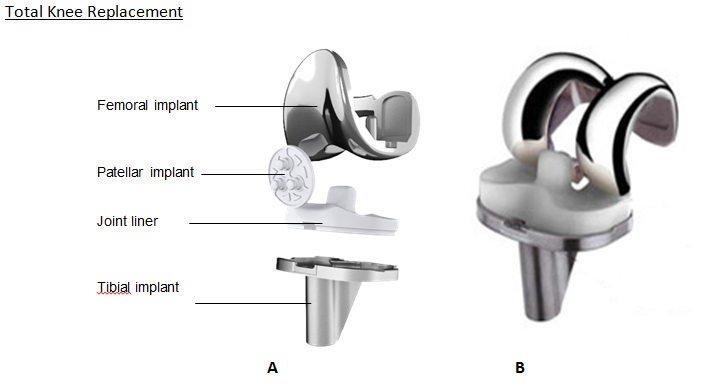
\includegraphics[width=0.7\textwidth]{figures/tka_implant}
\end{center}
\caption{Komponenterne til en total knæalloplastik, består af et femural og tibia implantat ofte bestående af en titaniumlegering. Patella- og tibiaindsatsen er lavet af polyethylen, hvilket er med til at mindske friktionen og efterligne knæledes naturlige bevægelse.\cite{1}} 
\label{fig:tka_implant} 
\end{figure}

Under selve operationen ligger patienten supineret på operationsbordet med knæet i en flekteret position. Et longitudinelt snit lægges over midten af patella. Patella og senerne eleveres og blotter knæleddet, hvilket giver kirurgen adgang til bruskfladerne på femur og tibia. Herefter fjerner kirurgen det ødelagte brusk, ved hjælp af en guideblok der skrues ind i femur og sikrer præcis fjernelse af den ønskede mængde væv. Dette gentages på tibia, hvorved der skabes plads til implantaterne. Midlertidige implantater indsættes for at sikre bevægelsesfriheden er bevaret og testes ved ekstension af knæet for at sikre at den rigtige mænge brusk og knogle materiale er fjernet. Når kirurgen er tilfreds med resultatet bores der guidehuller i henholdsvis femur, tibia og patella til fastemontering af de permanente implantater. Fastmontering sker ved at dække implantatet og monteringsstedet i bencement der limer proteserne fast til den eksisterende knogle struktur. Herefter sikres endnu engang at bevægelsesgraden er bibeholdt, førend indsnittet lukkes og operationen er fuldendt. En TKA operation varer typisk omkring én time, hvorefter patienten kan støtte på benet den følgende dag. Efter operationen følger et rehabiliteringsforløb for at støtte og styrke muskulaturen omkring knæet. \citep{Sanna2013} \citep{tka-technique}

Ifølge sundhedsstyrelsens vurdering er knæalloplastik, effektiv til at mindske smerte, øge funktion og derved bedre livskvalitet. Holdbarheden af knæimplantaterne vurderes ud fra antallet af implantater der er blevet udskiftet efter 10 år, hvor det findes at 90 til 95\%~ af implantaterne ikke er revideret. Dog skal det nævnes at det ikke er muligt at vurdere holdbarheden af den enkelte protese, da flertallet af patienter dør med en velfungerende implantat. \citep{brostrom2012}

\paragraph{Succeskriterier}

Succeskriterier for kirurgisk behandlingen af arterose er ifølge styrringsgruppen for Dansk knæalloplastikregister (DKA) \citep{aarsrapport2016} opdelt i fem kriterier.
%, som alle bygger revisionsraten. Altså patienter som har behov for en yderligere knæ operation.  

% Please add the following required packages to your document preamble:
% \usepackage{graphicx}
% \usepackage[table,xcdraw]{xcolor}
% If you use beamer only pass "xcolor=table" option, i.e. \documentclass[xcolor=table]{beamer}
\begin{table}[H]
\centering
\caption{Tabellen viser succeskriterierne for knæalloplastikoperationer med en standard acceptabel grænse sammenholdt med landsgennemsnittet. Spredning er indikeret i parentes. Tabellen er modificeret fra \citep{aarsrapport2016} }
\label{succeskriterier}
\resizebox{\textwidth}{!}{%
\begin{tabular}{lcc}
\hline
\rowcolor[HTML]{C0C0C0} 
Indikator                                                                                                                                                                                                                                                  & Standard    & \begin{tabular}[c]{@{}c@{}}Landsgennemsnit\\ (Spredning)\end{tabular} \\ \hline
\begin{tabular}[c]{@{}l@{}}\textbf{Genindlæggelse}\\ \\ Andel af alle patienter med primær knæalloplastik på baggrund af primær artrose, \\ der genindlægges uanset diagnose indenfor 30 dage efter udskrivning\end{tabular}                                        & Højest 10\% & 7,3 \% (5,8-9,5)                                                      \\ \\
\begin{tabular}[c]{@{}l@{}}\textbf{Revisionsrate det første postoperative år}\\ \\ Andel af alle patienter med primær knæalloplastik fra et givent operationsår, \\ der er revideret (dvs. implantat fjernes, udskiftes eller tilføjes) indenfor 1 år.\end{tabular} & Højest 3\%  & 1,8 \% (0,8-2,4)                                                      \\ \\
\begin{tabular}[c]{@{}l@{}}\textbf{Revisionsrate de første 2 postoperative år}\\ \\ Andel af alle patienter med primær knæalloplastik fra et givent operationsår, \\ der er revideret (dvs. implantat fjernes eller udskiftes) indenfor 2 år.\end{tabular}          & Højest 5\%  & 3.3\% (1,7-4,8)                                                       \\ \\
\begin{tabular}[c]{@{}l@{}}\textbf{Revisionsrate de første 5 postoperative år}\\ \\ Andel af alle patienter med primær knæalloplastik fra et givent operationsår, \\ der er revideret (dvs. implantat fjernes, udskiftes eller tilføjes) indenfor 5 år.\end{tabular}   & Højest 8\%  & 6,0\% (4,2-6,7)                                                       \\ \\
\begin{tabular}[c]{@{}l@{}}\textbf{Mortalitet indenfor 90 dage}\\ \\ Andel af patienter, der dør indenfor 90 dage efter primær knæalloplastik.\end{tabular}                                                                                                         & Højest 1\%  & 0,4\% (0,0-0,7)                                                      
\end{tabular}%
}
\end{table}

Som det ses af \tabref{succeskriterier} udføres der i hele Danmark knæoperationer som alle signifikant overholder indikationerne for behandlingskvaliteten \citep{aarsrapport2016}. 
På trods af at alle operationer overholder succeskriterier, ses det at patienter postoperativt har smerter og er utilfredse. Antallet af patienter på tværs af studier som er utilfredse er 11 til 25\%, se \tavref{patient_utilfreds} (n=31.114) hvoraf studiet med størst deltagelse (n=27.372) viste at 18\%~ af patienterne var utilfredse. \citep{Bourne2010}

Studiet af \cite{Sakellariou2016} rapporterer postoperative smerter hos patienter, hvor 39\%~(n=272) oplevede moderat til alvorlige smerte\citep{Sakellariou2016}. Et andet studie viste at 19\%~ af patienterne havde svære til uudholdelige smerter efter den første operation. Ved revision var procentdelen af patienter med svære til uudholdelige smerter 47\%. \citep{Petersen2015}

Patienterne burde efter operationen være tilfredse samt smertefri, dette er imidlertid ikke tilfældet. Der er således et problem med resultatet af operationen, på trods af operationen overholder succeskriterierne \citep{aarsrapport2016}. Det må derfor antages problemet ikke ligger ved operationen, men da en del patienter oplever postoperative smerter, er det relevant at undersøge smertes indflydelse på resultatet af operationen. 

%
%(1) http://www.robodoc.com/patient_about_faqs.html
%
%(2) https://www.youtube.com/watch?v=tKji04oFGdU

% (3) http://www.ortopaedi.dk/fileadmin/Guidelines/Referenceprogrammer/Osteotomi_og_TKA.pdf

	%(4) Surgical approaches in total knee arthroplasty.
	
%	(5) tka-technique
%
%(79) Dahl AW, Toksvig-Larsen S, Roos EM. A 2-year prospective study of patient- relevant outcomes in patients operated on for knee osteoarthritis with tibial osteot- omy. BMC Musculoskeletal Disorders 2005;6(1):18. Er lagt på mendlay
%(80) Hoell S, Suttmoeller J, Stoll V, Fuchs S, Gosheger G. The high tibial osteoto- my, open versus closed wedge, a comparison of methods in 108 patients. Arch Or- thop Trauma Surg 2005;125(9):638-643. Er lagt på mendelay
\section{Smerte}

Smerte er blevet defineret som: “en ubehagelig sensorisk og emotionel oplevelse forbundet med egentligt eller potentiel skade af væv eller beskrevet i vendinger tilsvarende en lignende skade.” af den Internationale Association for Studiet af Smerte (Pain) (IASP) [Seminars in arthritis and rheumatism, Classification of Chronic Pain]. 
Selvom smerte normalt er en følelse man forsøger at undgå, er det en nødvendig del af vores overlevelse. Det fortæller kroppen om farer eller skader som der skal reageres på, som for eksempel at sætte hånden på en varm kogeplade. For ikke at blive slemt forbrændt og gøre skade på hånden, registrere nerver i huden en høj temperatur, som hånden skal fjernes fra. Nervesignalet sendes til central nervesystemet (CNS), hvor det først når rygmarven og lidt senere hjernen. Her skelnes der mellem smerte sensation og perception. Smerte sensation er information om smerte, som nerverne i hånden der registrere den skadelige temperatur. Smerte perceptionen sker først når nervesignalet når op til hjernen og denne modtager signalet og opfatter det som smerte. Sensationen af smerte kan i rygsøjlen aktivere en refleks der får musklerne i armen til at trække hånden væk fra varmen, inden hjernen når at registrere og opfatte den egentlige smerte. [Fundamentals of Human Anatomy and Physiologi 9th edition] Denne form for smerte er kategoriseret som øjeblikkelig smerte og defineres som “god” eller “nødvendig” smerte, da det hjælper kroppen med at undgå skader.

\subsection{Smerte typer}
Modsat denne “gode” smerte findes “dårlig” eller “unødvendig” smerte. Denne smerte kaldes også kronisk smerte, da den oftest er længere varende, ved at have været mere eller mindre konstant i mindst tre måneder [Seminars in arthritis and rheumatism]. Personer som lider af kronisk smerte har sjældent en synlig grund til at skulle føle smerte, og smerten er af den grund enten oplevet som smerte i indre organer eller psykogene smerter, som er forestillingen om en smerte. 
Ved organisk smerte skelnes der mellem to typer af smerte: nociceptisk og neuropatisk. Nociceptisksmerte er skade på væv og skyldes aktivering af nociceptorer, specielle nerveceller som er følsomme overfor temperatur ændringer, mekanisk stimuli eller kemiske ændringer i eller omkring celler, ved hjælp af specielle porte og pumper på nervecellerne. Nociceptorer findes i huden på kroppens overflader og i og omkring indre organer, og nociceptisksmerte opdeles i somatisk og viseral sensation. Somatisk smerte sensation og den øjeblikkelige og let placerbare smerte som at sætte hånden på en kogeplade. Viseral smerte sensation er mere besværlig at placere. Smerten er typisk ikke øjeblikkelig, men mere trykkende og langvarig. At have ondt i maven er et eksempel på viseral smerte. Nociceptisksmerte er oftest ikke årsag til kroniske smerter, med mindre smerterne bliver ved. 
Neuropatisk smerte er modsat nociceptisksmerte ikke skade på væv, men på nervesystemet selv, herunder nerver, rygmarv, nerve plexus eller hjernen. Dette kan skyldes direkte skade, sygdom som iskæmi eller sclerose, traume, diabetes, infektioner eller kræft. Smerten kan opleves som konstant og langvarig, hvor er typisk eksempel er fantom smerter, men kan også være lejlighedsvis som ved hyperalgesi, hvor almindelig berøring opfattes som smertefuldt. [Seminars in arthritis and rheumatism, Classification of Chronic Pain] 
Psykogene smerter er en forestillet opfattelse af smerte, og den mest besværlige at præcisere, idet der ikke er og muligvis aldrig har været en fysisk grund til smerten. Hos en person med psykogene smerter er hjernen fuldt overbevidst om, at den oplever fysiske smerter og lider der af. Smerten er udelukkende psykisk hos personen, men er af den grund ikke mindre virkelig, grundet smertes subjektive natur. [Seminars in arthritis and rheumatism]

\subsection{Problemet ved kronisk smerte og operationer}
Der findes således flere forskellige former for smerte, hvor kun nogle få er beskrevet her [Classification of Chronic Pain]. Alle kan de lede til kronisk smerte. Man ved derfor godt hvad der kan give kronisk smerte, hvordan smerten opfattes og hvor i kroppen den kommer fra. Men man ved endnu ikke hvorfor kronisk smerte opstår. Hvorfor føler kroppen fantom smerter fra et legeme som ikke er der? Hvorfor registrere hjernen smerte fra indre organer, når der intet er i vejen med dem? Et større problem opstår når man forsøger at behandle smerterne, med et ønske om at dæmpe eller helt fjerne smerterne, men smerterne fortsætter eller forværres. Sådan ses det i 20\% af tilfælde efter total knæalloplastik (TKA) operationer [Chronic Postoperative Pain After Primary and Revision Total Knee Arthroplasty]. Her oplever 19\% af patienter efter den primære operation, og 47\% af patienter efter revision af operationen oplever svære til uudholdelige smerter. Dette sker på trods af at der i hele Danmark udføres knæoperationer som alle signifikant overholder indikationerne for behandlingskvaliteten [Dansk Knæalloplastikregister, Årsrapport 2016]. De udførte TKA operationer må siges at være nær perfekte, men patienter oplever alligevel fortsatte smerter. 


\section{Klinisk udvælgelse af patienter}\label{kliniskudvaelgelse}
\textit{I dette afsnit undersøges det hvilke retningslinjer og faktorer, der har betydning for en klinikers henvisning af en patient til en TKA-operation. Dette gøres med henblik på en identifikation af eventuelle problematikker ved en udvælgelse af patienter, som hovedsageligt er baseret på en klinikers vurdering.}

Patienter, som tilbydes en TKA-operation, udvælges på baggrund af en klinikerens observationer og erfaringer. Hermed afhænger udvælgelsen af patienter til en TKA-operation af klinikere, hvormed patienter kan opleve varierende anbefalinger og behandlingsmuligheder afhængig af hvilken kliniker, der er ansvarlig for vurderingen. I et forsøg på at standardisere behandlingen af knæartrose for alle patienter i Danmark har Sundhedsstyrelsen udarbejdet en rapport indeholdende nationale kliniske retningslinjer. Disse retningslinjer bygger hovedsageligt på lægelig konsensus. Retningslinjerne vedrørende tilbud om en TKA-operation indeholder blandt andet, at patienter kun tilbydes en TKA-operation hvis non-invasive behandlingsmetoder ikke har en tilstrækkelig virkning. En TKA-operation kan tilbydes patienter som den første behandlingsmulighed, hvis klinikeren vurderer, at patientens artrose er så svær, at ingen non-invasive behandlingsmetoder vil have en tilstrækkelig effekt. Dette kan eksempelvis være, hvis patienten har en kraftig fejlstilling af knæet eller svær instabilitet i leddet. \citep{brostrom2012} \\
Sundhedsstyrelsen har ligeledes opstillet en række indikationer, som kan få klinikeren til at vurderer at en patient ikke er egnet til en TKA-operation. Disse indikationer er eksempelvis, hvis der er infektion i knoglen eller leddet, hvis patienten ingen smerter har i leddet eller hvis patienten har en kort forventet levetid. En anden indikator, som kan få en kliniker til at fravælge at operere patienten, er hvis patienten har urealistiske forventninger til operationen. \citep{brostrom2012} I et studie har \citer{tejada2010} vist, at patienter, hvis forventninger til operationen bliver opfyldt, oplever større tilfredshed efter operationen. Ligeledes er det vist, at klinikerens forventninger til en operation påvirker patientens forventninger \citep{tejada2010}. Dette antyder, at klinikere, ved at forklare patienten hvad de kan forvente af operationen, kan være med til at mindske eller helt fjerne faktoren vedrørende urealistiske forventninger. \\
Ud fra et studie af \citer{skou2016} anses flere af de ovennævnte retningslinjer som nogle af de vigtigste overvejelser, når en kliniker skal bestemme, om en patient er egnet til at modtage en TKA. \citer{skou2016} fandt, at klinikeren anser røntgenresultater, smerte i knæet ved udførelse af hverdagsaktiviteter, funktionelle begrænsninger samt utilfredsstillende virkning af non-invasive behandlingsmetoder som de fire vigtigste faktorer for en patients egnethed til en TKA-operation. Det blev af \citer{skou2016} undersøgt om de faktorer, klinikerne mente var de vigtigste for en patients egnethed for en TKA-operation, blev afspejlet i hvilke patienter klinikerne tilbød en TKA-operation. Her blev det fundet, at radiologiske resultater samt funktionelle begrænsninger var betydningsfulde i forhold til patientens egnethed til en TKA-operation. De to andre faktorer, smerte i knæet samt utilfredsstillende non-invasive behandlinger, var ikke drivende for klinikerens vurdering af patientens egnethed til en TKA-operation. Hermed blev der af \citer{skou2016} fundet en uoverensstemmelse mellem hvilke faktorer klinikerne fandt vigtigst i forhold til vurdering af behovet for en TKA-operation og hvilke faktorer de samme klinikere udvalgte patienter ud fra. Denne uoverensstemmelse viser, hvor kompleks udvælgelsesprocessen for en TKA er samt vanskelighederne ved at bestemme hvilke faktorer, der har størst betydning for en klinikers beslutningsprocess. Ud fra resultaterne fra studiet af \citer{skou2016} antydes det, at klinikerne anvender både bevidste og ubevidste faktorer til bestemmelse af patienters egnethed til en TKA-operation. Flere studier har undersøgt hvilke ubevidste faktorer, der kan påvirke en klinikers beslutningstagning. Eksempelvis antyder resultater fra et studie udarbejdet af \citer{borkhoff2008}, at en patients køn har betydning for, om klinikeren tilbyder patienten en TKA eller ej. I dette studie anvendte \citer{borkhoff2008} to standardiserede patienter med moderat knæartrose, som besøgte 71 klinikere, bestående af 38 alment praktiserende læger og 33 ortopædkiruger. Klinikerne, som deltog i studiet, blev ikke informeret om hvem de to standardiserede patienter var. De to standardiserede patienter var ens på alle andre punkter end køn. \citer{borkhoff2008} fandt, at 55\% af ortopædkirugerne kun tilbød den mandlige patient en TKA-operation, mens ingen af ortopædkirugerne kun tilbød den kvindelige patient en TKA-operation. Sandsynligheden hvormed en patient vil få tilbudt en TKA-operation afhænger af flere parametre. Eksempelvis kan patientens kommunikationsmetode have indflydelse på beslutningen vedrørende det efterfølgende behandlingsforløb. \citep{borkhoff2008}

 % Mulige grunde til den fundne bias i studiet af \cite{borkhoff2008} kan være, at størstedelen af klinikerne der deltog i forsøget var mænd. Ud af de 71 klinikere som deltog i forsøget var 59 af disse mænd. Resultaterne fra studiet viser ingen signifikant forskel i andelen af mandlige klinikere som kun tilbød den mandlige patient en TKA, og andelen af kvindelige klinikere som kun tilbød den mandlige patient en TKA. Det kunne dog undersøges om klinikere har tendens til oftere at henvise patienter af deres eget køn til en TKA end patienter af det modsatte køn. Dette kunne være relevant at undersøge da studier har vist forskelle i mænd og kvinders kommunikationsmetoder, hvormed klinikerens eget køn kan have en betydning for hvordan en patients beskrivelse af sygdommen opfattes og dermed vurderes. \citep{street2002}   
% Bemærk at det med den signifikante forskel handler om mænd vælger mænd etc. Der var en signikant forskel vedr. om det kun er mænd der bliver valgt
I en spørgeskemaundersøgelse, hvor ortopædkiruger blev bedt om at vurdere betydningen af en patients køn i forhold til, om de ville henstille patienten til en TKA-operation eller ej, svarede cirka 93~\% af de adspurgte klinikere, at køn ikke ville have nogen betydning for deres vurdering af patienten \citep{wright1995}. Dette kan antyde, at den forskel \citer{borkhoff2008} fandt i deres forsøg, er følge af en ubevidst bias hos klinikerne. Teorien understøttes også af resultaterne fra et studie udarbejdet af \citer{dy2014}, hvor det blev undersøgt, om en patients race og køn ville have betydning for klinikerens vurdering af patienter.\\
I dette studie blev videoer med patienter med svær knæartrose anvendt. Ligesom i studiet af \citer{borkhoff2008} var patienterne kun forskellige i køn og race. \citer{dy2014} fandt ingen forskel på klinikerens vurdering af de fire standardiserede patienter. Forskellen i resultaterne mellem \citer{borkhoff2008} og \citer{dy2014} kan skyldes forskellen i patienternes grad af artrose. Ved patienter med svær artrose forekom ingen bias, mens der ved patienter med moderat artrose blev fundet bias. Dette antyder, at klinikernes bias kun har betydning for patienter, hvor der ikke er klare indikationer på, at patienten bør opereres.\\
I tilfælde hvor der ikke er klare indikationer på, at patienten vil opnå bedring ved en TKA-operation, vil en teknologi, der kan hjælpe klinikeren med at udføre en vurdering uden bias være fordelagtig. Ved anvendelse af en sådan teknologi vil det være muligt at inddrage andre faktorer i udvælgelsen af patienter til TKA-operation. Dette vil eksempelvis kunne gøres ved at anvende en teknologi, som kan hjælpe klinikere med at vurdere patienters risiko for at udvikle kroniske smerter efter TKA-operationen. Hermed vil det være muligt at mindske fordelingen imellem den tekniske succes og den patientmæssig succes ved en TKA-operation.

Set i forhold til de opstillede succeskriterier for en TKA-operation beskrevet i \secref{tek_succes} er stort set alle TKA-operationer succesfulde, mens omkring 80\% af patienterne, der gennemgår en TKA-operation, ikke oplever kroniske smerter. \citep{Sakellariou2016} \citep{Petersen2015} En succesfuld operation kan dermed defineres forskelligt alt efter hvilken synsvinkel, der arbejdes ud fra. Ud fra en patientmæssig synsvinkel defineres en succesfuld TKA-operation som en operation, hvor patienten er tilfreds med resultatet af denne. Ud fra et teknisk perspektiv er en TKA-operation succesfuld, når denne opfylder kravene opstillet af DKA \citep{aarsrapport2016}. Problematikken opstår ved de TKA-operationer, som kun er succesfulde ud fra et teknisk perspektiv. For at mindske andelen af disse vil det være fordelagtigt at finde en teknologi, som hæver antallet af tilfredse patienter uden at sænke antallet af operationer, som opfylder de tekniske krav. Da kronisk smerte er en af de hyppigste årsager til utilfredshed blandt patienter efter en TKA-operation, vil en reduktion i antallet af patienter med kroniske postoperative smerter sænke antallet af utilfredse patienter. \citep{Bourne2010} 

Udfra disse kriterier vil en teknologi, som gør det muligt at identificere hvilke patienter, der er i risikogruppen for at få kroniske smerter efter en TKA-operation, være fordelagtig. Hermed vil en del af de TKA-operationer, som ikke gavner patienten, kunne undgås. De ovenstående kriterier vil potentielt kunne opfyldes af flere forskellige teknologier. En analyse af disse teknologier vil derfor kunne identificere den mest optimale teknologi til præoperativ undersøgelse af patienter, således patienter med risiko for udvikling af kroniske postoperative smerter kan identificeres.


\textit{I denne sektion vil nuværende teknologier til undersøgelse af neural aktivitet blive beskrevet med særlig fokus på anvendelse i forbindelse med undersøgelse af smerteopfattelse. Det økonomiske aspekt vil ligeledes blive analyseret for de enkelte teknologier. Afslutningsvis vil der blive foretaget en sammenligning med henblik på at identificere fordele og ulemper ved de enkelte teknologier.}
\section{Teknologier til vurdering af smerte} % Anden overskrift...
For at understøtte klinikerens vurdering af de enkelte patienter vedrørende henstilling til TKA, kan det overvejes, hvorvidt det vil være hensigtsmæssigt at tilføje en ekstra undersøgelse til patientens udredningsforløb forud for beslutningen herom. Relevante undersøgelser kan eksempelvis være objektive målinger på neural aktivitet i forskellige situationer, samt vurdering af patienternes individuelle respons på forskellige typer af stimuli. Til undersøgelse af aktivitet i encephalon og nervesystemets funktion generelt findes flere forskellige metoder.
  
\subsection{fMRI}
Functional Magnetic Resonance Imaging(fMRI) er en metode til at undersøge aktiviteten i neuronerne i hjernen.
Generelt er MRI en metode til at synliggøre protoner; dermed er det muligt at afbilde kroppens væv, da dette primært er udgjort af hydrogen-atomer, som indeholder netop én proton.     
Ved en MRI-scanning udsættes objektet, eksempelvis en patient, for et eksternt magnetfelt, hvilket medfører, at der opstår et parallelt magnetfelt i objektet. Dermed er det muligt at detektere de tilstedeværende protoner, da deres retning skaber det parallelle magnetfelt i kroppen.\citep{Wals2009} Udgifterne til fMRI omfatter blandt andet indkøb af MRI-scanner samt anvendelse og vedligehold.\fxnote{Er i tvivl om, om dette er nok, men ellers er man nødt til at anvende sider, der sælger MR-scannere, og det er ikke særligt gode kilder... Alternativt kan der sættes ét priseksempel ind på en konkret scanner?} 
Der findes forskellige teknikker til fMRI, hvoraf de fleste anvender Blood Oxygenation Level-Dependent(BOLD) kontrast. Ved anvendelse af denne kontrast, udnyttes det, at der ved aktivitet i hjernens forskellige områder, vil ske en ændring af mængden af ilt i blodet, hvilket påvirker magnetfeltets styrke. Dermed vil det, ved hjælp af kontrastvæsken, være muligt at følge blodgennemstrømningens styrke i hjernens forskellige områder. \citep{Wals2009} 

\subsubsection{Anvendelse til detektion af smerte}
fMRI har i flere studier været anvendt til at undersøge neural aktivitet i forbindelse med knæsmerter.
I et studie af \citep{Parks2012} er det ved hjælp af fMRI blevet undersøgt, hvorvidt der er forskel på oplevelsen af kroniske smerter hos patienter med artrose og på smerter fremkaldt med tryk. Forsøgsdeltagerne var opdelt i en gruppe patienter med artrose i knæet og en gruppe raske individer. \textbf{xxxx} viste at de to grupper oplevede den kunstigt fremkaldte knæsmerte ens; der forekom stort set ingen variationer imellem de to grupper. Derimod viste der sig at være forskel på de kroniske smerter og de kunstigt fremkaldte smerter hos patienterne med artrose. \citep{Parks2012} 
I et andet studie af \citep{Hiramatsu2014} er det undersøgt, hvilke forskelle der forekom i cerebral respons hos en gruppe raske forsøgspersoner og en gruppe forsøgspersoner med kroniske knæsmerter forårsaget af artrose. Begge grupper blev udsat for akut smerte gennem invasive elektroder imens der blev foretaget en fMRI scanning. Studiet viste, at der hos gruppen af patienter med kroniske knæsmerter forekom en højere aktivitet i det dorsolaterale præfrontale cortex end hos gruppen af raske forsøgspersoner. \citep{Hiramatsu2014} 
fMRI kan således påvise forskelle på hvordan smerte opleves af forskellige grupper af mennesker. Figur \ref{fig:fMRI_result} illustrerer forskellen i neural aktivitet mellem patienterne og den raske forsøgsgruppe.
\begin{figure}[H] 
	\begin{center}
		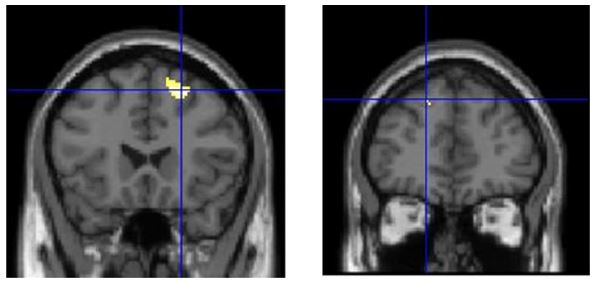
\includegraphics[width=0.7\textwidth]{figures/bProblemanalyse/fMRI_dorsolateral}
	\end{center}
	\caption{Figuren illustrerer forskellen imellem henholdsvis patientgruppen og den raske forsøgsgruppe. Det fremgår, at aktiviteten i det dorsolaterale cortex er signifikant højere hos patienterne end hos de raske individer. \citep{Hiramatsu2014}} 
	\label{fig:fMRI_result} 
\end{figure} 

\subsection{Quantitative sensory testing}
Quantitative sensory testing(QST) er en metode til undersøgelse af det sensoriske nervesystems funktion. Metoden kan anvendes til undersøgelse af forskellige egenskaber, herunder smertegrænser. Ved en QST-undersøgelse eksponeres patienten for forskellig sensorisk sensation, herunder tests, der involverer varme og kulde, vibration og tryk. Dermed er det muligt at identificere grænserne for henholdsvis perception og smerte. \citep{Yarnitsky2006} QST kræver - i modsætning til fMRI - ikke scanning eller anden billeddiagnostisk undersøgelse. 
Der findes forskellige protokoller til QST-undersøgelse, der alle indeholder tests indenfor de forskellige områder, der ønskes undersøgt ved en QST. Et eksempel er en QST-protokol udviklet af German Network on Neuropathic Pain til undersøgelse af neuropatisk smerte. Ved brug af denne model anvendes syv forskellige tests til at vurdere 13 parametre, herunder seks temperaturtests til detektion af grænser for perception og smerte samt syv mekaniske tests til detektion af tilsvarende grænser, her med henholdsvis spidste og stumpe genstande. I forbindelse med udarbejdelse af modellen er der desuden lavet tests for at opstille referenceværdier, der tager højde for både køn og alder. citep{8}  

\subsubsection{Anvendelse til detektion af smerte}
QST bliver i forskningsregi anvendt til undersøgelse af patienter der får udført TKA. I et studie af \citep{Martinez2007} er en anden QST-protokol anvendt til at undersøge 20 patienter med artrose i knæet før og efter en TKA. Formålet hermed var at identificere faktorer, der har indvirkning på udviklingen af postoperative smerter efter operationen. QST-undersøgelserne blev udført henholdsvis før operationen og efterfølgende en og fire dage samt en og fire måneder efter operationen. Parametrene der blev undersøgt i QST-undersøgelsen var tærskelværdier for temperatur, mekanisk smerte og hvordan de enkelte patienter responderede på en eksponering for temperaturer over tærskelværdierne. Studiet fandt, at der forekommer en sammenhæng mellem periodiske smerter efter operationen og de patienter, der oplever hyperalgesi under eksponering for varme. \citep{Martinez2007} Der skal imidlertid tages højde for, at der er flere fejlkilder forbundet med QST-undersøgelser, da nøjagtigheden i høj grad afhænger af både patientens og undersøgerens præcision under udførelsen af de enkelte tests. Det må således forventes, at der kan forekomme variationer mellem enkelte QST-undersøgelser udført på den samme patient. \citep{Yarnitsky2006}

\subsection{Elektrofysiologiske undersøgelsesmetoder}
De elektrofysiologiske undersøgelsesmetoder dækker over tests, der kontrollerer elektrisk aktivitet i kroppens celler. I hviletilstand har et neuron en fast spænding over sin membran. Når dette membranpotentiale ændres som følge af ændringer i koncentrationen af natrium- og kaliumioner inden- og udenfor cellen, genereres et aktionspotentiale, som vandrer langs cellens akson og videre til de følgende neuroner. Dette kan detekteres ved anvendelse af invasive eller noninvasive elektroder. Til monitorering af neuronernes funktionalitet i encephalon anvendes elektroencephalografi (EEG) mens der til monitorering af neuronernes funktionalitet i resten af kroppen anvendes elektroneurografi (ENG). For at en elektrofysiologisk undersøgelse kan anvendes til at stille en diagnose, skal resultaterne herfra understøttes af andre kliniske undersøgelser, herunder prøver og lægesamtaler. \citep{Robinson2008} 

\subsubsection{Anvendelse til detektion af smerte}
I et studie af \citep{Brown2013}, er EEG blevet anvendt til at undersøge, hvordan to patientgrupper med forskellige sygdomme opfatter smerte. I studiet indgik en gruppe af patienter med artrose og en gruppe patienter med sygdommen fibromyalgi, der forårsager muskel- og ledsmerter \citep{Brown2013}\citep{9}. Hos de to patientgrupper blev det undersøgt, hvordan encephalon genererer signal for henholdsvis en forventning om og en decideret udløst smerte. Disse data sammenlignes med en kontrolgruppe bestående af raske, smertefri personer. Der blev foretaget to målinger for at undersøge aktiviteten under forventning om smerte samt en måling under påført smerte. For hver forsøgsperson blev det efter målingerne undersøgt, fra hvilken elektrode, der dektekterede den højeste amplitude, hvormed denne og de otte nærmeste elektroder blev udvalgt til yderligere analyse og udregning af gennemsnitlig amplitude. De gennemsnitlige målinger for de tre forsøgsgrupper er illustreret i figur \ref{fig:EEG_gns}.
\begin{figure}[H] 
	\begin{center}
		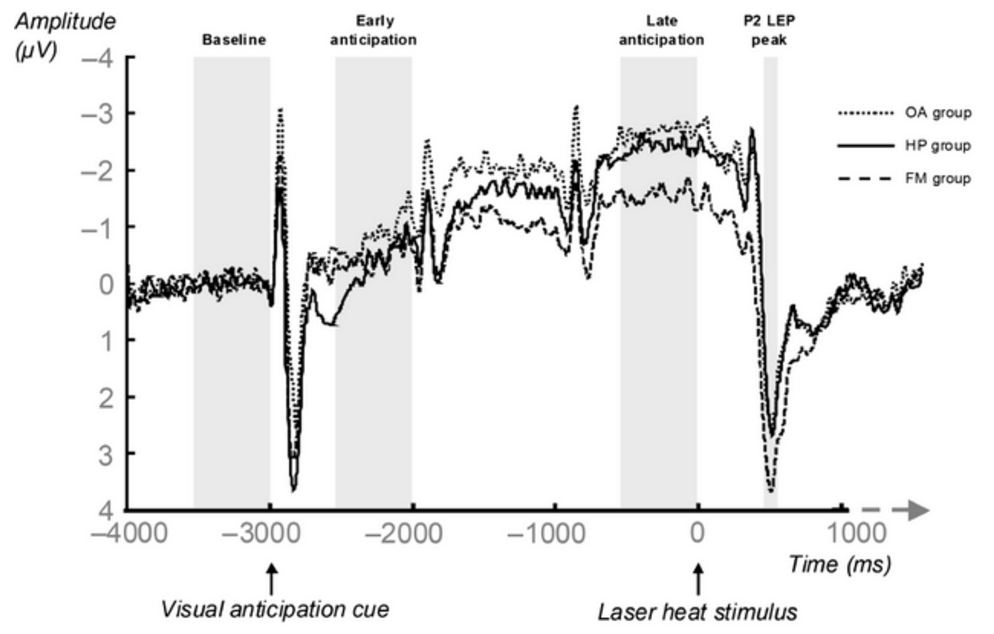
\includegraphics[width=0.7\textwidth]{figures/bProblemanalyse/EEG_ERP}
	\end{center}
	\caption{Figuren illustrerer de gennemsnitlige målinger for de tre forsøgsgrupper. Tidspunkter for måling af baseline, tidlig forventning, sen forventning og oplevelse af smerte er angivet på figuren. \citep{Brown2013}} 
	\label{fig:EEG_gns} 
\end{figure} 
Ud fra resultaterne var det muligt at undersøge i hvilke områder, der forekom særlig aktivitet ved hjælp af blandt andet billeddannende programmer. Resultaterne for studiet antyder, at de to patientgrupper responderer ens på forventningen om smerte, på trods af, at fibromyalgipatienternes respons var kraftigere. Disse resultater indikerer, at denne tendens kan være generelt gældende for patienter med kroniske smerter. \citep{Brown2013} Udgifterne til EEG-undersøgelse omfatter indkøb af udstyr samt løn til medarbejderne, der er med til at udføre undersøgelsen\citep{Green1985}.  
 % 1 = fMRI techniques and protocols
 % 2 = The dorsolateral prefrontal network is involved in pain perception in knee osteoarthritis patients
 % 3 = Brain activity for chronic knee osteoarthritis: dissociating evoked pain from spontaneous pain
 % 4 = Quantitative sensory testing
 % 5 = The evolution of primary hyperalgesia in orthopedic surgery: Quantitative sensory testing and clinical evaluation before and after total knee arthroplasty
 % 6 = Clinical electrophysiology
 % 7 = When the brain expects pain: common neural responses to pain anticipation are related to clinical pain and distress in fibromyalgia and osteoarthritis 
 %10 = Benefits, Shortcomings, and Costs of EEG Monitoring
\chapter{Problemafgrænsning}\vspace{-.75cm}
\newpage \section{Problemafgrænsning}
Selvom operationerne bliver udført ‘perfekt’ så er 11 til 25\% af patienterne stadig utilfredse. Det tyder på at disse patienter er utilfredse pga. deres manglende resultater efter operationen, relateret til smerte og funktionsnedsættelse. Klinikerne er ansvarlig for belsutningstagen hvorvidt en patient er egnet til at modtage en TKA-operation. Klinikerne formår succesfuldt at udvælge 75 til 81\% af patienterne, på baggrund af deres erfaring, radiologiske fund, symptom vurdering, samt patientens egne udtalelser. Den resterende patientgruppe er utilfredse med resultatet, hvilket indikerer at udvælgelsesmetoden ikke er god nok, og at eventuelle bias kan have medvirket til dette resultat. Det kunne derfor, for klinikeren og patienten være fordelagtigt hvis den benyttede metode blev optimeret. Optimeringen kunne indebære afbenyttelse af en teknologisk metodik. Den teknologiske tilgang skulle medføre nogle faktiske resultater som skal supplere og bidrage til klinikerens beslutningstagen. Hvis en teknologisk metode skal kunne implementeres kræves det at denne muliggør identificering af patientgruppen, hvis risiko for kroniske komplikationer postoperativt, er størst. Den teknologiske tilgang bør ydermere være minimalt invasiv, omkostningseffektiv og let organisatorisk implementerbar. Disse kriterier opfyldes på bedste vis af QST, blandt de analyserede smertediagnosticeringsmetoder, hvormed det antydes at QST vil være den teknologiske tilgang som bedst vil kunne supplere klinikerens beslutningstagen. 

\subsection{Problemformulering}
\begin{center}
	\textit{Hvilke konsekvenser er der forbundet med en implementering af QST som supplement til klinikerens vurdering af patienten til indstilling til TKA, på de ortopædkirurgiske afdelinger i Region Nordjylland?}
\end{center}

%%%%%%%%%%%%%%%%%%METODE%%%%%%%%%%%%%%%%%%%%%%%%%%%%
\chapter{Metode}\vspace{-.75cm}
\textit{kursiv afsnit}

\section{Projektets metode}
I dette projekt anvendes HTA-core modellen, hvilket afspejles i projektets metode. Målet med anvendelse af HTA-core modellen er at analysere og diskutere de essentielle problemstillinger ved QST, samt at præsentere resultaterne fundet ved analysen og diskussionen \citep{HTAcore}. Ydermere bidrager benyttelsen af HTA-core modellen til en systematisk og bred vurdering af QST. Dette giver et evidensbaseret grundlag til beslutningstagning i forhold til eventuel implementation af QST. \citep{metodehaandbogen} \citep{HTAcore} HTA-core modellen anvendes til besvarelse af problemformuleringen, da denne lægger op til en analyse af væsentlige faktorer ved QST, set ud fra et sundhedsvidenskabeligt perspektiv. Ved anvendelse af HTA-core inddeles analysen af teknologien i ni forskellige områder \citep{HTAcore}:

\begin{enumerate}
\item Sundhedsmæssigt problem og nuværende brug af teknologien (CUR)
\item Beskrivelse og tekniske karakteristika for teknologien (TEC)
\item Klinisk effekt (EFF)
\item Sikkerhed (SAF)
\item Organisatoriske aspekter (ORG)
\item Patient- og sociale aspekter (SOC)
\item Etisk analyse (ETH)
\item Juridiske aspekter (LEG)
\item Omkostninger og økonomisk evaluering (ECO)
\end{enumerate}

Benyttelsen af HTA-core modellen illustreres på \figref{fig:VORESMODEL}. I dette projekt er områderne opsat som det fremgår af rækkefølgen ovenover, men som det ses ud fra \figref{fig:metode}, er der et sammenspil mellem områderne. 

\begin{figure}[H] 
	\begin{center}
		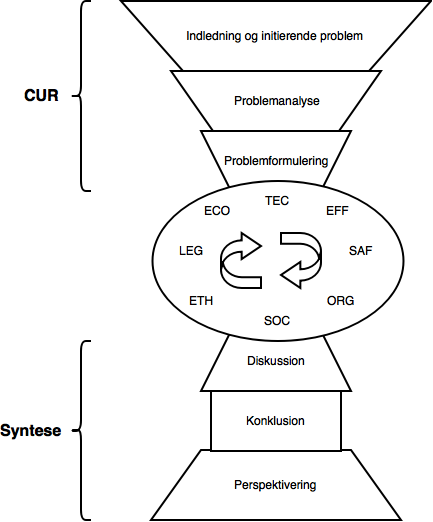
\includegraphics[width=0.5\textwidth]{figures/cMetode/metode}
	\end{center}
	\caption{VORES-model, der anvendes i projektet. Det ses, hvordan...} 
	\label{fig:metode} 
\end{figure}

Som det ses ud fra \figref{fig:metode} 
\textbf{Argument for overgangen mellem billedet her og næste afsnit om vurderingselementer}

Vurderingselementer er en betegnelse for det samlede produkt for analysen af et af de ni områder. Hvert domæne bliver inddelt i emner der hver skal klarlægge et bestemt problem indenfor området. Hvert emne specificeres yderligere ved konkrete HTA-spørgsmål, som skal besvares for at kunne besvare problemformuleringen. Når et eller flere HTA-spørgsmål under et emne er besvaret, kan besvarelsen af emnet samles med svar fra andre emner i domænet, i en delkonklusion. Delkonklusionen er besvarelsen af et domæne, og svaret indgår som et vurderingselement til den endelige besvarelse af problemformuleringen. \citep{HTAcore} \Figref{fig:vurderingselement} viser den beskrevne opbygning af vurderingselementet. 

\begin{figure}[H] 
\begin{center}
\includegraphics[width=0.5\textwidth]{figures/cMetode/vurderingselement}
\end{center}
\caption{Opbygningen af et vurderingselement. Figuren viser, hvordan vurderingselementet samlet er udgjort af de tre elementer; område, emne og problematik.}
\label{fig:vurderingselement} 
\end{figure}

I dette projekt opstilles analyseområderne med inspiration fra retningslinjerne i håndbogen for HTA-core modellen. Disse retningslinjer omfatter blandt andet hvilke emner, der bør afdækkes indenfor de enkelte domæner samt generelle forslag til spørgsmål. Det fremgår desuden, hvilke andre vurderingselementer, domænet relaterer til. Herudover angives det, hvilken metode og hvilken type litteratur, der kan være medvirkende til at besvare et givent domæne. \citep{HTAcore} \\
Afslutningsvis vil de enkelte vurderingselementer og problemformuleringen, sammenfattes i en syntese indeholdende en diskussion af resultater og en konklusion på problemformuleringen. 

\subsection{Argumentation for valg af domæner}
Før besvarelse af hvert domæne, argumenteres der for det enkelte domænes relevans for besvarelsen af problemformuleringen. Dette skal sikre at kun de vurderingselementer der bidrager til besvarelse af problemformuleringen besvares i projektet. 

Det første domæne, CUR, lægger op til analyse af et sundhedsmæssigt problem og mulige løsninger på problemet. Hermed er domænet relevant for dette projekt, idet det er gennem CUR-domænet det problem som resten af domænerne forsøger at besvare findes. CUR-domænet besvares ved benyttelsen af en AAU-inspireret tilgang. Først indledes projektet med et initierende problem, der lægger op til en bred, alsidig undersøgelse af relevante aspekter for projektet, hvilke undersøges i problemanalysen for at finde et konkret problem, som ønskes besvaret. Igennem analysen bliver det initierende problem undersøgt og afslutningsvis afgrænset, hvormed der kan opstilles en problemformulering. Problemformuleringen definerer det konkrete problem, og besvares igennem de resterende domæner i HTA-core modellen. De første to kapitler (\chapref{introduktion} og \chapref{problemanalyse}), udgør dermed i dette projekt CUR analysen. De resterende områders metode vil blive beskrevet i deres respektive analyser. 

I domænet TEC undersøges den valgte teknologi, både i forhold til oprindelige formål og hvordan teknologien kan anvendes i forhold til det opstillede problem. Idet QST er en gammel metode, som indeholder et stort spænd af protokoller er det relevant at inddrage TEC domænet, for at få et indgående kendskab til både den generelle QST og de QST-parametre som anvendes til undersøgelse af knæartrosepatienter. Ligeledes er et kendskab til QST, dennes krav til patienter og brugere samt mulighederne for samspillet mellem QST og klinikeren nødvendige før det er muligt at analysere flere af de andre domæner. 

Domænet EFF har til formål at analysere en teknologi ud fra dens effektivitet og virkningsgrad. Idet QST-undersøgelser af knæartrosepatienter er et relativt nyt tiltag, vil det være relevant at undersøge hvor effektive disse undersøgelser er i forhold til sensitivitet og specificitet. Dette domæne er ligeledes en relevant del af projektet idet overvejelser fra området kan inddrages i eksempelvis ECO-området.   


Ved SAF-området undersøges sikkerhedsrisici ved en teknologi. Ved QST-undersøgelser tilpasset kroniske postoperative smerter tilføres en patient smerte for at vurdere patientens reaktion ud fra forskellige parametre. Hermed kan der være sikkerhedsmæssige risici for patienten, hvilket kan føre til eventuelle skader. Det er dermed relevant at undersøge om de undersøgelsesmetoder der anvendes i QST kan skade patienten samt i hvilket omfang dette kan ske. Dette gør det muligt at vurdere hvorvidt de sikkerhedsmæssige risici ved QST-undersøgelserne overgår den diagnostiske relevans for undersøgelserne. 

\textbf{ORG}

\textbf{SOC}

Ved ETH-domænet undersøges de etiske aspekter ved en teknologi. Da QST skal anvendes som vurderingsgrundlag forud for en operation vil det have etiske konsekvenser, hvis QST ikke kan identificere alle patienter med forhøjet risiko for udvikling af kroniske postoperative smerter. Disse overvejelser vil både gælde for falsk positive og falsk negative resultater. \textbf{Tilføj hvad end er besluttes ift nye spørgsmål}       

\textbf{LEG}

I ECO-domænet undersøges problemet ud fra et økonomisk synspunkt. Da det for QST-undersøgelserne er nødvendigt at anvende teknologisk udstyr, er der omkostninger forbundet med implementering af disse. Ligeledes vil der blandt andet være omkostninger ved oplæring af personale. Disse økonomiske omkostninger sættes op imod gevinster ved implementeringen af QST. Disse gevinster kan være både monetære eller tage anden form. Det er relevant at undersøge implementeringen og brugen af QST ud fra et økonomisk perspektiv, idet dette er en betydelig del af et politisk vurderingsgrundlag. 

\subsection{Litteratursøgning} \label{sec_lit}
Litteratursøgning og -vurdering i projektet tager udgangspunkt i retningslinjerne opstillet i Metodehåndbogen for Medicinsk Teknologivurdering udarbejdet af Sundhedsstyrelsen \citep{metodehaandbogen}. Da projektet udarbejdes på baggrund af videnskabelig litteratur, er det væsentligt, at litteraturen findes og vurderes ved en organiseret fremgangsmåde, således at problemformuleringen besvares på et veldokumenteret grundlag. Litteratursøgningen vil derfor være den samme for alle områder af rapporten. For hvert domænes metode vil litteratursøgning kun beskrives i så fald søgningen for det specifikke område afviger fra den generelle litteratursøgningsmetode som beskrevet her. \\
Generelt for litteratursøgning vil der blive søgt på sundhedsvidenskabelige databaser som: PubMed, MEDLINE, EMBASE og Cochrane Library. Aalborg Universitetsbiblioteks søgemaskine Primo vil ligeledes tages i brug og anvendes som generel søgeværktøj, da denne dækker mange databaser. For ligeledes at sikre ensartethed gennem rapporten vil udvælgelsen og vurderingen af litteratur forløbe efter samme søgestrategi for alle områder. 

Litteratur er søgt således, at antal hits per søgning, befinder sig ~100. Dette betyder at alle overskrifter for den pågældende søgning er blevet gennemgået for relevans. Ved de udvalgte artikler, er abstract efterfølgende blevet gennemlæst for at sortere materialet. De artikler som er blevet fundet relevante til besvarelse af HTA-spørgsmålet, er blevet kritisk gennemgået. Ved enkelte artikler er snowballing blevet benyttet. Her gennemlæses fundne studiers referenceliste og relevante studier herfra anvendes til besvarelse af HTA-spørgsmålet.

Søgeprotokollen har ligeledes til formål at gøre det muligt for interessenter at forstå, hvordan litteratursøgningen er forløbet. \citep{metodehaandbogen} Til at udarbejde søgeprotokollen i dette projekt, er der opstillet en skabelon, der systematiserer litteratursøgningen. Et uddrag af skabelonen ses i \figref{fig:soegeprotokol}.

\begin{figure}[H]
\begin{center}

\includegraphics[width=0.5\textwidth]{figures/cMetode/soegeprotokol}
\end{center}
\caption{Skabelon for projektets søgeprotokol. Det fremgår af skabelonen, at der for hver søgning skal opstilles ét HTA-spørgsmål samt inklusions- og eksklusionskriterier. Det skal ligeledes dokumenteres, hvilke databaser, der er anvendt til søgningen. For hver database skal de specifikt anvendte søgeord opstilles, og antallet hits skal efterfølgende fremgå.}
\label{fig:soegeprotokol} 
\end{figure}

HTA-spørgsmålet i søgeprotokollen har til formål at bidrage til besvarelsen af problemformuleringen indenfor de otte domæner. Spørgsmålene skal være helt afgrænsede og entydige, således at det er muligt at finde konkret litteratur, og besvare dem præcist. \citep{metodehaandbogen}  
For at afgrænse og sikre relevansen af søgeresultaterne, opstilles inklusions- og eksklusionskriterier for søgningerne. Søgningerne kan eksempelvis afgrænses til kun at indeholde bestemte typer studier, en eller få specifikke sygdomme, en afgrænset aldersgruppe med mere. \citep{metodehaandbogen} \\
Dokumentationen af valgte databaser samt tilhørende specifikke søgeord er en væsentlig del af søgeprotokollen, da databaserne har forskellige typer syntaks til litteratursøgning, hvormed det er vigtigt, at søgningen i en given database er foretaget med anvendelse af søgetermerne specifikke for den valgte database. \citep{metodehaandbogen}
Efter litteratursøgningen vurderes den fundne litteratur med henblik på at udvælge de kilder, der bedst kan besvare de fokuserede spørgsmål og dermed den overordnede problemstilling for projektet. Det er således essentielt at kontrollere, om det, der undersøges i udvalgt litteratur, har relevans for de fokuserede spørgsmål eksempelvis ved gennemlæsning af abstract, metode samt resultater. Ligeledes vurderes studiers evidensniveau, for at sikre kvaliteten af besvarelserne. \citep{metodehaandbogen} 
Litteraturen i dette projekt inddeles ud fra evidenshierakiet i \citer{metodehaandbogen}. Evidenshierakiet omfatter følgende syv punkter, hvor kilder med det højeste evidensniveau er placeret øverst i listen:

\begin{enumerate}
\item Metaanalyser og systematiske undersøgelser 
\item Randomiserede kontrollerede undersøgelser (RCT’s)
\item Ikke-randomiserede kontrollerede undersøgelser
\item Kohorte undersøgelser
\item Case-kontrol undersøgelser
\item Deskriptive undersøgelser, mindre serier
\item Konsensusrapporter, ikke-systematiske oversigtsartikler, ledere, ekspertudtalelser
\end{enumerate}

Metaanalyser og systematiske undersøgelser er sekundær litteratur og har det højeste evidensniveau. Denne type litteratur er statiske sammenfatninger af primær litteratur med samme afgrænsede problemstilling. \citep{denstoredanske2009} \\
Randomiserede kontrollerede undersøgelser (RCT) er primær litteratur, hvor der foretages en sammenligning af to forsøgsgrupper. Den ene gruppe udsættes for en påvirkning, mens den anden gruppe fungerer som kontrolgruppe. Udvælgelsen af forsøgspersoner foregår tilfældigt. \citep{denstoredanske2009a} \\
Ikke-randomiserede kontrollerede undersøgelser er ligesom RCT’s primær litteratur, hvor to forsøgsgrupper sammenlignes. Ved disse undersøgelser sker udvælgelsen af forsøgspersoner ikke tilfældigt, hvormed evidensniveauet falder da der ikke på samme måde som ved RCT tages højde for bias i forsøgsgrupperne. \citep{denstoredanske2009a} \\
Ved kohorte undersøgelser følges flere forsøgsgrupper over en periode for at undersøge, hvorvidt bestemte eksponeringer har indflydelse på udviklingen af helbredsfænomener, herunder sygdom og død. \citep{metodehaandbogen} \\
I case-kontrol undersøgelser, forsøges det at undersøge forskellige faktorers indflydelse på udvikling af bestemte sygdomme. Dette gøres ved en sammenligning mellem en forsøgsgruppe med den pågældende sygdom og en forsøgsgruppe bestående af raske personer. I modsætning til eksempelvis kohortestudiet følges forsøgsgrupperne ikke over tid, hvormed der ikke kan udføres en opfølgende undersøgelse. Det er således ikke muligt at estimere betydningen af  risikofaktorerne. \citep{denstoredanske2012} \\
Deskriptive studier er studier hvor der foretages analyser til beskrivelse af et fænomen. I modsætning til de andre typer studier påvirkes forsøgsgrupperne ikke. I stedet undersøges nuværende tendenser, eksempelvis med henblik på senere udførelse af et forsøg. \citep{} \\
Fælles for gruppen af konsensusrapporter, ikke-systematiske oversigtsartikler samt ledere og ekspertudtalelser er, at materialet oftest er udtryk for subjektive holdninger, der ikke er underbygget af tilstrækkelige mængder supplerende litteratur, der undersøger området. \citep{metodehaandbogen}  \label{metode}

%%%%%%%%%% HTA - analyse %%%%%%%%%%%%%%%%%%%%%%%%
\chapter{Beskrivelse og tekniske karakteristika for teknologien (TEC)}\vspace{-.75cm} \label{TEC_chap}
\section{Formål}
I teknologidomænet analyseres QST som et teknologisk supplement til klinikerens vurdering af en patients henvisning til en TKA-operation.  For at muliggøre dette kræves et kendskab til både klinikerens vurdering, og QST. Gennem problemanalysen er klinikernes vurdering undersøgt, mens teknologidomænet danner grundlag for kendskab til QST.\\
For at opnå et kendskab til QST forventes en forståelse for teknologiens egenskaber, virkemåde samt begrænsninger. Heraf undersøges det oprindelige formål med QST, med henblik på at bestemme, hvordan denne er tilpasset og brugt i sammenhæng med TKA-operationer. Dette bidrager til at vurderingsgrundlaget for hvorvidt QST kan fungere i samspil med klinikeren. Ydermere er det nødvendigt at vide hvad QST kan, hvordan dette er muligt, samt hvordan teknologien begrænses. Hermed er det muligt at vurdere hvordan og i hvilket omfang QST vil kunne fungere som supplement til klinikeren.\\
Da der er blevet tilegnet et kendskab til QST, er der grundlag for at undersøge og sammenligne QST med klinikerens vurdering. En sammenligning af QST med klinikerens metode er nødvendig for at kunne vurdere hvorvidt QST har evnen til at fungere som supplement hertil. 
\section{HTA spørgsmål}
\textit{Teknologiens egenskaber:}
\begin{itemize}
	\item Hvad er teknologiens oprindelige fokusområde og hvordan er den tilpasset knæartrose på nuværende tidspunkt? %B0003, A0022
	\item Hvordan virker teknologien?  %B0001
\end{itemize}

\textit{Teknologiens begrænsninger:}
\begin{itemize}
	\item Hvilke eksterne faktorer kan påvirke QST-resultaterne?
\end{itemize}

\textit{Sammenligning med nuværende metoder:}
\begin{itemize}
	\item Hvordan adskiller QST-teknologien og den nuværende medicinske teknologi sig fra hinanden? %B0001, B0002
\end{itemize}

\section{Metode \citep{HTAcore}}
Vidensindsamlingen til besvarelse af det teknologiske område vil foregå ved at søge efter materiale igennem HTA/MTV agenturer, i relevante sundhedssystemer og sundhedsudbydere. Databasen der anvendes afhænger af hvilket spørgsmål det søges at besvare. Til indsamling af viden omhandlende de tekniske fakta vedrørende teknologien vil der blive benyttet relevante datablade fra producenter, beskrivende reviews samt ekspertudtalelser fra personel som benytter teknologien, hvis nødvendig. Til besvarelse af hvordan teknologien er udviklet, samt benyttet vil der hovedsageligt blive benyttet reviews fra anerkendte databaser (PubMed, Medline, the Cochrane Library) samt bøger.  \\
Til besvarelse af TEC-analysen bestræbes det at undgå grå litteratur, men i tilfælde, hvor der foreligger begrænsede mængder videnskabelig litteratur, kan der supplementeres med non-peer reviewed-, ikke-publiceret materiale, fortroligt kommercielt materiale samt generelle internetsøgninger.

\section{Fokusområde for QST og tilpasningen til knæartrose}
I perioden omkring det 19-århundrede blev der udviklet flere medicinske værktøjer til kvantitativ vurdering af sensation. Vurderingselementerne omhandlede klassificering af tærskelværdier, tolerancer og stimuli-respons forhold. Nødvendigheden af at kunne kvantificere en tilstand er en essentiel faktor for et hvert videnskabeligt resultat. Validiteten af et videnskabeligt resultat bør altså delvist dannes på grundlag af en kvantificering af relevante parametre. \citep{Yarnitsky2006} Videnskabsmændene i det sene 19-århundrede beskæftigede i større grad tilstande som ikke forvoldte smerter, og heraf blev de mest populære fund relateret til de termiske sanser samt vibrationssensation. \citep{Yarnitsky1997} QST muliggør dog at undersøge tilstande ved benyttelsen af andre stimuli. QST omfatter termisk, mekanisk og elektrisk, iskemisk og kemisk. De forskellige stimuli bidrager til at kunne undersøge forskellige parametre. Parametrenes reaktion på de forskellige stimuli kan klassificeres som værende af forringet effekt eller forøget effekt.

Til klassificering af tærskelværdier samt tolerancer bliver der generelt benyttet to basisgrupperinger, med- og uden reaktionstid. Der er blevet udviklet flere metoder til begge af disse basisgrupperinger. Grundlæggende for metoderne omhandlende reaktionstid er transmissionstiden fra et påført stimuli til reaktion. Ved metoder uden benyttelse af reaktionstid indebærer det oftest 'ja/nej' reaktioner til intensitetsforudbestemte stimuli, hvorefter intensiteten ændres.\fxnote{Method of levels, Method of limits} \citep{Yarnitsky1997} 

QST betegnes som en subjektiv vurderingsmetode, da det omfatter en subjektiv respons, som befindes indenfor et psykofysisk parameter, til et kontrolleret stimuli. Den subjektive respons er på baggrund af patienten deltager under frivillig kontrol. \citep{Mucke2016} I og med vurderingsmetoden er subjektiv, kan resultatet påvirkes af distraktioner, kedsommelighed, mental træthed og forvirring. Ydermere kan en subjektiv respons ydermere bidrage til at patienten bevidst fejlrapporterer på baggrund af en interessekonflikt i resultatet. \citep{Yarnitsky2006} 

Betydningen af at QST er en subjektiv vurderingsmetode, bør behandlingen omfatte kvalitetskontrol. Det nævnes af \citer{Yarnitsky2006} at resultater opnået med 'Method of Limits' imellem sessioner kan variere op mod 150\%. Mens ved benyttelsen af en anden algoritme, opstod en individuel variation på 5\%. For at sammenligne resultater imellem sessioner er korrelationsteknikker blevet kritiseret. Kritikken opstår på baggrund af at korrelationsteknikken måler styrken af forholdet, og ikke hvor ens disse er. En tilgang som blev fremstillet mere pålidelig er at udregne en repeterbarhedsfaktor (r), da med et konfidensinterval på 95~\%, vil to resultater fra samme patient, vil afvige med mindre end r-faktoreren. Dog er skal det tages højde for at det kan være problematisk at udføre statistiske beregninger mellem grupper. Dette er tilfældet da resultaterne stammer fra subjektive vurderinger. \citep{Zaslansky1998} I relation afbenyttelse af normativ data vedrørende tærskelværdier og toleranceværdier skal den eksakte metodik benyttelse. Hvis ikke der tages højde for den eksakte metodik vil resultaterne sandsynligvis ikke være repræsentative og heraf afvige fra normalen der tages udgangspunkt i. \citep{Yarnitsky1997}

\subsection*{Klinisk anvendelse af QST}
QST bliver benyttet i flere kliniske sammenhænge. I mange tilfælde bliver QST benyttet som et diagnostisk værktøj, men kan også bruges til at vurdere omfanget af en sensorisk lidelse. Generelt er bliver QST benyttet til at kunne klassificere sygdomme relateret til CNS, heraf flere omhandlende sensationstab. Dette er også tilfældet ved benyttelsen relateret til diabetes. 50\% af diabetikere har perifer neuropati, og ved benyttelse af en termisk metode af QST, kan man tidligt i patologien identificere dette. Neuropati er ligeledes fundet ved mange med nyresvigt, hvilket kan klassificeres med igennem undersøgelse af vibrationssensation og termisksensation. \citep{Yarnitsky1997} \citep{Yarnitsky2006} \\
QST bliver også benyttet til at klassificere smerter, men til dette er der relateret en bred problemstilling. Problematikken opstår i og med det psykofysike og psykologiske som QST er bestående af, samt forskellig smerteopfattelse og smertereaktion. \citep{Yarnitsky1997} Det er anerkendt at mennesker har forskellige smertemønstre i relation til smerte stimuli. Det kan varierer fra at være yderst følsom til at være upåvirket. Forståelsen af disse smertemønstre, kan med den korrekte QST tilgang, bidrage til at kunne forudsige responsen af en given interaktion. \citep{Yarnitsky2006} Ydermere kan QST i smerteregi, klinisk blive benyttet til at lave kvalitative sammenligninger mellem forskellige grupperinger \citep{Arendt-Nielsen2009}. \\
Dog menes det generelt, at QST-resultater ikke, som det eneste resultat, kan benyttes til at stille en diagnose. Dette er på baggrund af tidligere nævnte årsager relateret til det subjektive aspekt i metoden. \citep{Yarnitsky2006}

\subsection*{Tilpasning af QST til knæartrose}




































%  Yarnitsky-1997-Muscle_&_Nerve.pdf [1]
%  Quantitative sensory testing - chap 27 [2]
%  QST - oxford.pdf [3]
%  Clinical applications of quantitative sensory testing (QST).pdf [4]
%  Experimental and Clinical Applications of Quantitative Sensory Testing Applied to Skin, Muscles and Viscera [5]



\chapter{Klinisk effekt (EFF)}\vspace{-.75cm} \label{EFF_chap}
\section{Formål}
I dette domæne analyseres teknologiens virkningsgrad ud fra et klinisk synspunkt. For at kunne danne et vurderingsgrundlag for, hvorvidt QST skal implementeres som supplement til klinikerens vurdering, er det nødvendigt at undersøge teknologiens effektivitet og egentlige effekt.\\
For at kunne vurdere virkningsgraden af QST er det nødvendigt at undersøge de gavnlige og ikke-gavnlige effekter ved brug af teknologien. Denne effektvurdering skal danne grundlag for forståelsen af, hvordan QST kan fungere som supplement til klinikerens beslutning. Ligeledes vil effekten af teknologien sammenholdes med de eventuelle sikkerhedsmæssige risici. Dette skal samlet bidrage til beslutningen om hvorvidt udbyttet af QST er tilstrækkelig i forhold til de sikkerhedsmæssige risici, og i hvilken grad QST kan benyttes som supplement. \\
Ifølge analysen omhandlende klinikerens vurdering, er denne mangelfuld i forhold til identificering af patienter med kroniske postoperative smerter. Beslutningen bygger ikke på tilstrækkelig viden, hvoraf det er relevant at vurdere nøjagtigheden af QST. Nøjagtigheden af resultaterne fra QST skal undersøges, med henblik på at belyse hvorvidt patienter som udvikler kroniske postoperative smerter kan identificeres mere præcist ved anvendelse af QST end uden QST. Derudover vil det også være relevant at undersøge, hvor stor en andel af patienter uden kroniske postoperative smerter teknologien kan identificere. Da patienterne med kroniske postoperative smerter bør kunne identificeres præoperativt med QST som supplement, er det relevant at undersøge hvordan QST-resultaterne for patienter uden kroniske postoperative smerter og en patient med kroniske postoperative smerter adskiller sig fra hinanden. Repeterbarheden for QST undersøges ydermere for at kunne vurdere dens egnethed som et pålideligt supplement til klinikerens beslutning.

\section{HTA spørgsmål}
\textit{Effekt og skade:}
\begin{itemize}
	\item Hvilke gavnlige effekter er der ved QST-undrsøgelserne? %D0001, 
	\item Hvad er net-benefit af QST?\fxnote{Det her spørgsmål er ikke besvaret!?} %D0020, D0029 
\end{itemize}
\textit{Nøjagtighed:}
\begin{itemize}
	\item Hvordan adskiller de præoperative QST-resultater sig fra patienter med kroniske postoperative smerter og patienter uden kroniske postoperative smerter? %B0018, B0008, B0009, B0010d
	\item Hvorvidt er undersøgelser med QST repeterbare? 
\end{itemize}
%\subsection{Metode \citep{HTAcore}}
%For at besvare analysespørgsmålene, foretages en systematisk litteratursøgning i relevante databaser som PubMed, Medline, Cochrane library med mere. Grundlæggende vil vurderingen af relevante artikler vurderes i forhold til evidenshirakiret (se afsnit ref{xx} ). Dette betyder at som udgangspunkt vil meta-studier og randomiserede studier være at foretrække. I forhold til at opnå indsigt i sundhedsfordele og ulemper der er relateret til QST vil studier hvori der indgår information om mortalitet, morbiditet og quality of life blive taget i betragtning. For at opnå viden om nøjagtigheden af QST, vil studier hvori teknologiens sensitivitet og specificitet dokumenteres blive taget i betragtning. Ved vurdering af virkningsgradens normale forhold, kan det blive nødvendigt at undersøge om virkningsgraden kan extrapoleres fra virkning under optimale forhold til normale forhold.

\section{Metode}
For at opnå viden om den kliniske effekt af QST-undersøgelserne, vil studier hvori QST-parametrenes statistiske signifikans og styrke undersøges medtages. Ligeledes er studier der undersøger nøjagtigheden af QST-parametrene anvendt som et inklusionskriterie. Studier er fundet gennem litteratursøgningen som er beskrevet i \secref{}


 Ved vurdering af virkningsgradens normale forhold, kan det blive nødvendigt at undersøge om virkningsgraden kan extrapoleres fra virkning under optimale forhold til normale forhold. Litteratursøgningen er inspireret af PICO (Patient/Problem, Intervention, Comparison and Outcome).\fxnote{Kilde på det her?} Dette betyder, at søgningen er afgrænset til kun at omhandle prædiktering af kroniske postoperative smerter efter TKA ved hjælp af de tre QST-parametre; PPT, TSP og CPM. Det blever foreslået, at disse parametre kan afvige fra normalen ved en række sygdomstilstande \citep{Petersen2016}. Studier omhandlende andre sygdomstilstande en artrose inkluderes ikke, da projektgruppen ikke har fundet evidens for, at disse resultater uden videre kan generaliseres til TKA-patienter. 

\subsection{QST-undersøgelsernens statistiske styrke}
Det er af flere studier fundet, at PPT, TSP og CPM kan være prædiktive for udviklingen af kroniske postoperative smerter. \citep{Wylde2016} \citep{Petersen2016} Studierne baserer disse resultater på statiske analyser. For at bestemme hvorvidt der er en statistisk forskel mellem de præoperative QST-resultater for patienter uden kroniske postoperative smerter og præoperative QST-resultater for patienter med kroniske postoperative smerter kan der udregnes en p-værdi. En p-værdi er en betegnelse for sandsynligheden for at opnå et resultat der er det samme eller mere ekstremt end det der er blevet fundet i studiet. Denne definition for p-værdien gælder, hvis det antages at der ingen statistisk signifikant forskel er mellem de to datasæt. En lav p-værdi vil hermed betyde at sandsynligheden for at en funden forskel imellem to datasæt skyldes tilfældige samplingsfejl er lille. En stor p-værdi derimod antyder, at sandsynligheden for, at en funden forskel skyldes tilfældige samplingsfejl er stor. Normalt anvendes en p-værdi på 0,05 som skillelinjen, hvor værdier under 0,05 angiver, at der er fundet en statistisk signifikant forskel, mens der ved værdier over 0,05 ikke findes en signifikant forskel. \citep{Zar2010} \\
I et studie af  \citer{Petersen2016} blev der fundet en signifikant forskel på postoperativ smertelindring for patienter med faciliteret TSP og mindsket CPM i forhold til patienter med kun enten faciliteret TSP eller mindsket CPM. Disse forskelle blev i studiet vurderet signifikante på baggrund af p-værdier på henholdsvis 0,023 og 0,007. I modsætning til dette blev der fundet en forskel på postoperativ smertelindring for patienter med faciliteret TSP og mindsket CPM og patienter med normal TSP og CPM, men denne var ikke signifikant. For forskellen mellem disse to grupper var p-værdien 0,087. \citep{Petersen2016} Dette er problematisk, da dette antyder, at QST-undersøgelserne ikke signifikant kan skelne mellem patienter med to anormale resultater og patienter med to normale resultater. \\
Flere andre studier har ligeledes fundet en signifikant sammenhæng mellem en af de tre QST-parametre og kroniske postoperative smerter. \citep{Wylde2013} \citep{Wright2015} I et studie af \citer{Wright2015} blev det fundet at der var en signifikant forskel på postoperativ smerte for patienter med lave præoperative PPT-værdier i forhold til patienter med højere præoperative PPT-værdier. Her blev der fundet en p-værdi på 0,002 for PPT målt ved albuen. Denne p-værdi angiver, at der er en lille sandsynlighed for at de fundne resultater skyldes en samplingsfejl, hvormed det kan konkluderes at PPT kan anvendes som indikator for postoperativ smerte mellem 12 og 36 måneder efter operationen. \citep{Wright2015} I et studie af \citer{Petersen2015} blev der fundet en signifikant forskel på patienter med en faciliteret TSP og patienter med normal TSP, i forhold til udviklingen af postoperative kroniske smerter. Denne signifikante forskel blev vurderet på baggrund af en p-værdi på 0,009, hvormed sandsynligheden for at den observerede forskel skyldes samplingsfejl er på 0,9\%. I studiet af \citer{Petersen2015} blev CPM ligeledes undersøgt, men der blev for denne QST-parameter ikke fundet nogen signifikant forskel af studiet. \citep{Petersen2015} \\
Det kan udfra ovenstående udledes at flere studier har fundet, at det ved fænotypebestemmelse af patienter ud fra både PPT, TSP og CPM er muligt at finde en signifikant forskel mellem fænotyper i forhold til kroniske postoperative smerter. Det er dog problematisk at nogle studier ikke finder en signifikant forskel mellem fænotyperne. \citep{Leary2016} Herudfra er det relevant at undersøge hvor stærk sammenhængen er mellem de præoperative QST-resultater og kroniske postoperative smerter.   

Den kliniske effekt af QST-undersøgelserne kan undersøges ved analyse af korrelationskoefficienterne (R-værdierne) for PPT, TSP og CPM. En korrelationskoefficient kan anvendes til at bestemme sammenhængen mellem to datasæt. Dermed undersøges det i hvilket omfang værdierne fra det ene af datasættene er afhængig af værdierne fra det andet datasæt. \citep{Zar2010} \\
R-værdien er et enhedsløst tal, der kan ligge i intervallet mellem -1 og 1. Sammenhængen mellem to datasæt med en R-værdi på -1 har negativ korrelation, hvor værdierne for det ene datasæt stiger, mens værdierne for det andet datasæt falder. Hvis R-værdien for en sammenhæng er 1 vil datasættene være positivt korreleret, hvilket betyder værdierne for det ene datasæt stiger når værdierne for det andet datasæt stiger. Hvis der ingen korrelation er mellem to datasæt vil R-værdien være 0. \citep{Zar2010} Disse korrelationer er illustreret på \figref{fig:r_vaerdi}

\begin{figure}[H]
\centering
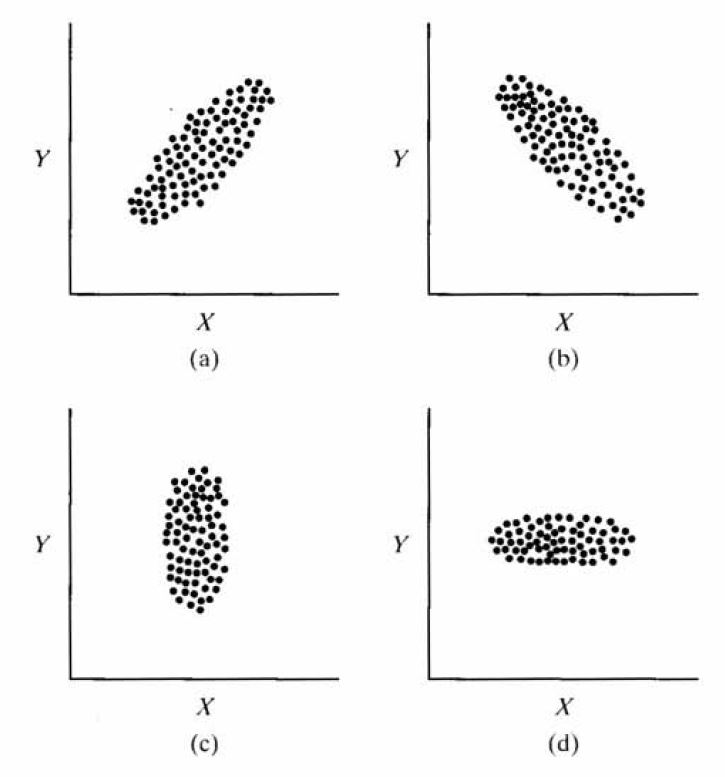
\includegraphics[width=\textwidth]{figures/dHTAanalyse/r_vaerdi}
\caption{Figuren illustrerer forskellige muligheder for korrelation mellem to datasæt. For disse grafer er Y det afhængige datasæt, mens X er uafhængig. Graf (a) illustrerer en positiv korrelation mellem X og Y, hvormed R-værdien er lig 1. På graf (b) vises negativ korrelation mellem X og Y, med en R-værdi på -1. For graf (c) og (d) er R-værdien 0, og der er dermed ingen korrelation mellem X og Y. \textit{Fra \citer{Zar2010}}}\label{fig:r_vaerdi}
\end{figure}

Som det ses ud fra \figref{fig:r_vaerdi} er der større korrelation mellem to datasæt jo tættere på 1 |R| kommer. Hermed bestræber studier, der finder en statistisk sammenhæng mellem to datasæt, sig på, at den numeriske værdi af R for sammenhængen er så tæt på 1 som muligt. Styrken af sammenhængen mellem to datasæt ud fra R-værdien kan ses i \tabref{tab:styrke_r}. \\

\begin{table}[H]
\centering
\begin{tabular}{cc}
\rowcolor[HTML]{C0C0C0} 
R-værdi {[}numerisk{]} & Betydning  \\ \hline
0,9 til 1              & Meget høj korrelation              \\
0,7 til 0,9            & Høj korrelation                    \\
0,5 til 0,7            & Moderat korrelation                \\
0,3 til 0,5            & Lav korrelation                    \\
0 til 0,3              & Ingen korrelation                  \\ \hline
\end{tabular}
\caption{Tabellen viser betydningen af forskellige R-værdier. R-værdierne er angivet som numeriske værdier, hvormed betydningen af værdierne gælder for både positive og negative korrelationer. \textit{Tabellen er modificereret fra \citer{Mukaka2012}}}
\label{tab:styrke_r}
\end{table}

Flere studier som har fundet en statistisk signifikant sammenhæng mellem en af det tre QST-parametre, har ligeledes undersøgt R-værdien for denne sammenhæng. For et studie af \citer{Wylde2013} blev der fundet en statisk signifikant sammenhæng mellem præoperativ PPT-resultater og udviklingen af kroniske postoperative smerter med en p-værdi på 0,008. Korrelationskoefficienten for denne sammenhæng blev fundet til 0,37. Hermed er sammenhængen mellem præoperativ PPT-resultater og kroniske postoperative smerter lav, og næsten i en størrelsesorden hvor der ingen korrelation er (jævnfør \tabref{styrke_r}). Denne lave R-værdi er en tendens der er generel for studier, der har fundet en statistisk signifikant sammenhæng mellem en af de tre QST parametre og kroniske postoperative smerter. Eksempelvis er R-værdien for studiet af \citer{Petersen2016}, hvor der findes en sammenhæng mellem præoperativ PPT og postoperativ smertelindring, på -0,216. Udfra \tabref{tab:styrke_r} indikerer denne R-værdi at der ikke er nogen korrelation imellem de to datasæt. Ligeledes er R-værdien fra et studie af \citer{Petersen2015} for sammenhængen mellem TSP og postoperativ kronisk smerte på 0,24. Heller ikke denne R-værdi viser en korrelation. \\
Det at ingen af de undersøgte studier har vist en korrelation der er mere end lav, antyder at den individuelle linære sammenhæng mellem de tre QST-parametre og kroniske postoperative smerter er dårlig. Det er i studiet af \citer{Petersen2016} ikke undersøgt korrelationen mellem faciliteret TSP og mindsket CPM sammen og postoperative kroniske smerter, men dette vil kunne gøres ved anvendelse af en mutibel regressionsanlyse.  

\subsubsection{Sensitivitet og specificitet}
For at en kliniker vil kunne anvende QST-parametrene til at fænotypebestemmme patienter med knæartrose, er det nødvendigt for klinikeren at vide hvor specifik og sensitiv QST-undersøgelserne er. Specificitet og sensitivitet siger noget om hvor god en undersøgelse er til at finde sande negative og sande positive patienter. Fremadrettet betegnes positive resultater som resultater der er anormale. Dette vil sige at et positivt resultat for PPT er en lav PPT-værdi, mens det for TSP er en høj TSP-værdi og for CPM er en lav CPM-værdi \citep{Petersen2016}. Hermed vil en patient som har et positivt resultat af undersøgelserne være centralt sensibiliseret. \\
Resultater fra en undersøgelse kan opdeles i fire kategorier; sande positive (SP), falske positive (FP), sande negative (SN) og falske negative (FN). Disse fire resultater er illustreret i \tabref{tab:pos_neg}.

\begin{table}[]
\centering
\begin{tabular}{llcc}
\rowcolor[HTML]{C0C0C0} 
\cellcolor[HTML]{C0C0C0}                                 &         & \multicolumn{2}{c}{\cellcolor[HTML]{C0C0C0}Sygdom}        \\ \cline{2-4} 
\cellcolor[HTML]{C0C0C0}                                 &         & \multicolumn{1}{l}{Positiv} & \multicolumn{1}{l}{Negativ} \\
\cellcolor[HTML]{C0C0C0}                                 & Positiv & Sand positiv                & Falsk positiv               \\
\multirow{-4}{*}{\cellcolor[HTML]{C0C0C0}Testresultater} & Negativ & Falsk negativ               & Sand negativ               
\end{tabular}
\caption{Tabellen viser de fire mulige resultater fra en undersøgelse. \textit{Modificeret fra \citer{Parikh2008}}}
\label{tab:pos_neg}
\end{table}

Som det ses ud fra \tabref{tab:pos_neg} kan undersøgelser vise både falsk positive og falsk negative resultater. Disse falske resultater er problematiske, idet resultaterne betyder patienten risikerer at få den forkerte behandling \citep{Lalkhen2008}. For knæartrosepatienter vil falsk positive resultater betyde at patienten ikke vil blive tilbudt en TKA-operation, selvom denne ikke har central sensibilisering. Ligeledes vil falsk negative resultater betyde at en patient med central sensibilisering vil få en TKA-operation, hvorefter denne patient har betydeligt større risiko for at udvikle kroniske smerter end andre patienter. En undersøgelses sensitivitet og specificitet kan anvendes til at undersøge risikoen for falske resultater. \\
Den matematiske definition af sensitivitet er: \\
$Sensitvitet=\frac{SP}{SP+FN}$ \\
Herudfra kan det ses at sensitiviteten af en undersøgelse vil stige når antallet af falske negative resultater falder. En undersøgelse med en sensitivitet på 100\% vil korrekt identificere alle patienter med sygdommen. Hvis undersøgelsen har en sensitivitet på mindre end 100\% vil en del af de patienter som har sygdommen, have falsk negative resultater og hermed blive fejldiagnosticeret. Sensitivitet er dermed et udtryk for hvor stor en andel af patienterne med en sygdom undersøgelsen er i stand til at opfange. \citep{Lalkhen2008} \\
Specificitet er det modsatte af sensitivitet, hvilket vil sige en undersøgelses specificitet er et udtryk for hvor mange patienter som ikke har sygdommen undersøgelsen korrekt vil være i stand til at identificere \citep{Lalkhen2008}. Den matematiske definition på specificitet er: \\
$Specificitet=\frac{SN}{SN+FP}$ \\
Dette betyder at en undersøgelses specificitet stiger når antallet af falske positive resultater falder. \citep{Lalkhen2008} \\
Ideelt set vil en undersøgelse have både en sensitivitet og specificitet på 100\%, hvormed undersøgelsen altid vil identificere patienter med sygdommen som positive og patienter uden sygdommen som negative. Denne type undersøgelse er i de fleste tilfælde urealistisk, hvormed det kan være nødvendigt at lave et kompromis mellem sensitivitet og specificitet. Dette betyder at en undersøgelse med en høj sensitivitet vil have en lav specificitet, og omvendt for en undersøgelse med en høj specificitet. Om en undersøgelse skal have en høj sensitivitet eller en høj specificitet afhænger af sygdommen der undersøges for, og de etiske konsekvenser for hver af de to falske resultater (dette undersøges nærmere for QST-undersøgelser i \chapref{chap_EFF}).  \\
Der er på nuværende tidspunkt ikke publiceret data omkring sensitiviteten og specificiteten for QST-undersøgelserne. \citep{Wylde2013} Disse data er essentielle for om QST-undersøgelserne kan anvendes som supplement til klinikerens vurderingsgrundlag, idet det ud fra sensitiviteten og specificiteten kan vurderes hvor stor vægt klinikeren skal lægge i resultater fra undersøgelserne. På \figref{fig:AUC} illustreres tre muligheder for sensitivitet og specificitet:

\begin{figure}[H]
\centering
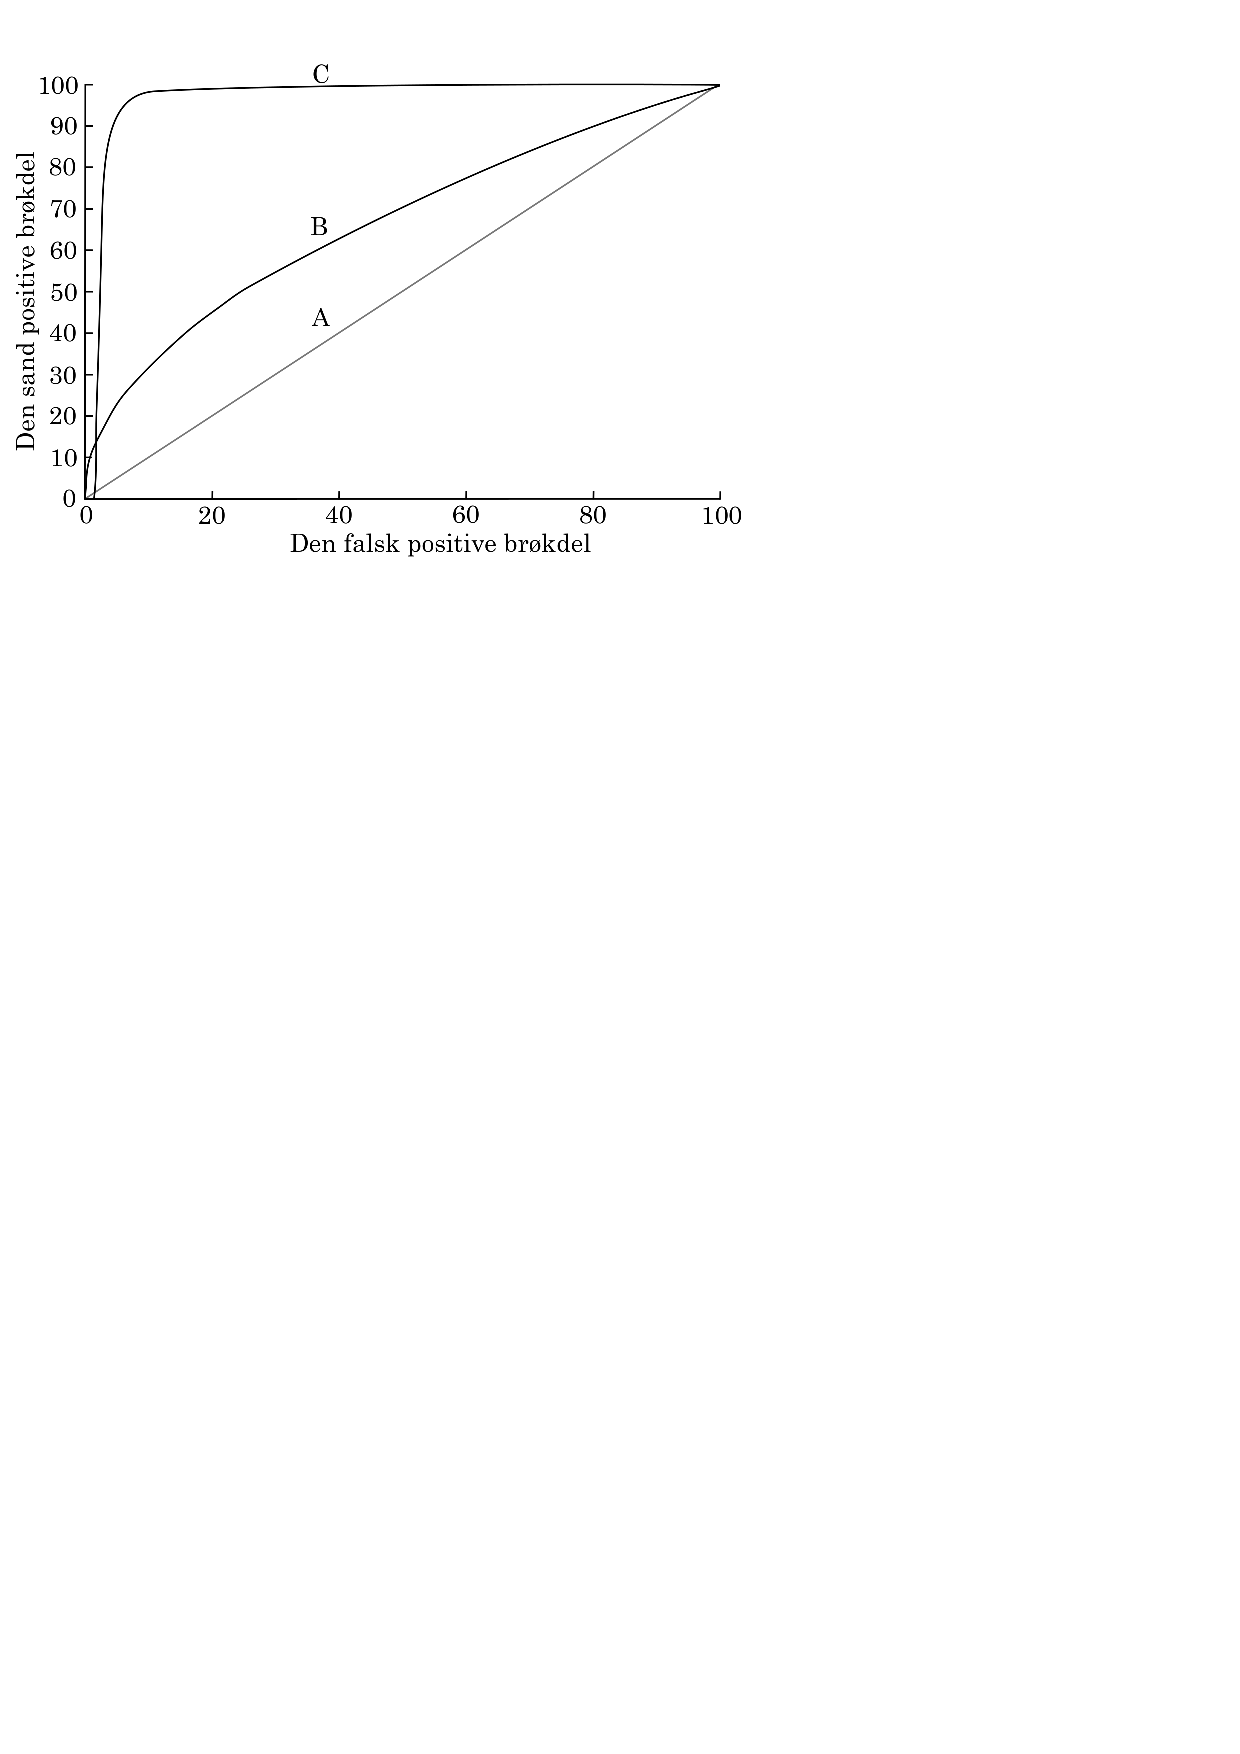
\includegraphics[width=\textwidth]{figures/dHTAanalyse/AUC}
\caption{Figuren illustrerer tre mulige sammenhænge mellem sensitivitet og specificitet, når cut-off værdien for undersøgelsen ændres. Op af y-aksen er den sande positive brøkdel (sensitiviteten) angivet, mens den falske positive brøkdel (100-specificiteten) er hen ad x-aksen. Linje C viser plottet for en ideel undersøgelse, mens linje B viser det typiske plot for en undersøgelse som anvendes normalt i klinisk praksis. Den stiplede linje, A, viser linjen for nul diskrimination. \textit{Fra \citer{Lalkhen2008}}}\label{fig:AUC}
\end{figure}

Den stiplede linje, A, som vises på \figref{fig:AUC}, angiver linjen for nul diskrimination. Dette betyder at undersøgelser hvis plot ligger på denne linje ikke kan skelne mellem sande positive og sande negative, og resultater fra undersøgelsen har 50\% risiko for at være forkerte. Arealerne under kurverne angiver præcisionen for en undersøgelse, hvor en ideel undersøgelse (linje C) har et areal under kurven på 1 mens nul diskriminationslinjen (linje A) har et areal under kurven på 0,5. \\
Udfra dette vil QST-undersøgelserne, før disse kan være anvendelige for en kliniker, skulle have en præcision der er højere end 0,5 og så tæt på 1 som muligt. Hvis QST-undersøgelserne ikke har denne præcision vil disse være svære for klinikeren at anvende, hvormed det er nødvendigt at undersøge sensitivitet og specificitet for undersøgelserne.   

\section{Nøjagtighed}
\textit{I følgende afsnit vil QST-undersøgelsernes nøjagtighed blive beskrevet, både i dets resultater, men også i forhold til teknologiens relibilitet. Dette er for at kunne vurdere egentheden af QST-undersøgelserne, som et brugbart supplement.}

\subsection{Patientgruppering på baggrund af QST-resultater}
Det forsøges at skabe en præoperativ smerteprofil som indikerer hvorvidt en patient er disponeret for at udvikle kroniske postoperative smerter. Som nævnt i \secref{TEC} er der en indikation på at nedsat PPT, forhøjet TSP og nedsat CPM er de diagnostisk relevante QST-parametre, til at kunne skabe den omtalte smerteprofil. \\
Studiet af \citer{Suokas2012} har undersøgt forskellige studiers PPT-resultater opnået igennem, raske kontrolgrupper og grupper som lider af knæartrose. PPT-resultatet heraf er gennemsnittet og stammer fra forskellige anatomiske placeringer, eksempelvis, på det påvirkede knæ, under det påvirkede knæ samt væk fra det påvirkede knæ. Patientgruppen som lider af knæartrose, opnåede følgende PPT resultater, 177 kPa ($\pm$ 98) til 512 kPa ($\pm$ 221), hvilket var lavere end hos den raske kontrolgruppe. Den raske kontrolgruppe opnåede resultaterne imellem 333 kPa ($\pm$ 82) og 1098 kPa ($\pm$ 199). \citep{Suokas2012} Denne indikation er ligeledes påvist i studiet af \citer{Wylde2013}, som testede PPT på det påvirkede knæ, samt på underarmen. De raske forsøgspersoner opnåede i gennemsnit PPT-resultater på henholdsvis 405 kPa på knæet og 339 kPa på underarmen. Knæartrosepatienterne havde som i studiet af \citer{Suokas2012}, ligeledes lavere PPT-resultater end de raske. PPT-resultaterne var henholdsvis 155 kPa på knæet og 171 kPa på underarmen. \citep{Wylde2013} 

\begin{table}[H]
	\centering
	\resizebox{\textwidth}{!}{%
		\begin{tabular}{ccc}
			\hline
			\rowcolor[HTML]{C0C0C0} 
			Studie               & Kontrol patientgruppe: PPT {[}kPa{]} & Knæartrose patientgruppe: PPT {[}kPa{]} \\ \hline
			\citer{Suokas2012} & 333 ($\pm$ 82) til 1098 ($\pm$ 199)      & 177 ($\pm$ 98) til 512 ($\pm$ 221)          \\
			\citer{Wylde2013}  & 405 (knæ) og 339 (underarmen)        & 155 (knæ) og 171 (underarmen)           \\ \hline
		\end{tabular}
	}
	\caption{I tabellen ses resultaterne vedrørende PPT-målinger på henholdsvis raske person og knæartrsoe patienter.  }
	\label{tab:PPT_rask_syg}
\end{table}\vspace{-.25cm}
Resultaterne præsenteret i studiet \citer{Suokas2012} og \citer{Wylde2013}, som ses i \tabref{tab:PPT_rask_syg}, viser at der imellem raske og knæartrosepatienter er en signifikant forskel af PPT-resultater. Der ses heraf en tendens til at knæartrosepatienterne kan modstå mindre tryk førend sensationen af stimuliet opfattes som værende smerte, end raske personer.

QST bliver ligeledes benyttet af \citer{Petersen2015} og \citer{Wright2015}, men til at undersøge forskellen af PPT-resultater knæartrosepatienter imellem. \citer{Wright2015} inddelte patienterne som havde undergået TKA i grupperinger; en gruppering med moderat til kraftig smerte(Gruppe A) og en gruppering uden smerter (Gruppe B). Gruppe A havde gennemsnitligt PPT resultater henholdsvis ved knæet på 282 kPa og ved den distale albue på 314 kPa. Gruppe B havde gennemsnitligt PPT-resultater ved knæet på 416 kPa og ved den distale albue på 454 kPa. Studiet af \citer{Petersen2015} vidste ikke samme grad af spredning i resultaterne imellem grupperingen med høje og lave kroniske postoperativ smerte, men vidste ligeledes samme tendens grupperingerne imellem. Grupperingen med lave kroniske postoperative smerter havde omtrent et PPT-resultat ved det påvirkede knæ på 600 $\pm$ 25 kPa, og på armen omkring 460 $\pm$ 10 kPa. Grupperingen med høje kroniske postoperative smerter havde omtrent et PPT-resultat ved det påvirkede knæ på 550 $\pm$ 50 kPa, og på armen 460 $\pm$ 20 kPa. \citep{Petersen2015}

\begin{table}[H]
	\centering
	\resizebox{\textwidth}{!}{%
		\begin{tabular}{ccc}
			\hline
			\rowcolor[HTML]{C0C0C0} 
			Studie                 & Lav smerte gruppe: PPT {[}kPa{]}     & Høj smerte gruppe: PPT {[}kPa{]}     \\ \hline
			\citer{Wright2015}   & 416 (knæ) og 454 (albue)             & 282 (knæ) og 314 (albue)             \\
			\citer{Petersen2015} & 600 $\pm$ 25 (knæ) og 460 $\pm$ 10 (arm) & 550 $\pm$ 50 (knæ) og 460 $\pm$ 20 (arm) \\ \hline
		\end{tabular}
	}
	\caption{I tabellen ses resultaterne vedrørende PPT-målinger på henholdsvis en gruppering med lave og høje kroniske postoperative smerter.}
	\label{tab:PPT_syg_syg}
\end{table}\vspace{-.25cm}
Resultaterne præsenteret i studiet \citer{Wright2015} og \citer{Petersen2015}, som ses i \tabref{tab:PPT_syg_syg}, viser at der blandt knæartrosepatienter med forskellige grad af kronisk postoperativ smerter, er en forskel i deres PPT-resultater. På baggrund af resultaterne opnår knæartrosepatienter med høje kroniske postoperative smerter, lavere PPT-resultater, end grupperingen med lave kroniske postoperative smerter. \citep{Wright2015} \citep{Petersen2015}

I studiet af \citer{Vaegter2016} undersøges forskellige smertemoduleringers egenskaber til at kunne danne patientgrupperingen vedrørende kroniske smerter. Studiet undersøger påvirkningen af QST-parametrene TSP og CPM, på kroniske smertepatienter. Resultaterne fra studiet viser at de kvindelige patienter med nedsat CPM faldt -11,6 $\pm$ 19,3 \% fra det først målte PPT-resultat, og at de mandlige patienter med nedsat CPM faldt -3.6 $\pm$ 17 \% fra det først målte PPT-resultat. Studiets resultater vedrørende TSP blev opgivet i en VAS ratio for VAS3 over VAS1. VAS3 bestod af gennemsnittet af [8,9] stimuli respons og VAS1 bestod af gennemsnittet af [1,..,4] stimuli respons. Resultaterne for både de kvindelige og mandelige patienter med faciliteret TSP var en VAS-ratio på 1,7 $\pm$ 0,4. Faciliteret TSP og nedsat CPM er påvist at kunne prædiktere kroniske smerte hos patienter der har gennemgået torakotomi og abdominal kirurgi. \citep{Vaegter2016} \\
Studier af \citer{Petersen2016} og \citer{Petersen2015} er det undersøgt hvordan TSP og CPM har indflydelse på en patients kroniske postoperative smerter. I studiet af \citer{Petersen2016} blev det bekræftet at patienter med faciliteret TSP og nedsat CPM var den patientgruppering med fleste kroniske postoperative smerter. I studiet blev det arbitrært bestemt at faciliteteret TSP var resultater over gennemsnittet, og at nedsat CPM var resultater under gennemsnit. CPM blev i studiet bestemt ved at trække PPT-resultat fra CPM-målingen fra det målte PPT-resultat forud for testen, og var gennemsnitligt 5,40 $\pm$ 1,05 kPa. Grupperingen med nedsat CPM havde gennemsnitligt resultatet -2 $\pm$ 0,5 kPa. TSP blev i studiet bestemt ved at trække VAS2 som værende gennemsnittet af måling [8,..,10] fra VAS1 som værende gennemsnitet af måling [1,..,4] og var 1,55 $\pm$ 0,17. Grupperingen med faciliteret TSP havde gennemsnitligt resultatet 3 $\pm$ 0,5. 

\begin{table}[H]
	\centering
	\resizebox{\textwidth}{!}{%
		\begin{tabular}{ccc}
			\hline
			\rowcolor[HTML]{C0C0C0} 
			Studie                 & Gruppering med nedsat CPM                                                                   & Gruppering med faciliteret TSP \\ \hline
			\citer{Vaegter2016}  & \begin{tabular}[c]{@{}c@{}}-11,6 $\pm$ 19,3 \% (kvinder)\\ -3.6 $\pm$ 17 \% (mænd)\end{tabular} & 1,7 $\pm$ 0,4 (kvinder og mænd)  \\
			\citer{Petersen2016} & -2 $\pm$ 0,5 kPa                                                                              & 3 $\pm$ 0,5                      \\ \hline
		\end{tabular}
	}
	\caption{I tabellen ses resultaterne vedrørende CPM og TSP målinger på gruppering med nedsat CPM og faciliteret TSP.}
	\label{tab:CPM_TSP}
\end{table}

Resultaterne præsenteret i studiet \citer{Veagter2016} og \citer{Petersen2016}, som ses i \tabref{tab:CPM_TSP }, viser at kroniske smertepatienter har nedsat CPM og faciliteret TSP. Det påvises i studierne at patienter med disse tilstand har signifikant flere kroniske smerter. \citep{Veagter2016} \citep{Petersen2016}

Ovenstående resultater omhandlende patientgruppering for QST-parametrene PPT, TSP og CPM varerier tydeligt. Det ses af resultaterne at det er muligt ved benyttelse af QST, at se forskel på patienter uden central sensibilisering og patienter med. Det kan yderligere ses på resultaterne at der imellem de forskellige studiers resultater ikke er nogen eksakt konsistens, de viser dog samme tendens. Dette kan være en indikation for forskelligt anvendt udstyr, samt undersøgelsens metode. Herfor skal man udføre QST ens alle gange og med samme udstyr før det giver mening at lave et normativt datasæt. Et normativt datasæt til inddeling af patienter i grupperinger, med tilhørende udførelig metode til undersøgelsen, skal udarbejdes førend patienter kan klassificeres som værende i en anormal tilstand.  Ovenstående indikerer, at resultaterne for PPT, TSP og CPM varierer imellem knæartrosepatienter, og at disponerede patienter for kroniske postoperative smerter har lavere PPT, faciliteret TSP og nedsat CPM. 

\subsection{Repeterbarhed for QST}
I et studie af \citer{Nielsen2015} er repeterbarheden for manuelt udførte PPT-undersøgelser blevet undersøgt. De 136 forsøgspersoner, der indgik i studiet, blev undersøgt ved brug af et trykalgometer fra Somedic. Forsøget blev udført på låret (quadriceps) og på overarmen (biceps brachii) i forsøgspersonernes dominante side. Studiet var struktureret i to sessioner med minimum en uges mellemrum. Forsøgets resultater viste, at inter-korrelations koefficienten (ICC) mellem de målte data for de to sessioner var 0,89 for ben og 0,87 arme. Begge disse værdier er i studiet defineret som værende høje, da de overskrider den fastsatte tærskelværdi på 0,75. Analysen af resultaterne viste endvidere en bias både for ben og arme i form af en forskel mellem de beregnede middelværdier for de to sessioner. Det samme studie undersøgte repeterbarheden for PPT-undersøgelser udført med computerstyret cuff-algometri. Til denne undersøgelse blev et cuff-algometer fra Nocitech placeret henholdsvis omkring læggen og overarmen i den non-dominante side. Forsøgspersonerne skulle under forsøget kvantificere deres smerte ved hjælp af en elektronisk VAS-tabel. Når smerten blev uudholdelig skulle forsøgspersonerne selv trykke på en knap, der stoppede trykpåvirkningen i cuff-algometeret, hvorefter forsøget var afsluttet. Resultaterne viste en interkorrelationskoefficient på 0,79 for benet og 0,85 for armen, hvilket igen i dette studie er defineret som høje korrelationer. Ligesom for den manuelle PPT-undersøgelse viste dette forsøg en systemisk fejl mellem de to sessioner, men kun for målingerne på armen.

I et litteraturstudie af \citer{Kennedy2016} blev repeterbarheden for CPM-undersøgelser på forskellige områder af kroppen analyseret. Analysen var baseret på 10 studier, hvoraf fem studier anvendte PPT som teststimuli. Typen af konditionerede stimuli varierede imellem de fem studier. I et studie blev den opfølgende test lavet under samme session som den primære, imens der i tre andre studier blev udført en opfølgende test i løbet af to til ti dage. I det sidste studie blev der både foretaget en opfølgende test i samme session som den primære og yderligere en opfølgning tre dage senere. \citer{Kennedy2016} opdelte studiernes resultater i henholdsvis repeterbarhed for teststimuli og for konditioneret stimuli. Det fremgår, for forsøgene, hvor den opfølgende test er udført i samme session som den primære, at ICC ligger på 0,82-0,87 for teststimuli (PPT), hvilket overskrider grænsen for høj korrelation på 0,75. For studierne, der har afholdt to uafhængige sessioner ligger ICC i intervallet 0,65-0,79 og defineres derfor som værende god til høj. For de konditionerede stimuli, hvor den opfølgende test blev lavet i samme session som den primære, lå ICC på 0,60-0,94. For studierne, der udførte den opfølgende test i en separat session var ICC i intervallet 0,61-0,82.\\ 
Et studie af \citer{Imai2016} undersøgte ligeledes, hvordan CPM-undersøgelsers repeterbarhed påvirkes ved ændring af test- og konditionerede stimuli. I studiet indgik 26 raske mænd. Hver forsøgsperson gennemgik to identiske sessioner med højst 3 ugers mellemrum. Der blev anvendt fire forskellige typer teststimuli, hvoraf de to var baseret på tryk (manuel- og cuff-algometri). Trykket blev påført med et algometer fra Somedic og en cuff fra Nocitech. Både det håndholdte og cuff-algometeret var placeret på underbenet ved forsøgene. Den konditionerede stimuli blev påført kontralateralt for teststimuli og var udgjort af cold pressor threshold (CPT) og cuff-algometeret. I studiet er ICC-værdierne for forsøgene med trykbaseret teststimuli henholdsvis 0,49 og 0,44 for CPT, mens de for cuff-algometri er 0,04 og 0,53.\\ 
I studiet af \citer{Nielsen2015} blev TSP undersøgt i forlængelse af de cuffbaserede tests af PPT og smertetolerance (PTT). Undersøgelsen foregik ved at cuff-algometeret blev pustet op til et tryk svarende til den fundne smertetolerance 10 gange af to sekunders varighed. Resultaterne for studiet viste en ICC på 0,60 for benet og 0,43 for armen. 

Flere studier har undersøgt repeterbarheden for udførelsen af PPT- TSP- og CPM-undersøgelser. På baggrund af resultaterne kan det ses, at der generelt forekommer en høj ICC for PPT-undersøgelser baseret på de definerede tærskelværdier i de respektive studier. For CPM-undersøgelser forekommer der generelt en større variation i resultaterne. ICC-værdierne for TSP fundet af \citer{Nielsen2015} er i intervallet middel til god, men dette resultat kan med fordel underbygges af flere studier. 

%% Skal vi nævne at Cuffen er udviklet af AAU
Det er ligeledes væsentligt for vurderingen af den samlede behandling, hvilke tiltag der er mulige, og hvor stor effekten er af disse, hvis QST kan identificere patienter som har en forhøjet risiko for at udvikle kronisk smerte efter en TKA-operation.

\section{Delkonklusion}
Det er af væsentlig betydning at tage i betragtning, at de fundne studier har undersøgt virkningsgraden for QST under forskningsmæssige forhold. Flere af de undersøgte studier har vist, at der statistisk set er en sammenhæng mellem de undersøgte prædiktorer, og kroniske smerte efter TKA-operation. Det er dog karakteristisk for studierne, at der foreligger divergerende resultater, og at der generelt er en ringe korrelation mellem de undersøgte parametre og forekomst af kronisk smerte efter TKA-operation. Det har heller ikke være muligt, at opspore konkrete tal i forhold til specificitet og sensitivitet, i forhold til at kunne vurdere den kliniske effekt af QST, og dermed kunne vurdere det diagnostiske potentiale for teknologien. Dette skal betragtes i lyset af manglen på egentlige tærskelværdier for hvornår man definerer en patient som en kronisk smerte patient, men også for hvorledes man definerer en patient til at have faciliteret TSP eller svækket CPM. Det giver også anledning til bekymring, i forhold til i hvor høj grad resultaterne kan overføres fra forskningsregi til daglig praksis.
I denne analyse blev der generelt fundet en god repeterbarhed for måling af PPT. Resultaterne for TSP- og CPM-parametrene havde dog en højere grad af spredning i resultaterne.
Det er dog essentielt at understrege, at QST i forhold til prædiktion af kronisk postoperativ smerte, er en teknologi der stadig er under afprøvning og udvikling, og de lovende indikationer som er vist i studierne skal replikeres for at kunne cementere den kliniske effektivitet af QST.


















%\section{Effekt og skade}
%\textit{I følgende afsnit undersøges, den samlede effekt af behandlingen, hvori QST er tiltænkt at indgå. QST er kun et delelement i patientens behandling og derfor er en vurdering af isolereret vurdering af QST-teknologien ikke tilstrækkelig.\fxnote{Den her argumentation kan jeg slet ikke følge - det giver da mening at se på effekten af QST alene}. Svar: tanken var lidt, at man kan f.eks. også kan screene for diabetes 1 lang tid før sygdommen optræder, men dette har ikke nogen stor værdi, da man alligevel ikke kan gøre for at forhindre at sygdommen kommer alligevel. At kunne screene nogle patienter man alligevel ikke kan hjælpe, har vel ikke så meget værdi, set ud fra et patientperspektiv - medmindre man kan forhindre de kroniske smerter.}
%
%\subsection{Gavnlige effekter ved QST} \fxnote{Jeg kan ikke se sammenhængen mellem det her og spørgsmålet - og slet ikke argumentationen for kun at fokusere på medicin og ikke selve QST-undersøgelserne. Svar: }
%Ved at kunne prædiktere om patienten får kroniske smerter, kan patienterne informeres om den mulige forhøjede risiko for at opleve kroniske smerter, som der kan være forbundet med en TKA-operation. Patienten kan således informeres om, at medicinsk behandling kan reducere risikofaktorer for udvikling af kroniske postoperative smerte.%, herunder TSP og CPM. 
%For eksempel er NMDA antagonisten, Pregabalin, blevet foreslået til at reducere kronisk smerte som følge af TKA. Der er dog ikke et entydigt resultat af, hvor stor denne effekt er. \citer{Lunn2015a} har i et studie med 300 patienter undersøgt effekten af Gabapentin, hvor der ikke blev fundet en signifikant forskel mellem placebogruppen og gruppen der fik medicin. Dette står dog i kontrast til et andet studie af \citer{Buvanendran2010}, som med 120 forsøgspersoner viser at der var en signifikant effekt ved medicnsk behandling med Pregabalin. 
%Det optimale udbytte af den samlede diagnosticering og behandling, er at patienten ikke oplever kronisk smerte efter en TKA-operation. %\citer{Kristensen2015} har i et studie med 215 primære TKA-patienter vist at kronisk smerte 3 år efter operationen har en sammenhhæng med Knee Society Score (KSS) som er en funktionsscore der afspejler patientens knæfunktionalitet.
%
%\fxnote{Der mangler et afsnit om net-benefit!}
%
%
%
%\subsection{Klinisk effekt}
%For at vurdere hvor nøjagtig QST er, benyttes data fra studier der har undersøgt kronisk smerte efter en TKA. Kronisk smerte defineres som smerte der rækker ud over den normale vævshelingsperiode. I forhold til TKA-patienter kan denne periode vare i op til 12 måneder \citep{Wylde2015}. Derfor vil de inkluderede studier også benytte denne minimumsperiode som referencepunkt. \\
%%Under litteratursøgningen blev 6 studier fundet relevante. Disse er i det følgende beskrevet i kronologisk rækkefølge.
%
%\citer{Wylde2013} undersøgte forholdet mellem præoperative smertetærskler hos TKA patienter og disse patienters oplevelse af smerte 12 måneder efter TKA-operationen. I studiet deltog 51 patienter der var indstillet til TKA. Disse fik målt deres smerteintensitet ved hjælp af WOMAC (Western Ontario and McMaster Universities Osteoarthritis Pain scale). Denne smertetest tager gangsmerter, smerte ved brug af trapper, smerter i siddende eller liggende position og smerter ved stående position, i betragtning. \fxnote{Kilde?} I studiet blev blandt andet PPT målt. Disse målinger blev sammenlignet med målinger på 50 personer uden knæsmerter. I studiet blev der fundet en signifikant korrelation mellem præoperativ lav PPT, målt på underarmen og øget smerte 12 måneder efter TKA-operationen.
%
%Wylde et al, 2014 har i et dobbeltblindet, randomiseret single-center studie med 239 patienter, undersøgt om PPT målt på underarmen kunne prædiktere om patienter ville komme til at opleve smerte 12 måneder efter operationen. Smerten blev vurderet ud fra WOMAC smertescoren. Det blev fundet at lav PPT korrelerede i forhold til patientens oplevelse af præoperativ smerteintensitet. Derudover blev det fundet at PPT ikke kunne prædiktere niveauet af smertelindring efter TKA-operation, uafhængigt af præoperativ smerteintensitet.
%
%Wright et al, 2014 har i et studie undersøgt om der eksisterede en sammenhæng i forhold til målt PPT hos 53 TKA-patienter som rapporterede henholdsvis moderat til svær smerte eller ingen smerte, 12 måneder efter TKA-operation. Til at måle PPT blev et algometer med $1 cm^{2}$ probe anvendt (Somedic,Sverige). I studiet blev det fundet at patienter med moderat til svær smerte havde reduceret PPT ved knæet.
%
%\citer{Petersen2015} har i et studie undersøgt korrelation mellem PPT, TSP og CPM i forhold til udvikling af kronisk smerte efter TKA-operation. Smerteintensiteten blev målt ved hjælp af VAS, og de tre parametre blev målt henholdsvis før operationen, 2 måneder efter operationen og 12 måneder efter operationen. Patienterne blev opdelt i en gruppe med lav smerte (VAS < 3) (N=61) og en gruppe med høj smerte (VAS>=3) (N=17). Inddelingen var baseret på smerten hos patienten 12 måneder efter TKA-operation. Petersen fandt at præoperativt PPT ikke kunne prædiktere smerte 12 måneder efter operationen. \\ % En von Frey stimulator blev benyttet til at inducere TSP. Smerten blev induceret tæt på det afficerede led. Stimulationen blev påført 10 gange efter hinanden. TSP blev defineret som forskellen i intensiteten mellem første og sidste stimulation. CPM blev defineret som forskellen i PPT før og efter den betingede stimulation. Til at inducere den toniske stimulation blev den kontralaterale hånd i forhold til det afficerede knæ nedsænket i isvand.\\ 
%Studiet fandt at TSP med 25.6 gram mekanisk stimulus på det afficerede knæ var relateret til smerte 12 månender efter operationen. I studiet havde gruppen med høj smerte efter 12 måneder, også en højere smerteintensitet før operationen sammenlignet med gruppen med lav-intensitet smerte (P=0.009) 12 måneder efter operationen (P < 0.001). Studiet viste også at PPT-målingerne for lavsmerte gruppen blev normaliserede efter operation (P<0.05). For gruppen med høj smerte efter 12 måneder var præoperativ TSP korreleret til smerte 12 måneder efter operationen (R=0.240, P =0.037).
%Studiet viste at der var en positiv korrelation mellem 12 måneders postoperativ smerte intensitet, preoperativt smerteintensitet (R=0.229, P=0.045) og præoperativ TSP (R=0.240, P=0.037). Ingen korrelation blev fundet mellem PPT og postoperativ smerte 12 måneder efter operationen. Derudover var der ikke en korrelation mellem CPM og post-operativ smerte 12 måneder efter operationen. \citep{Petersen2015}
%
%\citer{Petersen2016} har i et single center  studie undersøgt post-operativ smertelindring 12 måneder efter TKA-operation. I studiet deltog 103 patienter. Patienterne blev profilerede og derefter opdelt i 4 undergrupper før TKA-operationen. Disse var henholdsvis a)  Faciliteret TSP/nedsat CPM (N=16), b) Faciliteret TSP/normal CPM (N=15), c)  Normal TSP/nedsat CPM ( N=44), d) Normal TSP/normal CPM. Der blev benyttet et computerstyret cuff-algometer og en elektronisk VAS-måleenhed. I studiet blev en række parametre målt; TSP, CPM, PDT, PTT og PPT. \\
%\citer{Petersen2016} fandt, at en lav PDT var associeret med en mindre postoperativ smertelindring (R=-0.222, P=0.034). Derudover blev der fundet en sammenhæng mellem præoperativ smerte og postoperativ smertelindring (R=0.263, P=0.080).
%Hverken faciliteret TSP eller nedsat CPM alene, kunne påvise en signifikant sammenhæng i forhold til smerte 12 måneder efter TKA-operation. Studiet viste derudover, at gruppen med faciliteret TSP sammen med nedsat CPM (gruppe a) var den gruppe der oplevede mindst smertelindring.
%Disse resultater kan indikere, at gruppe a har mindre sandsynlighed for at opleve en smertelindring.\\
%Det er vigtigt at påpege at dette studie er en eksplorativ undersøgelse, og dette indebærer også at der ikke blev udarbejdet en plan på forhånd, for hvorledes de statistiske udregninger skulle udføres.
%Derudover nævner forfatteren at studiet ikke var designet til at prædiktere, hvilke patienter der ville udvikle kroniske smerter. \citep{Petersen2016}
%
%Wylde, 2016 har i et studie undersøgt sammenhængen mellem præ-operativ udbredt hyperalgesi og graden af radiografisk artrose, i forhold til smertegrad før en TKA og 12 måneder efter. I studiet deltog 241 TKA-patienter. Smerten blev vurderet ud fra WOMAC-skalaen. Den radiografiske artrose blev vurderet ud fra Kellgren og Lawrence skalaen, som vurderer sværhedsgraden fra 0-4, hvor 4 er sværest. Den udbredte hyperalgesi blev målt ved hjælp af algometer med $1 cm^{2}$ probe (Somedic, sverige) ved måling af PPT på underarmen.
%I studiet blev der fundet en signifikant korrelation mellem radiografisk artrosesværhedsgrad og postoperativ smerteintensitet. Derudover var højere PPT signifikant associeret med mindre præoperativ smerte.	
%\fxnote{Hvor er sammenligningen mellem studierne - analysedelen af det her afsnit mangler. Hvorfor er de her studier relevante, hvordan hænger de sammen, og hvad siger de om forskellen mellem kronisk smerte og ikke-kronisk smerte patienter? Der bliver heller ikke her svaret på spørgsmålet}






\chapter{Omkostninger og økonomisk evaluering (ECO)}\vspace{-.75cm} \label{ECO_chap}
\section{Formål}
I dette domæne undersøges det hvilke økonomiske konsekvenser der vil opstå ved implementering og brug af QST-protokollen. Ved implementering af QST-protokollen forventes det, at der vil være omkostninger i forhold til indkøb, personel og drift. Disse økonomiske omkostninger skal redegøres for, således disse kan danne grundlag for den finansielle beslutning om hvorvidt QST-protokollen bør implementeres som supplement til klinikeren. Herudover undersøges de økonomiske omkostninger ved protokollen i forhold til effekten, hvilket bidrager til at kunne afgøre om udbyttet heraf er hensigtsmæssig i forhold til omkostningerne. \\
Ved implementering af QST-protokollen vil der forekomme økonomiske ændringer, og dermed opstår der en problematik omhandlende ressourceudnyttelse. For at kunne vurdere den egentlige budgetpåvirkning er det nødvendigt at kende omfanget af omkostningerne relateret til implementeringen og drift af QST. 

\section{Analyse-spørgsmål}
Effekten af QST i forhold til omkostninger:
\begin{enumerate}
	\item \textit{Hvad indebærer omkostningerne kontra effekt ved implementeringen af QST-protokollen?}
\end{enumerate}

Ressourceudnyttelse:
\begin{enumerate}[resume]
	\item \textit{Hvordan vil implementeringen af QST-protokollen påvirke regionens budget?} %G0007, F0012
\end{enumerate}

\section{Metode}
Til besvarelse af dette domæne tager litteratursøgningen udgangspunkt i den generelle metode (jævnfør \secref{litteratursogning}). Der benyttes hovedsageligt tre typer af litteratur; reviews af publiceret økonomisk evidens, reviews af eksisterende økonomiske evalueringer og de Novo økonomiske evalueringer. Søgeprotokollen for ECO-domænet kan findes i \appref{ECO_sog}. For at udvælge relevante økonomianalyser til ECO-domænet, må der tages højde for tre faktorer; relaterede økonomiske evalueringer og tilgængeligheden af brugbar data samt formål for de enkelte økonomianalyser. \citep{HTAcore} For en evaluering af QST-protokollen er det fundet relevant at benytte cost-effectiveness analyse (CEA) og budget-influens analyse (BIA). Disse giver et billede af QST-protokollens omkostninger målt i monetære enheder, samt dennes indvirkning på budgettet i RN. Når resultater fra analyserne forelægges, kan transferabiliteten mellem afdelinger og regioner vurderes. Det vil ved en analyse af ECO-domænet være nødvendigt at foretage antagelser og simplificeringer, såfremt der ikke foreligger præcise tal, der er nødvendige for den pågældende økonomiske analyse. Antagelser lavet i forbindelse med analyserne vil blive udført på en sådan måde, at de fremstår transparente for ikke at virke misvisende. \\
Der er til besvarelse af domænets analyse-spørgsmål blevet søgt i følgende databaser; Cochrane Libary, PubMed, Embase, Dansk National Research Database, MEDLINE, Google Scholar, Health Education Journal, Scandinavian Journal of Public Health, Nursing and Health Sciences og International Journal of Medical Informatics (jævnfør \appref{ECO_sog}). Søgningen i disse databaser har ikke bidraget med nok viden til, at kunne besvare analyse-spørgsmål (1), hvoraf der er blevet indhentet viden hos producenter af QST-udstyr. \\
Analyse-spørgmål (2) besvares på baggrund af viden omhandlende pris for implementering og brug af QST-protokollen fundet ved besvarelse af analyse-spørgsmål (1), samt litteratur omhandlende budgettet for Region Nordjylland i år 2017. 

\subsection{Tilegnelse af økonomisk viden om QST-protokollen}
Til besvarelse af analyse-spørgsmål (1) er en mængde litteratur gennemgået, hvoraf resultatet af litteratursøgningen ikke var tilstrækkeligt til at besvare analyse-spørgsmålet. Det fastslås, at grundet den begrænsede benyttelse af QST-protokollen foreligger der begrænsede økonomiske analyser, der netop undersøger den ønskede problemstilling. Der må derfor stilles yderligere uddybende spørgsmål for at danne grundlag for en estimeret omkostning ved implementering af QST-protokollen. Det forventes, at nødvendig viden kan findes hos producenter, samt andet grå litteratur, med det forbehold, at resultatet må blive en estimeret omkostning.\\ 
Der opstilles følgende uddybende spørgsmål som vil blive stillet til producenter af QST-udstyr.

\begin{itemize} 
\item Hvad er indkøbsprisen på QST udstyr? 
\item Hvad kræver det at benytte QST udstyr? 
\item Hvad er vedligeholdelsesudgifter ved QST udstyr?
\end{itemize}

Der er blevet taget kontakt til henholdsvis Medoc, Somedic og NociTech der er leverandører af QST-udstyr. I den forbindelse er der indhentet indkøbspriser, driftsomkostninger samt brugerspecifikationer i forhold til hvad det kræver at benytte udstyret. Med implementerings- og driftsomkostninger fastslået er det sammenholdt med patientflow muligt at estimere meromkostningen forbundet med implementeringen af QST-protokollen som et supplement til klinikernes vurdering af patientens egnethed til TKA-operation. 

\section{Teknologiens effekt i forhold til omkostninger} \label{priser}
\textit{I følgende afsnit undersøges teknologiens effekt i forhold til omkostningerne relateret hertil. Dette gøres for at skabe et kendskab til omkostningerne forbundet med implementering af QST-protokollen, samt hvilken økonomisk effekt der kan opnås ved implementering af QST. Der blev til følgende analyse stillet informationer til rådighed af Nocitech og Cephalon A/S, leverandør af Medoc-udstyr i Danmark.}

\subsection{Omkostninger ved implementering af QST}
I det følgende afsnit listes og udregnes omkostninger forbundet med udgifterne for implementeringen af forskellige QST-producenter. Alle priser i følgende beregninger er opgivet i danske kroner med mindre andet er angivet. Der tages ikke forbehold for eventuelle kursændringer. 

Tal fra \citer{aarsrapport2016} viser at antallet af primære TKA-operationer i RN ligger omkring 600 årligt. \citep{aarsrapport2016} I RN udføres primære TKA-operationer på de ortopædkirurgiske afdelinger i Farsø og Frederikshavn. På baggrund af at der udføres TKA-operationer flere steder, varierer implementeringsomkostningerne alt efter hvor mange afdelinger QST-protokollen skal implementeres på. Da størstedelen af primære TKA-operationer udføres på henholdsvis hospitalerne i Farsø og Frederikshavn er de økonomiske omkostninger beregnet ud fra en implementering på disse to afdelinger. \\
Den videre analyse er baseret på 600 patienter, hvilket reelt kan forventes at variere. Ved implementering af QST-protokollen kan det forventes, at klinikeren vil henvise en patientgruppe til QST, som forinden implementeringen ikke ville have været henvist til en TKA-operation. Dette kan være patienter, som klinikeren vurderer som mulige kroniske smertepatienter eller patienter der befinder sig på grænsen til at være egnet. 

\subsubsection{Omkostninger ved NociTech}
Der er oplyst følgende priser for cuff-algometret der måler PPT, TSP og CPM.
\begin{itemize} 
\item Listepris af cuff-algometer: 125.000 kr. eksklusiv moms.
\item 2 manchetter: 1600 kr. per 200 måling.
\item Undersøgelsestid på cirka 15-20 minutter.
\item Der skal påregnes en halv dag per person til oplæring.
\end{itemize}

Med udgangspunkt i 600 patienter vil det koste RN 4.800 kr. for materialer. Udgifter til løn svarer til cirka 60.000 kr., her regnes der med omkostninger til sygeplejerskelønninger på $\approx 300$ kr. per time. \citep{DST1} \citep{DTS2} Den samlede udgift beløber sig til 314.800 kr. Her er ikke medregnet uddannelse af operatører eller mertid til lægefaglig vurdering.

\subsubsection{Omkostninger ved Medoc}
Fra Cephalon, der er leverandør af Medoc-udstyr i Danmark er oplyst priser på Algomed fra Medoc, der er et computerstyret trykalgometer. Algomed kan anvendes til måling af PPT og CPM. \citep{AlgomedData} \citep{AlgomedOnline}
%Algometeret kan benyttes både alenestående eller sammen med Medoc hovedsoftware, som er inkluderet i prisen. Softwaren muliggør realtidsmonitorering af trykket, hvorved et ensartet tryk kan opnås.

\begin{itemize} 
\item Listepris: 37.391,00 kr. eksklusiv moms.
%%\item Undersøgelsestid, cirka 15 minutter.
\item Der skal påregnes to timer per person til oplæring.
\item Driftsomkostninger i form af 9V batterier.
\end{itemize}

Med udgangspunkt i samme forudsætninger som ved cuff-algometeret fra Nocitech vil omkostningerne for undersøgelse af 600 patienter med løn og implementering på to afdelinger, Farsø og Frederikshavn, beløbe sig til cirka 133.300 kr. Her er ikke påregnet uddannelse af operatører eller mertid til lægefaglig vurdering. Der skal ved implementering af Algomed tages højde for, at algometeret ikke kan måle TSP, hvorved en meromkostning må forventes, i form af yderligere udstyr til måling heraf.

\subsection{Økonomisk effekt ved implementering af QST}
Den økonomiske påvirkning af en implementering af QST-protokollen som et supplement til klinikerens vurderingsgrundlag, er en besparelse i form af antallet af TKA-operationer hvor patienten ender med at få kroniske postoperative smerter. Hvis patienten har positive QST-resultater og dermed vil være i risikogruppen for at få kroniske postoperative smerter efter en operation, vil operation af disse patienter være en fejlbehandling. Afhængigt af TKA-operationens omkostninger og QST-protokollens evne til at finde patienterne i risikogruppe vil der være en besparelse i form at et mindre antal TKA-operationer. Ifølge Sundhedsstyrelsens DRG-takster for 2016 er omkostningerne forbundet med en TKA-operation i omegnen af 72.000 kr. for primære operationer. \citep{Takst2016}

\subsubsection{Cost-effectiveness}
Da der i litteraturen ikke findes konkret evidens for sensitiviteten og specificiteten af QST-protokollen, må der her laves antagelser for at kunne estimere cost-effectiveness. På baggrund af \chapref{EFF_chap}, opstilles to scenarier for teknologiens effekt, det dårligste og det bedste. Ved det dårligste scenarie har QST-protokollen en præcision på 0,5. Dette vil svare til at halvdelen af patienterne bliver korrekt klassificeret. Det bedste scenarie vil tage udgangspunkt i en perfekt præcision på 1 hvor alle patienter bliver klassificeret korrekt.

Med udgangspunkt i tallene fra RN vil op mod 20~\% af de 600 årligt TKA-opererede være kroniske smertepatienter. Ved det dårligste scenarie vil det resultere i 60 færre kroniske smertepatienter, mens der i det bedste scenarie vil være 120 færre kroniske smertepatienter. Det vil udmønte sig i en besparelse for RN på mellem 4.3 og 8.6 millioner kr. om året. \\
Dermed vil en implementering af QST-udstyr, såfremt de fremlagte forbehold er gældende, kunne betyde at en omkostning for en QST-undersøgelse med udstyr fra Nocitech vil ligge mellem 2.600 og 5.200 kr. Med udstyr fra Medoc vil omkostningerne ligge mellem 1.110 og 2.220 kr. Dette er gældende for indkøbsåret. Efterfølgende vil udgifter udelukkende omhandle drift af udstyret. For Nocitech vil udgiften være indkøb af nye manchetter for hver 200 patienter. For Medoc består driftsudgiften i indkøb af 9V batterier. 

\section{Ressourceudnyttelse}
\textit{I følgende afsnit undersøges hvordan implementering af QST-protokollen på en afdeling sker på bekostning af yderligere udgifter. I det følgende afsnit vil det vurderes hvordan en implementering af QST vil påvirke budgettet for sundhedsområdet i RN.}

\subsection{Påvirkning af Region Nordjyllands budget}
I RN er budgettet for sundhedsområdet 11 milliarder kr., hvilket udgører 90~\% af regionens samlede økonomi. \citep{RnBudget17} Der er ifølge \citer{RnBudget17} afsat yderligere 70 millioner kr. som regionsrådet kan disponerer over til nye initiativer og øvrige merudgifter. Herudover har RN fået 55 millioner kr. til nationalt, at iværksatte initiativer. Altså i alt 125 millioner kr. som yderligere er tilføjet i budgetter 2017.

Såfremt regionen ønsker at implementerer QST-protokollen på de relevante afdelinger vil den økonomiske konsekvens være afhængig af implementerings-, uddannelses- og brugsomkostninger ved det valgte udstyr (jævnfør \secref{priser}). Overordnet vil den største udgift ikke ligge i implementeringen af udstyret, men derimod lønomkostninger til personalet som benytter QST-protokollen. Det vil derfor være op til RN at bestemme om den øgede udgift vil være fordelagtig i forhold til den besparelse og forøget kvalitet, der på sigt vil kunne opnås. 

I Danmark er det estimeret at der hvert år tabes 1 million arbejdsdage som et resultat af kronisk smerte. \citep{Eriksen2006} Ved at implementering af QST-protokollen med en høj præcision kan det forventes at nogle patienter vil genvinde deres mobilitet og heraf kunne genoptage deres arbejde. Patientgruppen som stadig befinder sig på arbejdsmarkedet er i den samlede patientgruppe en minoritet (jævnfør \chapref{introduktion}). Ved at denne andel kan genoprette deres arbejde vil det kunne bidrage til regionens budget i form af skatter.

\subsection{Transferabilitet}
Der vil ved implementering af QST-protokollen i andre regioner skulle tages udgangspunkt i antallet af afdelinger hvor primære TKA-operationer udføres, samt antallet af patienter. Der vil i den forbindelse skulle laves nye udregninger for at estimere udgiften for den pågældende afdeling. Udgiften til den enkelte patient afhænger af antallet af patienter og mængden af det nødvendige QST-udstyr. Da en undersøgelse tager 15-20 minutter bør der ligeledes overvejes om en QST-enhed per afdeling er tilstrækkeligt. QST-udstyr vil, såfremt budgettet tillader det i den pågældende region, godt kunne implementeres på et nationalt plan.

\section{Delkonklusion}
Ved en implementering af QST-protokollen vil dette medføre en meromkostning ved undersøgelser relateret til beslutningen vedrørende en patients indstilling til en TKA-operation. Dette er tilfældet da der i første købsår vil komme en udgift per patient og per QST-undersøgelse på mellem 2.600 kr. og 5.200 kr. ved anvendelse af NociTech udstyr, og 1.110 kr. til 2.220 kr. ved anvendelse af Medoc udstyr. Disse omkostninger varierer som et resultat af, at præcisionen af QST-protokollen, endnu ikke er fastsat, hvorfor omkostningerne er et estimat. Afhængig af præcisionen for QST-protkollen vil den potentielle besparelserne, foruden føromtalte brugsomkostninger, bestå af operationsomkostninger. Dette vil bidrage henholdsvis for det dårligste og bedste scenarie, til en besparelse på mellem 4.3 og 8.6 millioner kr. Gevinsten i form af returnering til arbejdsmarkedet, såfremt patienten har været sygemeldt, vil formentlig være af mindre karakter, da størstedelen af patientgruppen enten er på vej ud af arbejdsmarkedet eller pensioneret. Det er således på denne baggrund ikke muligt at vurdere den økonomisk besparelse for implementeringen af QST-protokollen, som følge af genvundet arbejdskraft, men en besparelse vil være at finde i et reduceret antal primære TKA-operationer. Implementeringen af QST-protokollen vil konsekvent betyde en meromkostning i den præoperative fase, men skabe en besparelse på antallet af udførte TKA-operationer. En direkte overføring af omkostninger til andre regioner, end Region Nordjylland, er ikke muligt, da antagelserne tager udgangspunkt i lokale forhold, antal behandlingssteder og patientantal. \\
Ved implementering af QST-protokollen vil budgettet i RN påvirkes ved en meromkostning bestående af, implementerings-, uddannelses- og brugsomkostninger. Den største budgetmæssige påvirkning vil ikke befinde sig på selve erhvervelse af QST-udstyret, men de vedvarende driftsomkostningerne. Meromkostningen til vurderingsprocessen vil være i omegnen af mellem 1.110 kr. og 5.200 kr. per patient, afhængig af udstyr. 

\chapter{Organisatoriske aspekter (ORG)}\vspace{-.75cm} \label{ORG_chap}
\section{Formål}
I dette domæne undersøges det, hvordan implementering af QST-undersøgelserne på ortopædkirurgiske afdelinger vil påvirke personalets arbejdsgang og daglige opgaver. Implementering af en ny teknologi kan medføre ændringer i intern kommunikation  på afdelinger og personale imellem, hvorved det skal undersøges, hvilke ændringer dette vil medføre. Dette indeholder et organisatorisk aspekt, da ændringer i kommunikation og arbejdsgange påvirker, hvordan sygehusledelse og personale skal prioritere tid og arbejdskraft. Dette kan medføre en ændring i antallet af daglige patientkonsultationer, ændring i arbejdsopgaver samt allokering af personale. \\
Ligeledes skal det undersøges, hvilke tiltag der bør tages forud for implementeringen af QST, da korrekt anvendelse af en ny teknologi kan være vanskeligt at sikre, hvis personalet ikke introduceres grundigt hertil. Det undersøges derfor, i hvilket omfang oplæring vil være nødvendigt for at sikre korrekt og sikker brug af QST. Ved implementering af QST vil der tilføjes en ny undersøgelsesmetode til afdelingen, som muligvis vil kræve regulær vedligeholdelse for at sikre, at udstyret kan anvendes korrekt og ikke udsætter patienter for sikkerhedsmæssige risici. Dermed er det væsentligt at undersøge behovet for vedligeholdelse af QST-systemerne.

\section{HTA spørgsmål}
Organisatoriske ændringer:
\begin{enumerate}
	\item \textit{Hvordan påvirker QST arbejdsgangene og intern kommunikation på ortopædkirurgisk afdeling?} %G0001, G0008
	\item \textit{Hvilke overvejelser skal der tages forbehold for, førend en teknologi bliver anvendt korrekt?} %G0010
\end{enumerate}
Oplæring og vedligeholdelse:
\begin{enumerate}[resume]
	\item \textit{Hvorvidt kræves der efteruddannelse af personalet i forbindelse med anvendelse af QST?} %G0003
	\item \textit{I hvilken grad er vedligeholdelse af QST-systemer påkrævet?} %B0012, B0013
\end{enumerate}


\section{Metode}
For ORG-domænet udvides litteratursøgningen til ikke udelukkende at søge materiale i videnskabelige databaser. Dette er nødvendigt, da analysen omhandler den nuværende organisationsstruktur samt behandlingsforløb for TKA. Viden herom er tilgængelig gennem RN’s hjemmeside, som har specifikt materiale om interne strukturer og Aalborg Universitetshospitals (AAUH) behandlingsforløb ved TKA. Der er desuden inddraget grå litteratur i form af en mailkorrespondance med producenter af QST-udstyr. Gruppen har ligeledes besøgt ortopædkirurgisk afdeling på Aalborg Universitetshospital Farsø, og observeret en patientkonsultation i et TKA-behandlingsforløb. \\
Analysen redegøre for HTA-spørgsmål (1) det nuværende behandlingsforløb for TKA og vurderer, hvor implementering af QST vil være mest hensigtsmæssig. Dette gøres på baggrund af en redegørelse for behandlingsforløbet, hvor det nuværende forløb sammenholdes med det forløbet, hvor QST er implementeret. Dermed er det muligt at undersøge forskelle i personalets arbejdsgange og opgaver. \\
Det undersøges for HTA-spørgsmål (2) hvilke forholdsregler, der ved implementering af QST kan sikre, at personalet opnår kendskab til korrekt anvendelse af teknologien.
Implementering af QST vil ligeledes kræve personale, som korrekt kan anvende teknologien samt en form for vedligeholdelse af udstyret. For HTA-spørgsmål (3) undersøges det derfor i hvilken grad implementering af QST vil kræve efteruddannelse af personale, så korrekt anvendelse kan sikres. Vedligeholdelse af udstyr antages ligeledes at have en potentiel effekt på arbejdsgangen. \\
Ud fra afsnit \chapref{EFF_chap} og for besvarelse af HTA-spørgsmål (4) er det væsentligt, at klinikpersonalet, der skal udføre QST-undersøgelser, modtager undervisning af producenterne af udstyret, for at sikre korrekt anvendelse heraf. På baggrund heraf tages kontakt til producenter af udstyr fra NociTech og Somedic. Der tages ligeledes kontakt til Cephalon A/S, som forhandler medicinsk udstyr fra Medoc. Dette gøres med henblik på indsamling af information om oplæring og varighed heraf samt de enkelte produkters krav i forhold til vedligeholdelse.


\section{Organisatoriske ændringer}
\textit{I følgende afsnit beskrives det nuværende behandlingsforløb for patienter med knæartrose. Dette sammenlignes med forløbet, hvor QST er implementeret, hvormed ændringer i arbejdsgange og kommunikation kan specificeres. Ligeledes undersøges det hvilke tiltag, der kræves ved implementering af en ny teknologi på en hospitalsafdeling, førend det sikres, at teknologien vil blive accepteret efter hensigten, så den vil blive modtaget og anvendt korrekt.}


\subsection{Nuværende behandlingsforløb for TKA-patienter}
For at kunne vurdere hvilke ændringer implementeringen af QST-undersøgelserne på ortopædkirurgiske afdelinger vil medføre, er det nødvendigt først at kende det nuværende forløb for TKA-patienter. Et overblik over det nuværende patientforløb er illustreret i \figref{nuTKAforlob}, hvor det kan ses, at forløbet overordnet er inddelt i fire trin: Forundersøgelse, informationsdag, indlæggelse og et efterambulant forløb. 


\begin{figure}[H] 
	\begin{center}
		\includegraphics[width=0.7\textwidth]{figures/ORG/nuTKAforlob}
	\end{center}
	\caption{Figuren illustrerer det nuværende TKA-forløb for patienter med knæartrose.} 
	\label{nuTKAforlob} 
\end{figure} \vspace{-.25cm}


Som det fremgår af \figref{nuTKAforlob} starter hele forløbet i området forundersøgelse med henvisning til en ortopædkirurgisk afdeling. Denne henvisning vil oftest komme fra egen læge. Patienten vil komme til en forundersøgelse ved en kirurg fra ortopædkirurgisk afdeling. Kirurgen konsulterer patienten, og de fastlægger i samarbejde en plan for behandlingen på baggrund af kirurgens vurdering af stadiet for knæartrosen. I denne forbindelse besluttes det, om patienten ønsker og er egnet til en TKA-operation. \\
Under konsultationen samtaler kirurgen med patienten, mens der føles og trykkes på det afficerede knæ. Patienten fortæller kirurgen, hvordan og hvor på knæet der opleves smerter. Patient og kirurg gennemgår ligeledes røntgenbilleder for at vurdere stadiet af artrosen \citep{pritka2015}.
Ud fra patientens reaktion på tryk, røntgenbilledet og patientens egen indstilling til forløbet, vurderer kirurgen, om patienten skal indstilles til TKA-operation. Patienter som indstillet til TKA-operation præsenteres for protesen og teknikken ved operationen, så vedkommende er indforstået med indgrebet. Derefter informeres patienten om indlæggelsesforløbet. Patienter som ikke indstilles til TKA-operation, udelukkes af TKA-behandlingsforløbet og ledes videre til et andet forløb, hvilket ligger udenfor denne rapports fokus.
Efterfølgende får patienten praktisk information om indlæggelsen af personale fra ambulatoriet. Afsluttende aftales dato for informationsdag og operation i samråd med patienten. \citep{pritka2015} \\
Efterfølgende følger en informationsdag, hvor patienten modtager information om det samlede behandlingsforløb. Operationen sker på den planlagte dag, og forløber som beskrevet i \chapref{problemanalysen}. Efter operationen er patienten indlagt i to dage inden udskrivelse. Patienten har opfølgning ved fysioterapeut to måneder og et år efter indgrebet. \citep{pritka2015} 


På informationsdagen gennemgås indlæggelsesforløbet fra indlæggelse til udskrivning i detaljer, herunder træningsprogram,  operationens forløb, anæstesi og opvågning. Patienten har ligeledes mulighed for at få besvaret egne spørgsmål til hele forløbet. 
På operationsdagen modtages patienten om morgenen og instrueres i at påklæde sig operationstøj, komme på toilettet og muligvis tage bad, hvis dette ikke er gjort hjemmefra. Patienten præmedicineres med vanlig smertebehandling og smertestillende medicin ordineret af speciallægen. Patienten bedøves herefter med sedative og indsover. Patienten klargøres til operation ved at operatøren kontrollerer hvilket knæ, der skal opereres på ved at tjekke røntgenbilleder. Benet, som skal opereres, fastspændes i en sidestøtte, så benet er i korrekt position. En blodtomhedsmanchet spændes om låret over knæet som skal opereres. Operation og indsættelse af protese forløber som beskrevet i problemanalysen jf. \chapref{problemanalysen}. \citep{pritka2015} \\
Patienten lægges til opvågning og derefter til sengeafdelingen, hvor personale kontrollerer patientens generelle tilstand. Resten af dagen for operationen observeres og vejledes patienten af personale. Første dag efter operation gennemgår patienten fysioterapi og et træningsprogram to gange i løbet af døgnet. Resten af dagen går med hvile samt kontrol og dokumentation af patientens tilstand. På andendagen gennemgår patienten igen fysioterapi to gange i løbet af døgnet. Ved samtale vurderes, om patienten har opnået udskrivningskriterier og denne udskrives og hjemsendes hvis disse er opfyldt. \citep{pritka2015}
Opfølgende kommer patienten to måneder efter operationsdagen til kontrol ved en fysioterapeut. Her vurderes patientens tilstand og selvtræningsprogram tilpasses herefter. Næste kontrol sker ét år efter operationsdagen ved telefonisk kontakt med en sygeplejerske fra ortopædkirurgisk ambulatorium. \citep{pritka2015}




\subsection{Behandlingsforløb ved implementering af QST}
I forhold til implementering af QST som supplement til klinikeren, vil det essentielle i patientforløbet være vurderingen, kirurgen laver i samarbejde med patienten, da denne vurdering er afgørende for, om patienten får en TKA-operation eller ej. Som det fremgår af \chapref{EFF_chap} bliver op imod 20\% af patienterne fejlvurderet og modtager TKA, hvor det viser sig ikke at have lindrende effekt på deres smerter. Det vurderes derfor, at QST skal indgå som et led i forundersøgelsen, hvormed de 20\% kan identificeres, inden de indstilles til en TKA-operation. På \figref{fig:QSTKAforlob} er det illustreret, hvor det vil være hensigtsmæssigt, at implementere QST i forløbet. 

\begin{figure}[H]
\begin{center}
	\includegraphics[width=.8\textwidth]{figures/ORG/QSTTKAforlob}
\end{center}
	\caption{TKA-forløb med QST som supplement}
	\label{fig:QSTKAforlob}
\end{figure}

Som det fremgår at \figref{fig:QSTKAforlob} indgår QST-undersøgelserne ikke direkte sammen med forundersøgelsen med kirurgen, men et trin senere. Dette skyldes, at det ikke ville være tidsmæssigt eller økonomisk hensigtsmæssigt, at undersøge patienter med QST, hvis kirurgen allerede ved forundersøgelsen kan ekskludere patienten fra en TKA-operation. Efter en QST-undersøgelse vil det kræve en kirurgs vurdering af resultaterne og en sammenholdning med vurderingen fra samtale med patienten. QST vil således kunne bidrage på samme niveau som røntgenbilleder gør på nuværende tidspunkt. Implementering af QST vil dermed indføre et ekstra led i forløbet efter patientens samtale med kirurgen, hvor det er blevet besluttet, at patienten kan gennemføre TKA-operationen. 

Ifølge informationer fra NociTech og Cephalon A/S, som henholdsvis er producent og leverandør af QST-udstyr, tager en QST-undersøgelse, med PPT, TSP og CPM, omkring 20 minutter at udføre. Denne undersøgelse vil foregå efter patientens samtale med kirurgen. Dermed vil der ske en forlængelse af undersøgelsestiden, der ligger forud for indstillingen og bookingen af en TKA-operation.  Det vil senere undersøges nærmere hvilke færdigheder, det kræver for sundhedspersonalet at udføre undersøgelsen. Såfremt en sygeplejerske skal varetage undersøgelsen, vil kirurgen kunne starte forundersøgelse og samtale med næste patient imens sygeplejersken foretager QST-undersøgelse af den første patient. Det vil resultere i, at den ekstra tid den samlede forundersøgelse vil tage, er den tid det vil tage kirurgen at vurdere QST-resultaterne og sammenholde disse med vurderingen fra samtale med patienten. Da samtalen med patienten typisk tager omkring 15 og 20 minutter, \fxnote{observation fra Farsø} kan dette tilpasses med, at kirurgen kan videresende en patient til QST-undersøgelse og tage ny patient ind til samtale. Når samtale med den anden patient er endt, vil QST-resultaterne for den første patient være klar og kirurgen ville kunne vurdere disse mellem konsultationen af anden og tredje patient.

Implementeringen af QST vil således skabe en ny arbejdsgang for lægen og dennes vurdering af patienter med hensyn til en ekstra vurdering af resultater. Det antages, at dette vil svare til vurdering af røntgenbilleder i forbindelse med konsultationen.
Hvis QST-undersøgelsen skal varetages af en sygeplejerske, vil dette skabe en ny kommunikationsvej ved overlevering af QST-resultaterne. Da denne overlevering antages at være på niveau med røntgenbilleder, anses dette ligeledes ikke som at have en større effekt på kommunikationen. 


\subsection{Korrekt anvendelse af QST}
Hvilke overvejelser skal der tages forbehold for, førend en teknologi bliver accepteret og implementeret? %G0010
For at sikre, at en teknologi vil blive brugt og anvendt korrekt efter implementering er det vigtigt at teknologien introduceres til personalet, som skal anvende denne. Hvis ikke personalet har forståelse for teknologien, dens anvendelse og resultater, er det muligt, at teknologien ikke vil blive anvendt korrekt eller i værste fald slet ikke blive brugt. Dette vil ved implementering af QST dog ikke være en relevant problematik, da QST vil implementeres som en obligatorisk del af behandlingsforløbet for TKA. Personalet kan således ikke vælge at undlade udførelse af undersøgelsen, hvormed det ikke vil være et problem, hvorvidt teknologien anvendes eller ej, men nærmere om anvendelsen sker korrekt. 

For at sikre korrekt anvendelse af QST vil dette kræve introduktion til teknologien. Vigtigheden heraf er en kendt faktor blandt mange producenter og leverandører af medicinsk udstyr i dag, herunder også producenter og leverandører af QST-udstyr. Producenterne Medoc og Nocitech anbefaler derfor oplæring af personale til udførelse af QST-undersøgelse, ved køb af QST-udstyr. Dette sikrer, at personalet kan anvende udstyret korrekt og derved overholdes patientsikkerhed. Derudover sikres mere korrekt udførelse af undersøgelser, hvormed disse vil have større præcision. Ligeledes sikres det for producenterne, at deres udstyr anvendes korrekt og de holder muligheden åben for senere at kunne levere udstyr til sundhedssektoren. \\
Det er derfor væsentligt at få oplært personalet i korrekt anvendelse af QST-udstyr. Det vil i denne forbindelse være relevant at undersøge omfanget af oplæringen i forhold til brug og vedligeholdelse af udstyret. Dette er medvirkende til at sikre korrekt udførelse af at QST-undersøgelser og korrekt vedligeholdelse så udstyret fungerer.
\section{Oplæring og vedligeholdelse}
\textit{I følgende afsnit vil det på baggrund af forrige HTA-spørgsmål blive undersøgt i hvilken grad der kræves oplæring af personale for korrekt anvendelse af QST-udstyr. Herunder redegøres der for omfanget af vedligeholdelsen af QST-udstyret, så det kan vurderes, om personale på afdelingen kan varetage dette, eller om det vil kræve specialiseret personale.}


\subsection{Efteruddannelse}
For at personalet på de ortopædkirurgiske afdelinger kan udføre en QST-undersøgelse med udstyret beskrevet i \chapref{TEC_chap}, er det nødvendigt at gennemgå oplæring i anvendelsen heraf. Dette er ligeledes for at sikre præcisionen af undersøgelsen som beskrevet i afsnit \chapref{EFF_chap}. Køb af trykalgometeret Algomed fra Medoc omfatter både algometeret og tilhørende software til udførelse og aflæsning af målinger \citep{AlgomedData}. Der medfølger cirka to timers undervisning i korrekt brug af udstyret og anvendelsen af den tilhørende software. Da Algomed er et håndholdt trykalgometer antages det, at undervisningen ligeledes omfatter korrekt placering og brug af dette. \\
Det antages, at oplæringstiden for trykalgometeret fra Somedic ligeledes vil være omkring to timer, da dette system indbefatter måleudstyr lignende Algomed trykalgometeret samt software \citep{SomedicSenselab2016}. Trykalgometeret fra Somedic kan dog fungere uden tilkobling til computersystem, da resultatet kan aflæses direkte på displayet på algometeret \citep{SomedicSenselab2016}. For trykalgometeret fra Somedic antages det, at fokusområderne for undervisningen vil være tilsvarende undervisningen i Algomed fra Medoc, da begge algometre er håndholdte.
For oplæring i brug af cuff-algometeret fra NociTech skal der beregnes en halv dag per person (jævnfør mailkorrespondance). Købet af udstyret fra NociTech vil omfatte manchetter med tilbehør samt software \citep{NociTech2016}. Fokusområdet for undervisningen vil således antages at være korrekt placering af manchetter og brugen af den tilhørende software.   

\subsection{Vedligeholdelse af udstyr}
Det er af Cephalon A/S oplyst, at Algomed fra Medoc kræver udskiftning af det genopladelige 9V batteri, når dette ikke længere fungerer. Derudover kræves ingen vedligeholdelse af trykalgometeret. Da trykalgometeret fra Somedic ligeledes er batteridrevet kan det antages, at vedligeholdelsen ligeledes vil omfatte udskiftning af disse. 
Det er fra NociTech oplyst, at manchetterne, der anvendes til QST-undersøgelse, kan anvendes til 200 målinger. Herefter skal disse udskiftes.

\section{Delkonklusion}
Da implementeringen af QST vil medføre et nyt trin i behandlingsforløbet for TKA-patienter, vil det lede til nye arbejdsopgaver og derved nye arbejdsgange for personalet. Det vurderes, at kirurgen, som udfører forundersøgelse og konsultation med patienter, vil få mere arbejde, da vedkommende skal samtale med en patient to gange i stedet for én. Dette sker, da de patienter, som kirurgen tidligere ville have indstillet direkte til TKA-operation nu først skal have foretaget en QST-undersøgelse, inden den endelige vurdering kan laves. Resultatet fra den ekstra undersøgelse skal vurderes på samme niveau som røntgen, og der kræves derfor en yderligere samtale med kirurgen. \\
Dette betyder, at der ved implementering af QST må forventes, at der kan konsulteres færre patienter om dagen end uden QST. Dette skal opvejes imod, at QST potentielt kan sikre at 20\% flere vil få en korrekt behandling. Det foreslåede forløb vil ligeledes kræve, at eksempelvis en sygeplejerske skal ansættes til at foretage QST-undersøgelserne. Dette vil skabe en ny kommunikationsvej mellem undersøgeren og kirurgen, men det vurderes ikke som et problem da det vil ske på niveau med kommunikationen mellem undersøger og kirurg ved røntgenundersøgelser. Det vurderes som værende hensigtsmæssigt at uddanne sygeplejersker til at foretage QST-undersøgelserne, da disse vil kunne lære det på cirka en halv arbejdsdag med undervisning fra producenter eller leverandører. Det vurderes derfor, at det ikke vil kræve ansættelse af specialuddannet personale, men i stedet en oplæring og dermed allokering af nuværende personale. Vedligeholdelse af QST-udstyret vil ligeledes ikke kræve tilsyn fra teknikere eller andre specialister, da vedligeholdelsen udelukkende omfatter udskiftning af enkelte komponenter. \\
Det konkluderes herved, at implementering af QST vil have en indvirkning på arbejdsgangen på ortopædkirurgiske afdelinger af samme omfang som eksempelvis en røntgenundersøgelse. Konsekvenserne er, at kvantiteten af gennemførte behandlingsforløb kan falde, men der vil samtidig ske en stigning i kvaliteten at udførte behandlinger. 


\chapter{Sikkerhed (SAF)}\vspace{-.75cm} \label{SAF_chap}
\section{Formål} 
I sikkerhedsdomænet analyseres hvilke sikkerhedsmæssige konsekvenser, der kan forekomme ved implementering og brug af QST. Teknologien bør være sikker for både patienten og brugeren. Derfor er det nødvendigt at undersøge eventuelle sikkerhedsmæssige risici. Denne undersøgelse danner grundlag for en vurdering af hvorvidt QST er sikker at benytte, og deraf eventuelle konsekvenser ved brugen. \\
Patientsikkerhed undersøges, da patienterne eksponeres for tryk ved QST, hvorfor det er nødvendigt at kende til eventuelle sikkerhedsrisici ved brugen af denne metode. \\
Såfremt implementeringen og brugen af QST er forbundet med sikkerhedsmæssige konsekvenser, skal det undersøges hvilke sikkerhedsmæssige foranstaltninger, der bør tages. Dette gøres for at sikre, at patient ikke udsættes for unødige farer ved brug af QST. Ved identificering af sikkerhedsrisici og eventuelle sikkerhedsforanstaltninger er det muligt at imødegå nogle af konsekvenserne ved implementering af QST og hermed give et bedre grundlag for vurdering om, hvorvidt QST skal implementeres.

\section{HTA spørgsmål}
Patientsikkerhed:
\begin{itemize}
\item \textit{Hvilke sikkerhedsmæssige patientrisici kan forekomme ved benyttelsen af QST-undersøgelserne?} %C0008
\end{itemize}
Sikkerhedsforanstaltninger:
\begin{itemize}
\item \textit{Hvilke sikkerhedsforanstaltninger skal foretages ved benyttelsen af QST?}  %C0062
\end{itemize}

\section{Metode}
Til sikkerhedsdomænet vil der hovedsageligt blive søgt efter kilder omhandlende QST-undersøgelsernes påvirkning samt eventuelle skader på forsøgspersoner. Studierne skal have fokus på rapporteringen af, hvordan teknologien påvirker forsøgspersonen. Studier, der ikke dokumenterer påvirkningen af QST på forsøgspersoner, vil derfor ikke blevet medtaget. Det blev i TEC-analysen jævnfør \chapref{TEC_chap}, bestemt at fokusere på tre QST-parametre, PPT, TSP og CMP, og undersøgelser ved mekanisk trykpåvirkning. For at vurdere hvorvidt disse undersøgelser er sikre for forsøgspersonen, er det nødvendigt at undersøge grænser for, hvad hud og væv kan modstå af mekanisk trykpåvirkning. Den fundne grænse skal sammenlignes med hvad en forsøgsperson kan blive udsat for ved en QST-undersøgelse for at kunne vurdere, om denne påvirkning kan påføre forsøgspersonen skade. Sikkerhedsforanstaltninger, som skal indføres for at opnå en sikker og pålidelig test, skal ligeledes undersøges. Dette gøres ved undersøgelse af QST-parametrene. Derfor vil der blive søgt efter studier, der sammenholder forskellige QST-systemer og protokoller for derudfra at kunne undersøge hvor i undersøgelsen, der kan opstå risiko for skader og hvordan disse kan forebygges. Ligeledes vil dette kunne give viden om, hvordan der kan sikres korrekt anvendelse af teknologien. \citep{HTAcore}

\section{Patientsikkerhed}
\textit{Det vil i følgende afsnit blive undersøgt, hvilke fysiske grænser hud og væv har overfor trykpåvirkning, samt hvilken trykpåvirkning en patient bliver udsat for ved en QST-undersøgelse. Dette gøres for at kunne vurdere om trykpåvirkningen ved QST-undersøgelser kan udsætte patienter for en sikkerhedsmæssig risiko.}

\subsection{Sikkerhedsmæssige risici for patienter}
Det er ifølge internationale retningslinjer for patientsikkerhed bestemt, at fagpersoner i bedste evne og hensigt skal behandle med patienters helbred som førsteprioritet \citep{helsinki2013}. Dette er en af mange retningslinjer, som har til formål at udbrede et internationalt budskab om, at der til enhver tid skal overvejes, hvorvidt en patient kan bringes i fare eller påføres skade, som resultat af behandling. Disse retningslinjer er således bestemt for, at sikre overholdelse af etiske principper i forhold til behandling af patienter eller ved forskning, der inddrager forsøgspersoner. Da det undersøges, hvorvidt QST kan implementeres på ortopædkirurgiske afdelinger i Region Nordjylland, skal det overvejes, om QST overholder internationale såvel som de danske retningslinjer for patientsikkerhed. \citep{helsinki2013} \\
QST påfører bevidst patienter smerte, hvoraf det undersøges, hvorvidt denne smerte er acceptabel i forhold til, om det pådrager patienten skader. Internationale retningslinjer proklamerer, at en given undersøgelse altid skal underlægges klinikerens viden og bevidsthed om at sikre patientens helbred, velfærd og rettigheder. Det pointeres ligeledes, at selvom forsknings primære mål er at finde ny viden, må forskningens formål aldrig overskygge patientsikkerheden. Udbytte heraf skal derfor altid være af større betydning end den sikkerhedsrisiko, det kan udsætte patienten for. \citep{helsinki2013} De danske nationale kliniske retningslinjer (NKR) for patientsikkerhed er opsat af Sundhedsstyrelsen, og henvender sig primært til det sundhedsfaglige personale indenfor den danske sundhedssektor. Her udgør retningslinjerne et sundhedsfagligt beslutningsværktøj, som skal sikre, at udredning, behandling, pleje og rehabiliteringen i sektoren er ensartet og af høj kvalitet. \citep{nkr2016} \citep{kommissorium2012} \\
På baggrund af teknologianalysen i \chapref{TEC_chap} er der udvalgt tre undersøgelsesparametre vedrørende QST, der undersøger PPT, TS og CPM. Undersøgelsen af QST-parametrene udsætter patienten for mekanisk tryk. Det undersøges derfor, hvilke fysiske grænser hud og væv har overfor trykpåvirkning og hvornår et givent tryk kan medføre skade på kroppen.

\subsubsection{Mekanisk trykpåvirkning}
Ved mekanisk påvirkning af tryk vil materialer deformeres, hvis kraften overstiger deres flydegrænse. Materialet vil tilmed brydes, hvis kraftpåvirkningen fortsætter og overstiger brudstyrken. Materialer som hud og blødt væv har en vis form for elasticitet, men vil ligeledes deformeres ved en kraftpåvirkning og destrueres, når cellerne i kroppen ødelægges. Dette vil ses som blodansamlinger og sår på hud og væv. Skader som følge af tryk afhænger af størrelsen på kraften og arealet af området som påvirkes. Trykket følger forholdet $P~=~\frac{F}{A}$, hvor P er trykket, F er kraften og A er arealet som påvirkes. Arealet som påvirkes har derfor stor betydning for trykket, da trykket vil falde i takt med et større areal påvirkes af samme kraft.Et studie af \citer{aisling2012} har undersøgt mekaniske egenskaber ved menneskehud. Undersøgelsen har anvendt samples af menneskehud fra ryggen som er blevet testet i et apparatur der kan strække huden. Elasticiteten af huden er blevet målt løbende og indtil huden nåede sin brudstyrke. Brudstyrken blev bestemt til $21,6 \pm 8,4~MPa$. Dette stemmer overens med et studie af \citer{jussila2005}, der finder en brudstyrke på $18~MPa$. Ydermere har studier undersøgt effekten af påvirkning af tryk over en længere periode. \citer{sanders1995} har sammenholdt forskellige studier og fundet, at skader på hud og muskelvæv ligeledes opstår ved en svagere kraftpåvirkning, hvis påvirkningen sker over længere tid. I studiet findes det, at der sker skader på hud og underliggende muskelstrukturer ved tryk på $13~kPa$ ved påvirkning i to timer. Dette skyldes at et tryk på $13~kPa$ er over det systoliske tryk, hvorved der lukkes af for blodgennemstrømningen i det trykpåvirkede område. Som følge deraf opstår der ved påvirkning i seks timer således komplet muskelnekrose. \citep{sanders1995} Nogle QST-protokoller anvender cuff-algometri til PPT-tests, hvor det påvirkede areal omhandler et større område end $1~cm^{2}$ som ved det håndholdte trykalgometre. 

\subsubsection{Overholdelse af skadegrænser}
Der kan opstilles bestemte grænser for, hvad hud og muskelvæv kan modstå i forhold til påvirkning ved mekanisk tryk. Disse grænser kan sammenlignes med hvad en patient påvirkes med ved en QST-undersøgelse. \\
Ifølge \citer{Rolke2006b}, som en del af QST-protokollen fra German Research Network on Neuropathic Pain (DFNS), bliver en patient ved PPT-testen i en QST-undersøgelse, maksimalt udsat for et mekanisk tryk på $2000~kPa$ af et håndholdt algometer, på et område af $1~cm^{2}$. Dette er mindre end den påvirkningen på $21,6 \pm 8,4~MPa$, som vævet kunne modstå, som det blev fundet af \citer{aisling2012} og \citer{jussila2005}. Det er dog over $13~kPa$, som ifølge \citer{sanders1995} kan påføre muskel- og vævsskader. Dette er kun ved trykpåvirkning i seks timer, hvor trykpåvirkning ved QST-undersøgelsen kun tager omkring 40 sekunder \cite{Rolke2006b}. Ved anvendelse af et cuff-algometer kan der påvirkes et større område af patienten, end ved et håndholdt trykalgometer. Et studie af \citer{denheltnye2016} anvender et cuff-algometer der dækker et op til $13~cm$ bredt område, hvor der er fastsat en maksimal trykgrænse på $100~kPa$, hvilket vil resultere i en lavere trykpåvirkning da manchettens areal er større end trykalgometerets areal. Dette er dog ikke et sikkerhedsmæssigt problem da trykpåvirkning stadig ikke overskrider den fastsatte grænse på $2000~kPa$ som opsat af DFNS. Den største forskel kan ske i patientens opfattelse af påvirkningen, da denne ikke påvirkes på et lille område, som $1~cm^{2}$ ved håndholdt algometer, som ved et cuff-algometer som dækker hele vejen omkring et legeme. % overflade areal af en cylinder: 2*pi*r*H, hvor højden ville være 313~cm -> 81,68~cm*r = overfladen. Dvs det påvirkede areal vil være afhængig af hvor tyk patienten arm, ben, lår er.
%Det tryk som opleves af patienten er således meget anderledes. Ved det håndholdte algometer vil en patient, ved et tryk på $13kPa$ opleve et tryk på $13~kPa = \frac{F}{0,01~m^{2} \Rightarrow F=~3~kPa*0,01m^{2} \Rightarrow F=130~N$. Et tryk på $130~N$ svare til at placere $13,25~kg$ på patienten. Ved samme trykpåvirkning med en cuff på patientens ben, som dækker et område af 

\section{Sikkerhedsforanstaltninger}
\textit{Da det i ovenstående afsnit ikke blev fundet sikkerhedsrisici ved anvendelsen af QST, bør der umiddelbart ikke tages nogle sikkerhedsforanstaltninger.} 

\section{Delkonklusion}
Af QST-protokollen udarbejdet af DFNS fremgår det, at det maksimale mekaniske tryk, en patient bliver udsat for, er $2000~kPa$, hvilket overskrider grænsen for muskelskade fundet i studiet af \citer{sanders1995}. Da denne grænseværdi er fundet efter trykpåvirkning i seks timer og da QST-undersøgelsen udføres på cirka 40 sekunder vurderes det imidlertid, at der ikke vil opstå skader på patienter, og i så fald vil skaderne forbundet hermed vil være minimale. Dermed overholdes de nationale og internationale retningslinjer for patientsikkerhed, hvilket medfører at QST-undersøgelserne ikke pådrager patienter skader. Udbyttet af QST-undersøgelsen er større end de sikkerhedsmæssige risici, patienten udsættes for. Dette sikrer, at QST-undersøgelsen på en sikker måde bidrager til klinikerens vurderingen af, hvorvidt patienten skal have foretaget en TKA-operation.


\chapter{Patientaspekter (SOC)}\vspace{-.75cm} \label{SOC_chap}
\section{Formål}
I dette domæne undersøges og analyseres det hvilke konsekvenser en implementering af QST som supplement til klinikerens vurdering vil have på patienten. Hvis QST implementeres som et supplement til klinikeren i forbindelse med vurdering af, hvorvidt der skal foretages en TKA-operation, er det væsentligt at vide, om alle patienter kan undersøges med QST, eller om der findes faktorer, som vil bidrage til eksklusion af patienter fra undersøgelsesmetoden. Dette er relevant at undersøge, da dette potentielt vil medføre, at nogle patienter ikke kan vurderes på samme grundlag som andre, grundet den manglende undersøgelse. Derudover er det relevant at undersøge, hvordan patienten vil påvirkes ved implementering af QST-undersøgelserne som supplement til klinikerens vurderingsproces. Patientens videre behandlingsforløb kan potentielt være anderledes end det behandlingsforløb der ville igangsættes uden QST-undersøgelsen. Derfor er det væsentligt at undersøge, om det vil have positive eller negative konsekvenser for patienten, at implementere QST.
 
\section{HTA spørgsmål}
Teknologiens påvirkning på patienten:
\begin{enumerate}
\item \textit{Er der eksterne faktorer vedrørende teknologien til stede, som kan  ekskludere en gruppe patienter fra at benytte teknologien?} %(Fedme~cuff/hjerte/pacemaker?) H0012
\item \textit{Hvilken betydning vil implementering af teknologien have for patienten?} %H0006
\end{enumerate}


\section{Metode}
Til besvarelse af dette domæne tager litteratursøgningen udelukkende udgangspunkt i den generelle skitserede metode (jævnfør \secref{litteratursogning}). Litteratursøgning har haft øget fokus på litteratur omhandlende QST i forhold til patienten. Litteratursøgningen afviger også fra den generelle metode, da der også er søgt i Mendeley, som er databasen, hvor fundet litteratur fra tidligere søgninger er gemt og udgør dermed en specialiseret database for dette projekt.  Det er i søgningen valgt ikke at ekskludere andre sygdomme, da det antages, at mængden af litteratur, der behandler det område, der ønskes undersøgt, kan være begrænset. Dette gøres, da teknologien stadig anvendes på forsøgsbasis i forhold til knæartrose. Der er ekskluderet QST metoder der benytter varme-stimuli, samt studier med præoperativ medicinering. Der er gennem litteratursøgningen ikke fundet studier, der konkret undersøger HTA-spørgsmålene. Derfor anvendes informationer fra TEC-, SAF- og ORG-domænet, da det vurderes, at disse domæner vil bidrage med information om hvordan QST vil have indflydelse på, hvilke patienter der vil kunne gennemgå undersøgelsen, og hvilken påvirkning undersøgelsen vil have på disse. I TEC- og SAF-domænet undersøges henholdsvis teknologiens udformning og hvilke sikkerhedsmæssige aspekter, der skal tages højde for, hvilket kan være medvirkende til at præcisere hvilke patienter, der kan gennemgå undersøgelsen eller om der i forhold til disse domæner forekommer faktorer, der ekskluderer visse grupper, hvilket bidrager til besvarelse af HTA-spørgsmål (1). I ORG-domænet undersøges, hvordan arbejdsgange og det generelle forløb for udredning af knæartrose ændres. Det antages, at dette domæne kan medvirke til at undersøge, hvordan forløbet ligeledes vil ændres fra et patientmæssigt perspektiv, hvilket bidrager til besvarlse af HTA-spørgsmål (2).     
 
\section{Teknologiens påvirkning på patienten}
\textit{I dette afsnit undersøges, hvorvidt der ved anvendelse af QST-undersøgelserne, er eksterne faktorer til stede, som kan bidrage til at patienter ekskluderes. Ligeledes undersøges det, hvilke konsekvenser det vil have for de patienter, der kan undersøges med QST, at metoden implementeres som del af den nuværende undersøgelsesproces forud for TKA-operationer.}
\subsection{Eksklusion af patienter}
Det er i TEC-domænet fundet, at QST-undersøgelser med trykstimuli kan udføres med et håndholdt trykalgometer, fra Somedic eller et cuff-algometer, fra Nocitech. 
Ifølge resultaterne fra SAF-domænet er de sikkerhedsmæssige problemstillinger, der kan opstå ved påførelse af mekanisk tryk på en patient, ikke væsentlige ved anvendelse af ovennævnte udstyr, da disse undersøgelser ligger indenfor grænserne for skadespåførelse både i forhold til styrke og varighed (jævnfør \chapref{SAF_chap}). Såfremt de identificerede sikkerhedsforanstaltninger, i form af personaleuddannelse og krav til undersøgelseslokaler overholdes, kan det antages, at der ikke forekommer faktorer, der gør det nødvendigt at ekskludere patienter fra QST-undersøgelse, hvormed alle patienter bør kunne undersøges med teknologien. Det kan imidlertid overvejes om der forekommer begrænsninger i forhold til hvilket QST-udstyr, der benyttes; cuffen fra Nocitech kan have begrænsninger i forhold til patienter med arme eller ben hvis omkreds ligger over eller under intervallet som cuffens omkreds kan indstilles til. Dette kan være problematisk hvis patienten enten er overvægtig eller undervægtig i forhold til tilpasning af manchetten. Ved QST-undersøgelser tages der i algoritmerne ikke højde for patienternes intelligens, psykologiske tilstedeværelse eller bias i retning af et bestemt testresultat \citep{Dyck1998}.  
Hvis patienten ikke er i stand til at følge instruktionerne, der kræves af undersøgelsen, antages det, at grundlaget for vurdere patientens egnethed til TKA-operation svækkes, da resultatet kan være misvisende for patientens tilstand.


\subsection{Betydning af QST for patienten}
På nuværende tidspunkt udvikler omkring 20\% af de patienter som får en TKA-operation kroniske postoperative smerter. Ved en implementering af QST som supplement til kirurgens beslutning vil der være to mulige udfald; patienten kan være eller ikke være disponeret for udviklingen af kroniske postoperative smerter. Dette er gældende, hvis det antages, at QST-undersøgelserne har en høj præcision. I et behandlingsforløb vil begge resultater være gavnlige for både patient og den ortopædkirurgiske afdeling. Ved at udføre QST-undersøgelsen vil det være muligt at vælge den korrekte behandlingsstrategi, såfremt QST fungerer efter hensigten. Hvis patienten, på baggrund af klinikerens samlede vurdering, er disponeret for kroniske smerter efter en TKA-operation fravælges operationen. Dette er ensbetydende med, at patienten, foruden generelle risici forbundet med operationen, også vil undgå en behandling som kan medføre at de udvikler kroniske postoperative smerter. Hvis resultatet af QST-undersøgelsen derimod indikerer, at patienten ikke vil være disponeret for kroniske postoperative smerter kan patienten, såfremt klinikerens øvrige undersøgelser understøtter det, modtage en TKA-operation. \\
Implementeringen af QST vil både for klinikeren og patienten forbedre beslutningsgrundlaget i forhold til valg af det videre behandlingsforløb. Således vil både sandt negative og sandt positive QST-resultater være hensigtsmæssige for alle parter.


Ifølge de nationale kliniske retningslinjer for knæartrose vil patientforløbet for en artrosepatient, der har gennemført alle tænkelige alternativer, være en TKA. \citep{brostrom2012} Ved implementering af QST vil patienten undergå undersøgelsen. Hvis QST resultatet er positivt, hvorved patienten klassificeres som i risiko for kroniske postoperative smerter, vil patienten såfremt den kliniske vurdering er enig, ikke indstilles til en TKA-operation. Her vil patientens behandlingsforløb ifølge \citer{brostrom2012} skulle genvurderes, hvor et alternativ er smertelindrendebehandling med henblik på senere konsultation. I \appref{Borgerforloeb} ses en figur der illustrerer forløbet yderligere. Hvis ingen af disse løsninger er en mulighed må patienten accepterer situationen. Dette sætter et fokus på vigtigheden af videre behandlingsalternativer, hvilket vil blive belyst i perspektiveringen (se \secref{perspektivering}). 

\section{Delkonklusion}
På baggrund af, at der ikke foreligger sikkerhedsmæssige problematikker ved benyttelse af QST-undersøgelser kan det antages, at kun patientens mentale kapacitet kan nødvendiggøre eksklusion af visse patienter fra undersøgelsen. Der kan også opstå udfordringer i forhold til udstyret der benyttes til en QST-undersøgelse, som kan bidrage til eksklusion af patienter. Disse udfordringer afhænger af hvilket udstyr der anvendes til at udføre undersøgelserne. QST-undersøgelserne vil være medvirkende til at give kirurgen et bedre beslutningsgrundlag for patientens videre forløb og sikre en korrekt og mere hensigtsmæssig behandling. \\
De patientmæssige konsekvenser ved implementering af QST-undersøgelserne som beslutningsværktøj til klinikeren vil således være positive, da QST er med til at sikre det bedst mulige behandlingsforløb for den enkelte patient. Dette gøres idet de patienter, der vurderes til at være i risiko for udvikling af kroniske smerter tilbydes en anden behandling end en TKA-operation. Heraf vil konsekvensen ved en implementering af QST-undersøgelserne, hvis disse fungerer efter hensigten, bidrage til en korrekt behandling af en patientgruppe, hvori en andel er disponeret for udviklingen af kroniske postoperative smerter.




\chapter{Etik (ETH)}\vspace{-.75cm} \label{ETH_chap}
\section{Formål}
I dette domæne analyseres de etiske problemstillinger relateret til implementeringen af QST-protokollen som supplement til klinikerens vurdering af en patients indstilling til en TKA-operation. Indførelse af QST på de ortopædkirurgiske afdelinger kan medføre, at der opstår nye etiske problematikker, der bør undersøges. Ved en implementering af QST-protokollen vil etiske problemstillinger, der især knytter sig til de patientmæssige aspekter, være relevante. Da klinikeren, ved hjælp af protokollen, antageligvis skal undersøge en stor gruppe patienter, der ikke får kroniske smerter, er der flere faktorer, der skal tages i betragtning i forhold til de konsekvenser, der opstår ved en implementering af QST-protokollen. Heraf vil en undersøgelse af konsekvenserne for fejlresultater, både i form af falsk negative og falsk positive resultater være nødvendig for at vurdere teknologiens egnethed som et supplement til klinikerens vurdering.

\section{Analyse-spørgsmål}
Patientetik:
\begin{enumerate}
\item \textit{Hvad er betydningen af falsk positive eller falsk negative testresultater, for patienten?} %F0003
\end{enumerate}

\section{Metode}
Til besvarelse af dette domæne tager litteratursøgningen udgangspunkt i humanistisk sundhedslitteratur. Dette betyder, at databaser, som PsychInfo og Journal of medical ethics, inddrages sammen med videnskabelige databaser, som beskrevet i den generelle metode (jævnfør \secref{litteratursogning}). Søgeprotokollen for ETH-domænet kan findes i\appref{ETH_sog}.
Til besvarelse af analyse-spørgsmål (1) undersøges de etiske dilemmaer, der kan opstå ved at give patienter falsk positive og falsk negative testresultater som led i et behandlingsforløb. Der overvejes herunder, hvordan dette kan påvirke patienten og vedkommendes videre behandling, samt hvilke etiske principper der kan anvendes til bestemmelse af hvilken type fejl, der er mest hensigtsmæssig.

\section{Patientetik}
\textit{I dette afsnit analyseres de etiske problemstillinger, der knyttes til anvendelse af QST og testresultaters påvirkning af patienten. Konsekvenserne i forhold til falsk positive og falsk negative testresultater vil blive analyseret ud fra etiske principper.}

\subsection{Betydningen af falske QST-resultater}
I forbindelse med undersøgelser, der giver et binært resultat i forhold til tilstedeværelsen af en sygdom eller ej, er der en risiko for falsk positive og falsk negative resultater, hvis ikke undersøgelsens præcision er på 100~\%. Som det beskrives i EFF-domænet, jævnfør \chapref{EFF_chap}, er det for de fleste medicinske undersøgelser nødvendigt for brugerne af undersøgelsen at overveje, hvilken type fejl de helst vil undgå. For QST-protokollen vil et falsk positivt resultat kunne betyde, at en patient som ville have gavn af en TKA-operation, ikke får denne. Ligeledes vil det for et falsk negativt resultat betyde, at en patient i risikogruppen for at få kroniske postoperative smerter efter en TKA-operation, får operationen og dermed har større risiko for at få smerter. Den etiske problematik består hermed i at vurdere hvilken af de to typer fejl, det er mest hensigtsmæssigt at undgå \citep{Kraemer2011}. \\
Denne problematik kan vurderes ud fra forskellige etiske synsvinkler, hvormed det ud fra et etisk perspektiv kan være mest hensigtsmæssigt at undgå falsk positive resultater, mens det set fra et andet perspektiv kan være mest hensigtsmæssig at undgå falsk negative resultater \citep{Kraemer2011}. Eksempelvis vil det ud fra forsigtigshedsprincippet være mest hensigtsmæssig at undgå falsk negative resultater. Dette princip bygger på tre epistemiske principper, som hver især er en del af forsigtighedsprincippet. \citep{Peterson2007} Det første princip er præferencen for falsk positive resultater. Denne præference er en generel konsensus i klinisk praksis, hvor der hellere vil fejlidentificeres mange der ikke er syge end at overse én patient som er syg. \citep{Peterson2007}. Dette afhænger i høj grad af hvilke konsekvenser der er ved henholdsvis et falsk positiv og et falsk negativ resultat. I tilfældet med QST-protokollen vil det hermed skulle vurderes, om konsekvenserne ved falsk negative resultater er så betydelige, at disse overskygger konsekvenserne ved ikke at identificere alle syge patienter. \citep{Peterson2007} \\
Det andet epistemiske princip angiver, at alle ekspertvurderinger skal medtages som legitime, således ikke kun meningen af den mest influentielle ekspert medtages \citep{Peterson2007}. I forhold til beslutningen om hvorvidt en patient skal indstilles til en TKA-operation eller ej, betyder dette, at klinikeren og patienten, som skal tage beslutningen, skal inddrage alle faktorer også selvom disse modsiger hinanden. Disse faktorer er eksempelvis klinikerens objektive vurderinger, røntgenbilleder og resultaterne fra QST-undersøgelserne. Idet der i dette projekt lægges op til at QST skal benyttes som supplement, og ikke som enestående diagnoseparameter, understøttes benyttelsen af protokollen som supplement af det andet epistemiske princip. \\
Det tredje epistemiske princip angiver, at vurderingsgrundlaget ikke nødvendigvis højnes ved tilføjelse af ny viden. Dette princip vil gælde i tilfælde, hvor ny viden kan bremse muligheden for at en behandling der kan gavne mange, ikke bliver anvendt fordi den kan skade få, hvis det ikke er muligt at identificere de få. \citep{Peterson2007} I forhold til implementeringen af QST-protokollen kan protokollen ses som en måde at efterkomme dette princip, idet implementeringen af QST-protokollen vil gøre det muligt at identificere de få, som TKA-behandlingen ikke gavner. \\
Ud fra de tre ovennævnte epistemiske principper vil det, ved anvendelse af forsigtighedsprincippet, være mest hensigtsmæssigt, at undgå falsk negative resultater hvis QST-protokollen anvendes som en del af et samlet vurderingsgrundlag, hvor alle dele af grundlaget tages i betragtning.

Et andet etisk perspektiv der kan anvendes til vurdering af hvilken type fejl, der er mest hensigtsmæssig, bygger på klinikeres vurdering af, hvor farlig sygdommen er for patienten. Hvis en uopdaget sygdom vil have alvorlige konsekvenser for en patients helbred, vil falsk negative resultater være de mest hensigtsmæssige at undgå. Omvendt vil det være mest hensigtsmæssigt at undgå falsk positive resultater, hvis konsekvenserne af dette er at en rask patient bliver sygeliggjort eller får mindsket livskvalitet. \citep{Kraemer2011} Hermed vurderes det ud fra et konsekventialistisk perspektiv, hvilken type fejl det er mest hensigtsmæssigt at undgå. Ud fra det konsekventialistiske perspektiv bedømmes en handling ud fra de konsekvenser, det kan få. Ses disse konsekvenser ud fra hvad der vil være mest hensigtsmæssigt for det størst mulige antal personer vurderes de falsk positive og falsk negative resultater ud fra et utilitaristisk perspektiv. Dette perspektiv anvendes eksempelvis ved forskning, hvor det er mest hensigtsmæssig at undgå falsk positive resultater. Falsk positive resultater er mest uhensigtsmæssig i forbindelse med forskning, idet det kan have større konsekvenser at antage en falsk hypotese er rigtig end at forkaste en sand hypotese. \citep{Kraemer2011} I forhold til QST-protokollen vil det i klinisk praksis, ud fra et utilitaristisk synspunkt, være mest hensigtsmæssig at undgå falsk negative resultater. Dette er tilfældet idet patienten ved falsk positive resultater har mulighed for, på et senere tidspunkt, at få udført endnu en QST-undersøgelse (jævnfør patientforløbet beskrevet i \chapref{SOC_chap}). Ved et falsk negativt resulatat er der ikke samme mulighed for senere at give patienten den korrekte behandling. Hermed vil flest mulige mennesker få et godt resultat af behandlingen ved falsk negative resultater frem for falsk positive resultater. \\
Der kan ud fra forskellige etiske perspektiver argumenteres for de to fejltyper. Vurdering af hvilken af de to fejltyper, der er mest hensigtsmæssig, afhænger af hvilke etiske principper, der anvendes. Dette skal overvejes ved bestemmelsen af et normativt datasæt, idet grænseværdierne bestemmer andelen af falsk positive og falsk negative resultater hvormed det bestemmes hvilken af de to fejltyper, der vil forekomme flest af som det ses i EFF-domænet jævnfør \chapref{EFF_chap}.  

\section{Delkonklusion}
Beslutningsgrundlaget for indstilling af en patient til en TKA-operation kan påvirkes af både falsk positive og falsk negative QST-resultater. Et givent QST-resultat kan påvirke klinikerens og patientens planlægning af det videre behandlingsforløb. Et falsk negativt resultat vil betyde at patienten, som reelt er i risiko for udvikling af kroniske postoperative smerter, får operationen. Modsat vil falsk positive resultater betyde at patienter som ville have gavn af operationen bliver klassificeret som uegnet. Ud fra hvilke etiske perspektiver der anvendes kan både falsk positive og falsk negative resultater være de mest hensigtsmæssige. Ud fra begge de analyserede etiske principper vil falsk negative resultater være mest hensigtsmæssige at undgå. Hvilket etisk perspektiv QST-protokollen anvendes ud fra bestemmes i fastsættelsen af grænseværdier for det normative datasæt, idet disse grænseværdier påvirker andelen af falsk positive og falsk negative resultater. 

%Ud fra dette perspektiv kan det antages, at falsk positive resultater fra QST-protokollen vil være mest hensigtsmæssige at undgå, idet resultater fra QST-protokollen kun antyder højere risiko for udviklingen af kroniske postoperative smerter. Hermed vil ikke alle patienter med abnormale QST-resultater udvikle kroniske smerter efter en TKA-operation. Dette vil betyde, at patienten har fået det bedst mulige resultat, samtidig med at det kan antages, at sundhedssystemet vil have sparet penge i forhold til, hvis patienten havde fået et positivt QST-resultat. Denne antagelse gøres på baggrund af SOC-domænet, hvor det blev fundet, at patienter som ikke får en TKA-operation gennemgår udredningsforløbet på senere tidspunkter, hvormed disse patienter stadig vil være en udgift for sundhedssystemet, jævnfør \chapref{SOC_chap}. Disse sparede penge kan således anvendes til behandling af andre patienter, hvormed flere mennesker vil have gavn af et falsk negativt resultat end et falsk positivt resultat. \\

%I forbindelse med undersøgelser, der giver et binært resultat i forhold til tilstedeværelsen af en sygdom eller ej, er der en risiko for falsk positive og falsk negative resultater, hvis ikke undersøgelsens præcision er på 100\%. Som det beskrives i EFF-domænet, jævnfør \chapref{EFF_chap}, er det for de fleste medicinske undersøgelser nødvendigt for udvkilerne af undersøgelsen at overveje hvilken type fejl de helst vil undgå. For QST-protokollen vil et falsk positivt resultat kunne betyde at en patient som ville have gavn af en TKA-operation, ikke får denne. Ligeledes vil det for et falsk negativt resultat betyde at en patient i riskiogruppen for at få kroniske postoperative smerter efter en TKA-operation, får operationen og dermed har større risiko for at få smerter efter denne. Den etiske problematik består hermed i at vurdere hvilken af de to typer fejl, det er bedst at undgå \citep{Kraemer2011}. \\
%Denne problematik kan vurderes ud fra forskellige etiske principper og synsvinkler, hvormed det ud fra et etisk princip er mest hensigtsmæssigt at undgå falsk positive resultater, mens det set fra et andet perspektiv er mest hensigtsmæssig at undgå falsk negative resultater \citep{Kraemer2011}.      
%
%Ved indførelse af QST-protokollen som supplement til klinikerens vurdering, vil alle patienter, der indstilles til en TKA, få målt fysiologiske parametre relateret til smerteopfattelse for at opnå viden til vurdering af risikoen for udviklingen af kroniske postoperative smerter. 
%Det klarlægges i ORG-domænet, jævnfør \chapref{ORG_chap}, at implementering af QST-protokollen vil medføre en obligatorisk undersøgelse ved protokollen, inden endelig indstilling til TKA-operation. Ved en sådan undersøgelse er der, som det fremgår af EFF-domænet \chapref{EFF_chap}, fire mulige testresultater; sand positiv/negativ og falsk positiv/negativ. Jævnfør \chapref{EFF_chap} er hverken sensitiviteten eller specificiteten ved QST 100\%, og det forventes derfor, at teknologien i nogle tilfælde vil give falske resultater. Dette resulterer i en etisk problemstilling, da disse forkerte resultater kan have indvirkning på patientens behandlingsforløb. 
%Ved forundersøgelse, inden indstilling til TKA-operation, inddrager klinikeren røntgenbilleder, og ved implementering af QST-protokollen, vil testresultater herfra ligeledes medtages i overvejelserne (jævnfør \chapref{ORG_chap}). \\
%Den samlede vurdering tager således udgangspunkt både i røntgenbilleder, QST-resultater og klinikerens samtale med patienten. Problematikken opstår, når klinikeren modtager et falsk svar fra QST-protokollen og anerkender resultatet som sandt. Den samlede vurdering kommer således til at bygge på et forkert grundlag, hvilket i retrospekt kan lede til valg af den forkerte behandling. 
%For falsk positive svar kan dette medføre, at vurderingen vil indikere, at patienten ikke indstilles til TKA-operation, selvom denne skulle have modtaget TKA.
%For falsk negative svar kan dette betyde, at vurderingen vil indikere, at patienten skal indstilles til TKA-operation, selvom vedkommende ikke skulle have modtaget TKA.
%I begge tilfælde fejldiagnosticeres patienten og vil sandsynligvis fortsat opleve smerter i det afficerede knæled.

%Delkonklusion Herudfra er der både fordele og ulemper ved en implementering af QST-protokollen. En fordel er muligheden for at tilføje et redskab, der kan skåne særligt udsatte patienter for kroniske smerter, samt tilføjelsen af en kvantitativ måling til en ellers kvalitativ undersøgelse. En ulempe ved implementeringen af QST-protokollen vil være risikoen for falske testresultater, der kan medføre et forkert beslutningsgrundlag, hvilket kan føre til valget af et forkert behandlingsforløb for den pågældende patient. Behandlingsforløbet har således ikke hjulpet patienten, og implementeringen af QST-protokollen har haft ingen eller negativ effekt på patientens behandlingsforløb. Det er derfor væsentligt, at klinikeren inddrager alle fakta fra udredningsprocessen og ikke udelukkende baserer den endelige vurdering på baggrund af QST-resultater.



%%%%%%%%%%%% Syntese %%%%%%%%%%%%%%%%%%%%%%%%
\chapter{Syntese}\vspace{-.75cm}\label{syntese_chap}
\section{Diskussion}
\textit{I følgende afsnit vil projektets resultater og fund blive diskuteret. Det vil hertil blive fremlagt overvejelser omkring resultater og betydning for den samlede konklusion af projektets problemformulering. Afsluttende vil projektets egen metode blive diskuteret i forhold til hvilken betydning udførelsen af en HTA på nuværende tidspunkt kan have haft for QST.}


\subsection{Præcision} \label{Praecision} %TEC, EFFkvantita
En eventuel implementering af QST-protokollen skal bidrage som en kvantitativ undersøgelsesmetode i vurderingsprocessen for knæartrosepatienter. Dette er hensigtsmæssigt, da det nuværende vurderingsgrundlag hovedsageligt bygger en kvalitativ vurdering af patienten på baggrund af undersøgelser og samtaler. Selvom QST-protokollen er en kvantitativ metode er det væsentligt at pointere, at den ikke kan karakteriseres som objektiv, da resultaterne afhænger af patienternes egne subjektive opfattelser og vurderinger af sensation og smerte.\\ 
Da QST-undersøgelser af knæartrosepatienter stadig forløber på forsøgsbasis, er mængden af litteratur, der behandler området i forhold til PPT, TSP og CPM  begrænset. Det kan dermed overvejes, om studierne udført på nuværende tidspunkt er tilstrækkelige til at dokumentere potentialet for PPT, TSP og CPM i forhold til undersøgelse af knæartrosepatienter, eller om der bør foretages yderligere studier heraf. Der bør i denne forbindelse foretages studier, der undersøger korrelationen af datasættene mellem PPT, TSP og CPM som én samlet undersøgelse og udviklingen af kroniske postoperative smerter. De studier, der på nuværende tidspunkt er udført for de enkelte parametre og udviklingen af kroniske postoperative smerter, finder en P-værdi, der indikerer en signifikant sammenhæng, mens R-værdien viser lav eller ingen korrelation. Dermed kan der stilles spørgsmålstegn ved hvor god en prædiktor QST er. Dokumentation for at QST-protokollen reelt kan prædiktere risiko for kroniske smerter, skal dermed udarbejdes, før teknologien vil kunne implementeres. Da smerte er multifaktorielt, er det muligt, at de enkelte parametre kan indikere en risiko for udviklingen af kroniske postoperative smerter, men det vil være relevant at undersøge, om der kan inddrages andre parametre, der kan tage højde for flere relevante faktorer.\\
Selvom sensitivitet og specificitet for QST-protokollen ikke på nuværende tidspunkt er undersøgt, kan det antages, at yderligere forbedring og undersøgelse af de tre parametre, og eventuelt inddragelse af flere, vil være medvirkende til at gøre QST-protokollen til knæartrosepatienter mere præcis. Dette vil danne grundlag for udarbejdelse af en optimal QST-protokol for knæartrose. I denne forbindelse er det ligeledes væsentligt at undersøge, om der bør inddrages andre kvantitative undersøgelsesmetoder til at supplere QST-undersøgelserne for at sikre en højere præcision af undersøgelsesforløbet.


For at QST kan implementeres som en del af klinisk praksis, bør det sikres, at de parametre, der skal indgå i den endelige QST-protokol for knæartrose, har en høj repeterbarhed. Det er i EFF-domænet fundet, at repeterbarheden generelt er højest for PPT-målinger, imens studier viser middel til god repeterbarhed for TSP-målinger og generelt meget varierende resultater i forhold til repeterbarheden af CPM-målinger. Da resultaterne for CPM-målinger er varierende, bør det undersøges, hvorvidt der er mulighed for at forbedre repeterbarheden heraf, da resultaterne ellers kan være upålidelige. Det er nødvendigt med en højere pålidelighed af for målingen af dette parameter for at det kan indgå som en del af den QST-protokol, der implementeres i klinisk praksis. Det kan man fordel også forsøges at forbedre repeterbarheden for TSP.\\ 
Såfremt der anvendes QST-udstyr fra Medoc eller Somedic, vil det kræve, at der er er en kliniker til stede i rummet under hele undersøgelsen. Det bør i den forbindelse overvejes, om dette kan påvirke resultaterne fra undersøgelsen. Da patienten selv skal angive smerteopfattelse under udførelsen af målingerne, er det muligt, at patienter kan blive påvirket af klinikerens eller pårørendes tilstedeværelse. Det kan således antages, at de mest korrekte resultater opnås, når patienten ikke påvirkes eller stræber efter at præstere på et bestemt niveau under målingerne.


\subsection{Normative datasæt} \label{Normativ_data} % TEC, EFF
Det er et generelt problem ved QST-protokollen, at den grundlæggende er baseret på patientens subjektive vurdering af sensoriske indtryk og at der ikke er udarbejdet normative datasæt for de enkelte parametre, der indgår i undersøgelsen. Klinikeren har således intet fast at vurdere en patients QST-resultater ud fra, og der kan i princippet ikke skelnes mellem normale og anormale resultater. For i praksis at kunne anvende QST-protokollen som et diagnostisk supplement, skal der således forelægges normative data for QST-parametrene. Resultater kan således sammenlignes med definerede normalværdier for parametrene, så patienter kan vurderes ud fra disse. Dette vil kræve, at der udvikles en standardiseret metode til udførelse af QST-undersøgelser, og ud fra denne metode udvikles et datasæt, som fastsætter standarder og normalværdier for de tre QST-parametre. Ud fra dette datasæt vil en kliniker objektivt kunne bedømme, om en patients QST-resultater er normale eller ej, og det kan vurderes hvorvidt patienten er i risikogruppen for at udvikle kroniske postoperative smerter. Ved udvikling af dette datasæt skal flere QST-parametres normalværdier defineres, herunder PPT, TSP og CPM. Det kan ligeledes være relevant at undersøge, om der kan udvikles algoritmer, som kan tage højde for faktorer, der kan have indvirkning på QST-resultaterne, såsom komorbiditet, etnicitet, køn og alder. Faktorer som disse skal klarlægges i udviklingen af et normativt datasæt og det skal vurderes, om disse faktorer kan påvirke QST-resultaterne, i en sådan grad der skal tages højde for disse i de normative datasæt. Efter udviklingen af normative datasæt skal det ligeledes foretages yderligere studier af nøjagtigheden for QST. Herunder skal det undersøges hvor præcist QST kan identificere patienter, så de behandles korrekt.
Det vil herudover være relevant at undersøge, hvorvidt der kan udvikles metoder, der kan tage højde for patienters mentale tilstand, så patienter, der ikke forstår instruktioner omkring protokollens udførelse, ligeledes kan undersøges ved QST-protokollen. \\
Det fremstår som et nuværende problem ved QST, at der ikke findes en standardiseret metode til udførelsen af QST-undersøgelser. Når forskellige metoder anvendes, forekommer der variation i resultaterne, hvorved det er besværligt at sammenligne resultater og konklusioner studier imellem. Derved opstår uenighed omkring specificiteten af QST-parametrene, pålideligheden af resultaterne og dermed den faktiske udbytte af QST-protokollen. Udvikling af en standardiseret metode til udførelse af QST-undersøgelser, vil kunne bidrage til en mere præcis målemetode, hvilket vil øge pålideligheden.


\subsection{Patientaspekter} \label{Patient_aspekt} %SAF, ETH
Da QST stadig anvendes på forsøgsbasis for knæartrosepatienter, er en endelig metode til udførelse endnu ikke fastlagt. Dermed kræves yderligere undersøgelser af sikkerhed. Der er opstillet retningslinjer for udførelse af QST af DFNS, der skal sikre korrekt udførelse af undersøgelser og overholdelse af patientsikkerheden, men ved tilføjelse af cuff-algometer til udførelse af QST-protokollen, skal der ligeledes opstilles retningslinjer for denne. De nuværende retningslinjer dækker QST-undersøgelser ved trykpåvirkning og varme/kulde-påvirkning. Trykpåvirkning udføres på nuværende tidspunkt med et trykalgometer, men som det er fundet i dette projekt, er der udviklet cuff-algometre, da disse kan bruges til undersøgelse af flere QST-parametre. Der bør således foretages en konkret undersøgelse af de sikkerhedsmæssige risici ved anvendelse af cuff-algometre. En fordel ved QST er, at det ikke er invasivt. Dette øger generelt patientsikkerheden, da patienter ikke udsættes for infektionsfare. \\
Det fremlægges i dette projekt, at cuff-algometret overholder grænsen for trykpåvirkning og ligger langt under brudstyrken for væv, og derfor umiddelbart ikke vil kunne påføre skade på patienter. Til forskel fra trykalgometret, påvirker cuff-algometret ikke et specifikt punkt, men vil påføre et tryk hele vejen omkring en patients arm eller ben, som ved blodtryksmåling. Det bør således istedet undersøges, om kompression kan have sikkerhedsmæssige risici for patienten. Her vil det være mindre relevant at undersøge hudens brudstyrke, men nærmere hvordan væv under huden, som muskler og blodkar, klarer trykpåvirkningen. \\
Nuværende QST-undersøgelser, som anvender cuff-algometer, har en umiddelbar begrænsning i forhold til udstyr, da manchetten ikke kan tilpasses alle typer patienter. Det kan antages at en meget spinkel eller kraftig patient, vil være problematisk at udføre en korrekt QST-undersøgelse på, da manchetten muligvis ikke ville kunne tilpasses korrekt. 
Dette problem vil umiddelbart kunne løses ved udvikling af nye manchetter, som kan tilpasses disse patienter.


\subsection{Økonomi og organisation} \label {ECO_ORG} %ECO, ORG
I ORG-domænet er der opstillet et forslag til, hvordan QST-protokollen kan integreres i den nuværende undersøgelsesproces, således, at den nuværende proces forstyrres mindst muligt. På baggrund af dette forslag antages det, at klinikerens vurdering af QST-resultater tidsmæssigt vil være i samme omfang som vurderingen af et røntgenbillede. Det er imidlertid væsentligt at gennemføre et prøveforløb på de ortopædkirurgiske afdelinger, hvor implementeringsforslaget testes for at vurdere, om processen i praksis er hensigtsmæssig eller kan optimeres. Selvom det vurderes, at klinikerens vurdering af et QST-resultat ikke vil være af afgørende tidsmæssig betydning, er det essentielt at undersøge og vurdere, om den tidsmæssige antagelse for vurdering af QST-resultater er realistisk. Da algoritmerne bag QST-undersøgelserne på nuværende tidspunkt ikke tager højde for individuelle forhold som alder og intelligens, kan det antages, at klinikeren ved nogle patienter skal anvende længere tid til vurdering af QST-resultaterne. Den endelige undersøgelsesproces for knæartrose vil muligvis indeholde flere parametre end PPT, TSP og CPM. Såfremt dette er tilfældet, vil den samlede undersøgelsestid ligeledes forlænges.\\ 
Ifølge oversigten over mulige forløb for patienter med knæartrose i bilag \ref{??} kan en patient efter konsultation og undersøgelse på ortopædkirurgisk afdeling henvises tilbage til sin praktiserende læge i primærsektoren. Dette kan gøres, hvis klinikeren vurderer, at der forekommer faktorer, der gør det uhensigtsmæssigt at operere patienten på det pågældende tidspunkt, eksempelvis sygdommens stadie. Hvis den praktiserende læge på et senere tidspunkt igen henviser den pågældende patient til ortopædkirurgisk afdeling, skal vedkommende igen gennemgå undersøgelses- og vurderingsprocessen forud for en TKA-operation. Det er således væsentligt at tage højde for at nogle patienter skal gennemgå en QST-undersøgelse flere gange i deres sygdomsforløb. Det kan antages, at de gentagne undersøgelsesforløb, der er forlænget som følge af implementeringen af QST-protokollen, kan være medvirkende til at skabe et tidsmæssigt pres på de ortopædkirurgiske afdelinger. Flere af patienterne med knæartrose gennemgår imidlertid ligeledes det nuværende undersøgelsesforløb flere gange, hvorfor det kan antages at det tidsmæssige pres fra QST-protokollen, ikke vil være betydeligt. \\ 
Det er i ECO-analysen konkluderet, at der som følge af implementeringen af QST vil kunne opnås en besparelse i intervallet 4.3 til 8.6 millioner kr. som følge af en reduktion i antallet af TKA-operationer. I praksis vil der imidlertid ikke forekomme en reel besparelse, da reduktionen i antallet af operationer sandsynligvis vil medføre, at operationerne i stedet kan tilbydes de patienter, der på baggrund af forundersøgelsen er erklæret egnet til at modtage TKA-operationen. Det reelle udbytte kan dermed antages at være en reduktion af ventetiden på en TKA-operation, hvilket er hensigtmæssigt for både patienter og de ortopædkirurgiske afdelinger.\\
Beregningerne foretaget i ECO-analysen i forhold til implementering af det beskrevne QST-udstyr er gældende for det første år efter køb. Efter det første år vil udgifterne, som følge af afskrivning, falde løbende. Det er desuden væsentligt at pointere, at den estimerede merudgift ved implementering af Medoc fremfor NociTech muligvis ikke er reel, da der skal anvendes supplerende udstyr til at undersøge TSP og CPM. Der skal således påregnes en ekstra udgift ved køb af udstyret fra Medoc. \\
En anden potentiel økonomisk fordel ved implementering af QST-protokollen er, at teknologien kan være medvirkende til at sikre, at de enkelte patienter får den korrekte behandling, hvormed flere patienter vil opnå bedre funktionalitet og smertereduktion efter deres udrednings- og behandlingsforløb. Dermed er det sandsynligt, at flere patienter vil have mulighed for at komme tilbage på arbejdsmarkedet, hvilket kan reducere det samlede antal af tabte arbejdsdage på landsplan. Dette vil ligeledes være en økonomisk gevinst for de enkelte regioner. Det er imidlertid væsentligt at tage højde for den relativt høje gennemsnitsalder i patientgruppen, der indikerer, at en større del af patienterne er i pensionsalderen. \\
Det vil være muligt at implementere QST-protokollen på nationalt plan, såfremt budgettet tillader det i de enkelte regioner. I denne forbindelse skal der tages højde for befolkningstætheden i de enkelte regioner og dermed hvor mange knæartrosepatienter, der vil skulle undersøges med QST-protokollen. Dette vil have betydning for, hvor meget QST-udstyr der skal indkøbes, og hvor meget personale der skal oplæres og udføre undersøgelserne. Der vil således kunne forekomme væsentlige variationer i de økonomiske udgifter til implementeringen af QST-protokollen i de enkelte regioner, men udgifterne skal opvejes med det udbytte der kan opnås i de enkelte regioner i forhold til reduktion af ventetiden på TKA-operationer.


\subsection{Metode} \label{Metode_diskussion} % vores metode 
Projektet er udarbejdet med udgangspunkt i en kombination af AAU-modellen og HTA-core modellen, som er den europæiske model for udarbejdelse af en medicinsk teknologivurdering. Alternativt kunne den danske model for medicinsk teknologivurdering udarbejdet af Sundhedsstyrelsen være anvendt. Ved at anvende HTA-core, kan det antages, at der er opnået en tydeligere adskillelse af de enkelte aspekter, QST har indflydelse på, end ved anvendelse af den danske MTV-model. Dette kan antages, da HTA-core opdeler analysen i ni perspektiver, imens MTV-modellen er opdelt i fire perspektiver. 
Antallet af analyseperspektiver i HTA-modellen ses som en styrke ved modellen, men også som en begrænsning for den samlede analyse, hvis ikke alle domæner aktivt kan bidrage til besvarelse af problemformuleringen. Der er derfor i metoden for projektet, \chapref{metoden}, argumenteret for, hvilke domæner, der inddrages i vurderingen, og hvilke, der ikke gør. Som det fremgår af metoden i \chapref{metoden} er LEG-domænet ikke medtaget i den endelige analyse, da det blev vurderet at dette ikke kunne bidrage til besvarelse af problemformuleringen. Det er imidlertid muligt, at det vil blive relevant at undersøge dette domæne på et senere tidspunkt i forhold til QST-protokollen. Gennem analyserne er det fundet, at forskningen og udviklingen af QST-protokollen stadig befinder sig i et relativt tidligt stadie, hvor det for flere af domænerne viste sig besværligt at tilkomme litteratur, der kunne bidrage til besvarelse af HTA-spørgsmålene. Det kan dermed overvejes om tidspunktet, hvorpå det er valgt at lave en HTA af QST-protokollen, har været hensigtsmæssigt. Det skal overvejes, hvorvidt denne HTA påvirker fremtiden for QST-protokollen i forbindelse med knæartrose, da analysen kan stille teknologien i et godt eller dårligt lys, på baggrund af resultaterne. Som det tidligere diskuteres, kræver det yderligere studier omhandlende sensitivitet, specificitet og repeterbarhed af QST-protokollen, før det kan vurderes i præcis hvilket omfang  protokollen kan anvendes som supplement til en klinikers vurderingsgrundlag. Det er muligt, at en teknologivurdering foretaget for tidligt i udviklingsprocessen kan have uhensigtsmæssig indflydelse på eventuelle beslutningstageres indtryk af den pågældende teknologi, grundet de begrænsede mængder forsøgsdata. Det kan således være en uhensigtsmæssig situation for udviklerne af teknologien. 

Som det nævnes, har udbyttet af litteratursøgningen for HTA-spørgsmålene været mangelfuldt. Det kan overvejes, om en yderligere systematisering af litteratursøgningen havde været fordelagtig. Det er muligt, at en revurdering af inklusions- og eksklusionskriterier samt yderligere synonymer for konkrete søgeord kunne have bidraget til et bedre søgeresultat for nogle HTA-spørgsmål. Der skal imidlertid tages højde for, at QST-undersøgelse af knæartrosepatienter er et relativt nyt tiltag, hvormed mængden af litteratur til visse analyseperspektiver må antages at være begrænset, eksempelvis i forhold til det patientmæssige perspektiv, da teknologien ikke er implementeret som en del af klinisk praksis. Det kunne således have været en fordel at gentage litteratursøgningen for flere af HTA-spørgsmålene som ikke gav tilstrækkelige resultater, for at søge efter nye publikationer. Dette er dog ikke gjort på grund af begrænset arbejdstid.\\
De diskuterede problemstillinger er vurderet som værende relevante på nuværende tidspunkt. Såfremt en HTA af QST for knæartrosepatienter udarbejdes på et senere tidspunkt er det muligt, at andre problemstillinger vil være relevante at inddrage. Det antages, at der vil foretages flere studier, der er relevante for de forskellige domæner.  

\section{Konklusion}
\textit{Følgende afsnit beskriver og konkluderer på baggrund af de forskellige problemstillinger i dette projekt. Resultaterne heraf bliver sat i sammenhæng med problemformuleringen, hvoraf en besvarelse præsenteres.}

Igennem udarbejdelsen af dette projekt vurderes konsekvenserne vedrørende implementering og brug af QST som supplement til klinikerens beslutning omhandlende henvisning af en patient til en TKA-operation. QST skal benyttes som værktøj med en prædiktiv information om risikoen for udviklingen af kroniske postoperative smerter efterfulgt af en TKA-operation. QST-parametrene, der undersøges, er PPT, TSP og CPM.

Igennem analyse af TEC- og EFF-domænerne er der blevet påvist en sammenhæng, ved benyttelse af QST, imellem præoperative og postoperative QST-resultater vedrørende udviklingen af kroniske smerter efter TKA-operation. På baggrund af studierne, som har påvist ovenstående, skal der tages forbehold for dårlig korrelation. Der forekommer imidlertid signifikante forskelle , hvormed QST har potentialet til at kunne benyttes i den beskrevne sammenhæng. Tages potentialet i betragtning og på antagelsen af at dette opfyldes, vil klinikerens vurderingsgrundlag hæves og beslutningerne vil kunne træffes på et hævet grundlag. På baggrund af analysen af SAF-domænet er det blevet påvist, at der ikke er nogle sikkerhedsmæssige risici ved benyttelse af QST, og derfor skal der ikke foretages nogle sikkerhedsforanstaltninger forud for en eventuel implementering og brug af QST. Der bør imidlertid foretages yderligere undersøgelser af sikkerheden af de enkelte QST-parametre, med det udvalgte QST-udstyr.  Analysen af ORG-domænet påviste, at implementeringen af QST, såfremt den opstillede metode for implementering af QST i den nuværende vurderingsproces er realistisk, ikke vil medføre store organisatoriske ændringer. Arbejdsgangen og den interne kommunikation på ortopædkirurgisk afdeling påvirkes umiddelbart ikke betydeligt, da selve QST-undersøgelsen ikke tager længere tid end cirka 20 minutter at udføre. Dog skal det tages forbehold for yderligere undersøgelser inden for den organisatoriske påvirkning. Ved analyse af ECO-domænet er det, med forbehold for antagelser, påvist, at implementeringen og benyttelsen af QST ikke ville medføre store økonomiske påvirkninger. De økonomiske udregninger tager udgangspunkt i en afskrivningsperiode på et år. Den efterfølgende årrække vil være billigere, og antageligvis udelukkende bestå af driftsomkostninger. Ved en reduktion i antallet af patienter der indstilles til TKA-operation, kan det antages, at ventelisterne vil forkortes, da der således kan tages flere patienter ind, der på baggrund af klinikerens vurdering, er erklæret egnede til at modtage operationen.

Det er igennem analyse af ETH-domænet blevet diskuteret, hvorledes falsk negative og falsk positive resultater påvirker patienten. Med den nuværende præcision af QST, vil disse fejltyper antageligvis være til stede i relativt høj grad. Dette scenarie er til stede da der på nuværende tidspunkt ikke er udarbejdet normative datasæt til klassificering af patienters risiko for udvikling af kroniske postoperative smerter. Dette er ligeledes uhensigtsmæssigt, at præcisionen af QST ikke kendes på nuværende tidspunkt. Dette medfører at virkningsgraden af teknologien endnu ikke konkret er kendt.

På baggrund af analyserne af de forskellige domæner kan det dermed konkluderes, at QST skal videreudvikles og optimeres for at agere som supplement til klinikerens beslutningsgrundlag. Hvis QST bliver optimeret i en grad, hvor normative datasæt udarbejdes og præcisionen kan vurderes som tilstrækkelig høj, vurderes det at QST hensigtsmæssige vil kunne implementeres og bruges på de ortopædkirurgiske afdelinger.
\section{Perspektivering}
\cleardoublepage

\begingroup
\label{litteraturliste}
\raggedright
\bibliographystyle{unsrtnat}
\bibliography{kilder3}
\endgroup

\begin{appendices}
	\chapter{Borgerforløb}\vspace{-.75cm} \label{Borgerforloeb} 
\begin{figure}[H] 
	\begin{center}
		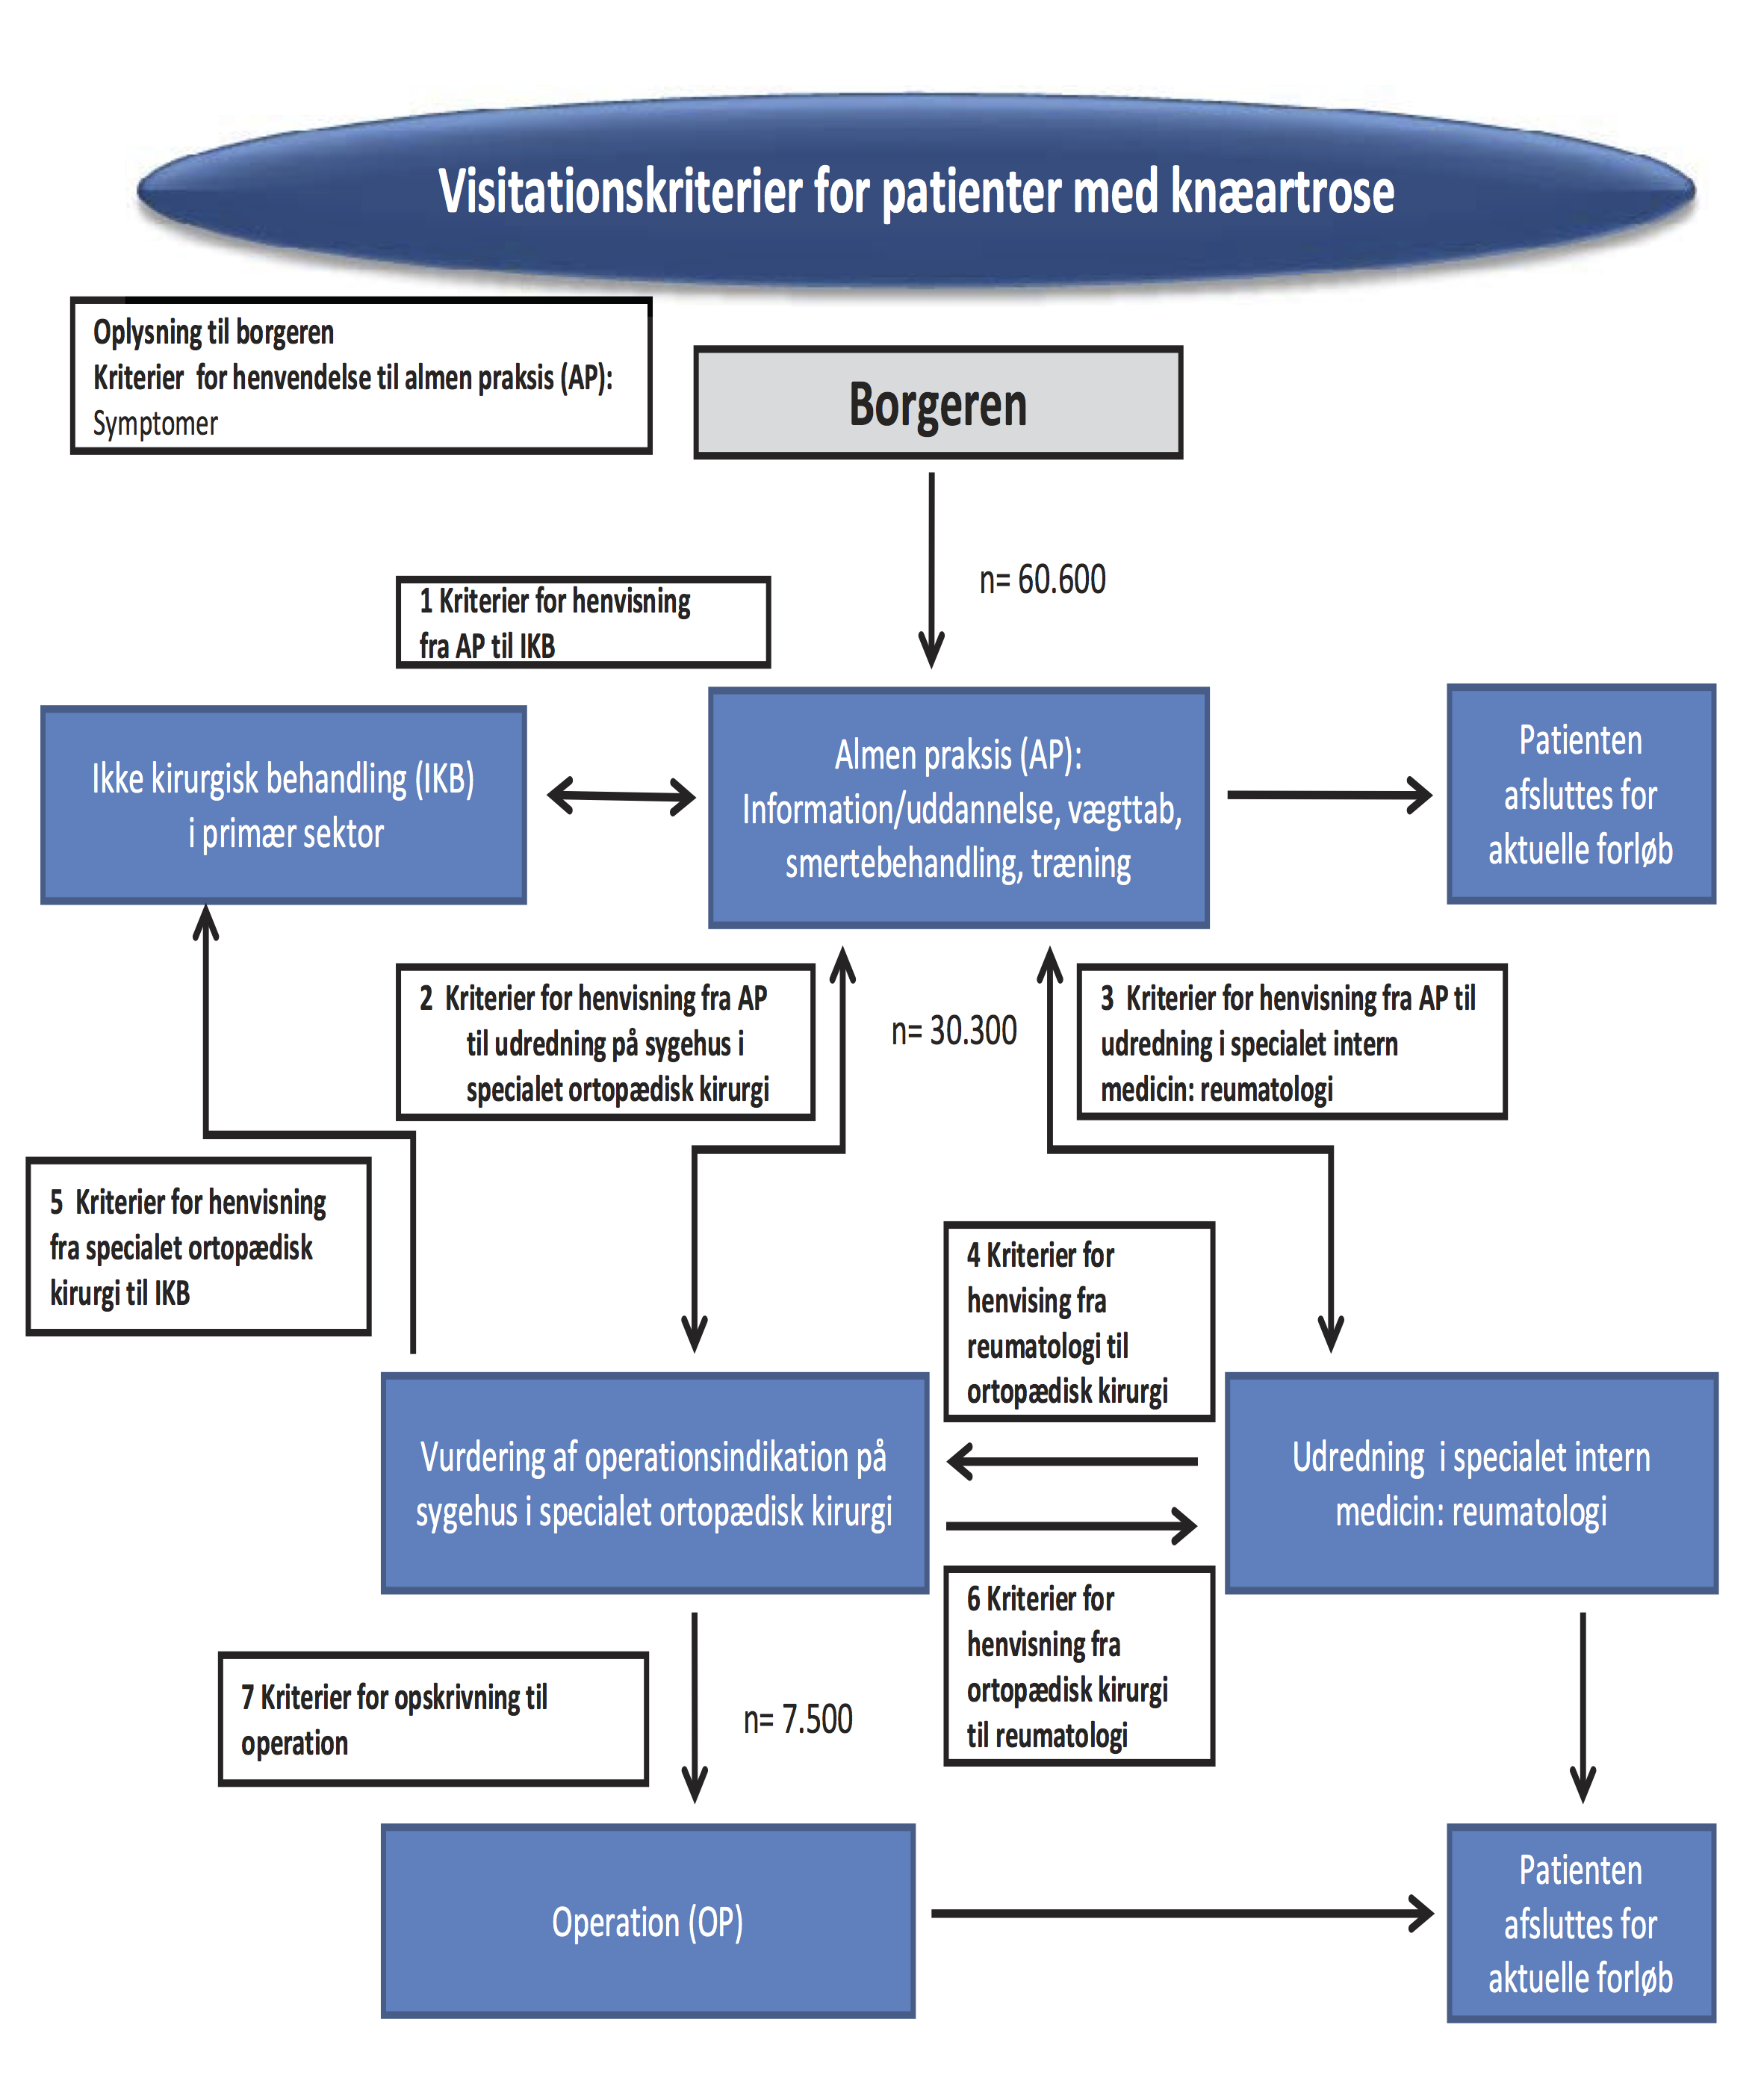
\includegraphics[width=0.9\textwidth]{rapportAfsnit/qBilag/Borgerforloeb}
	\end{center}
	\caption{Flowchartet viser hvordan en patient med knæarterose visiteres. Både i forhold til primær og sekundær sektor. \citep{brostrom2012}}
	\label{} 
\end{figure}
	\chapter{Søgeprotokol} \vspace{-.75cm}
\textit{Følgende appendiks indeholder søgeprotokollen for hvert domæne.}
\section{TEC}\label{TEC_sog}
\begin{center}
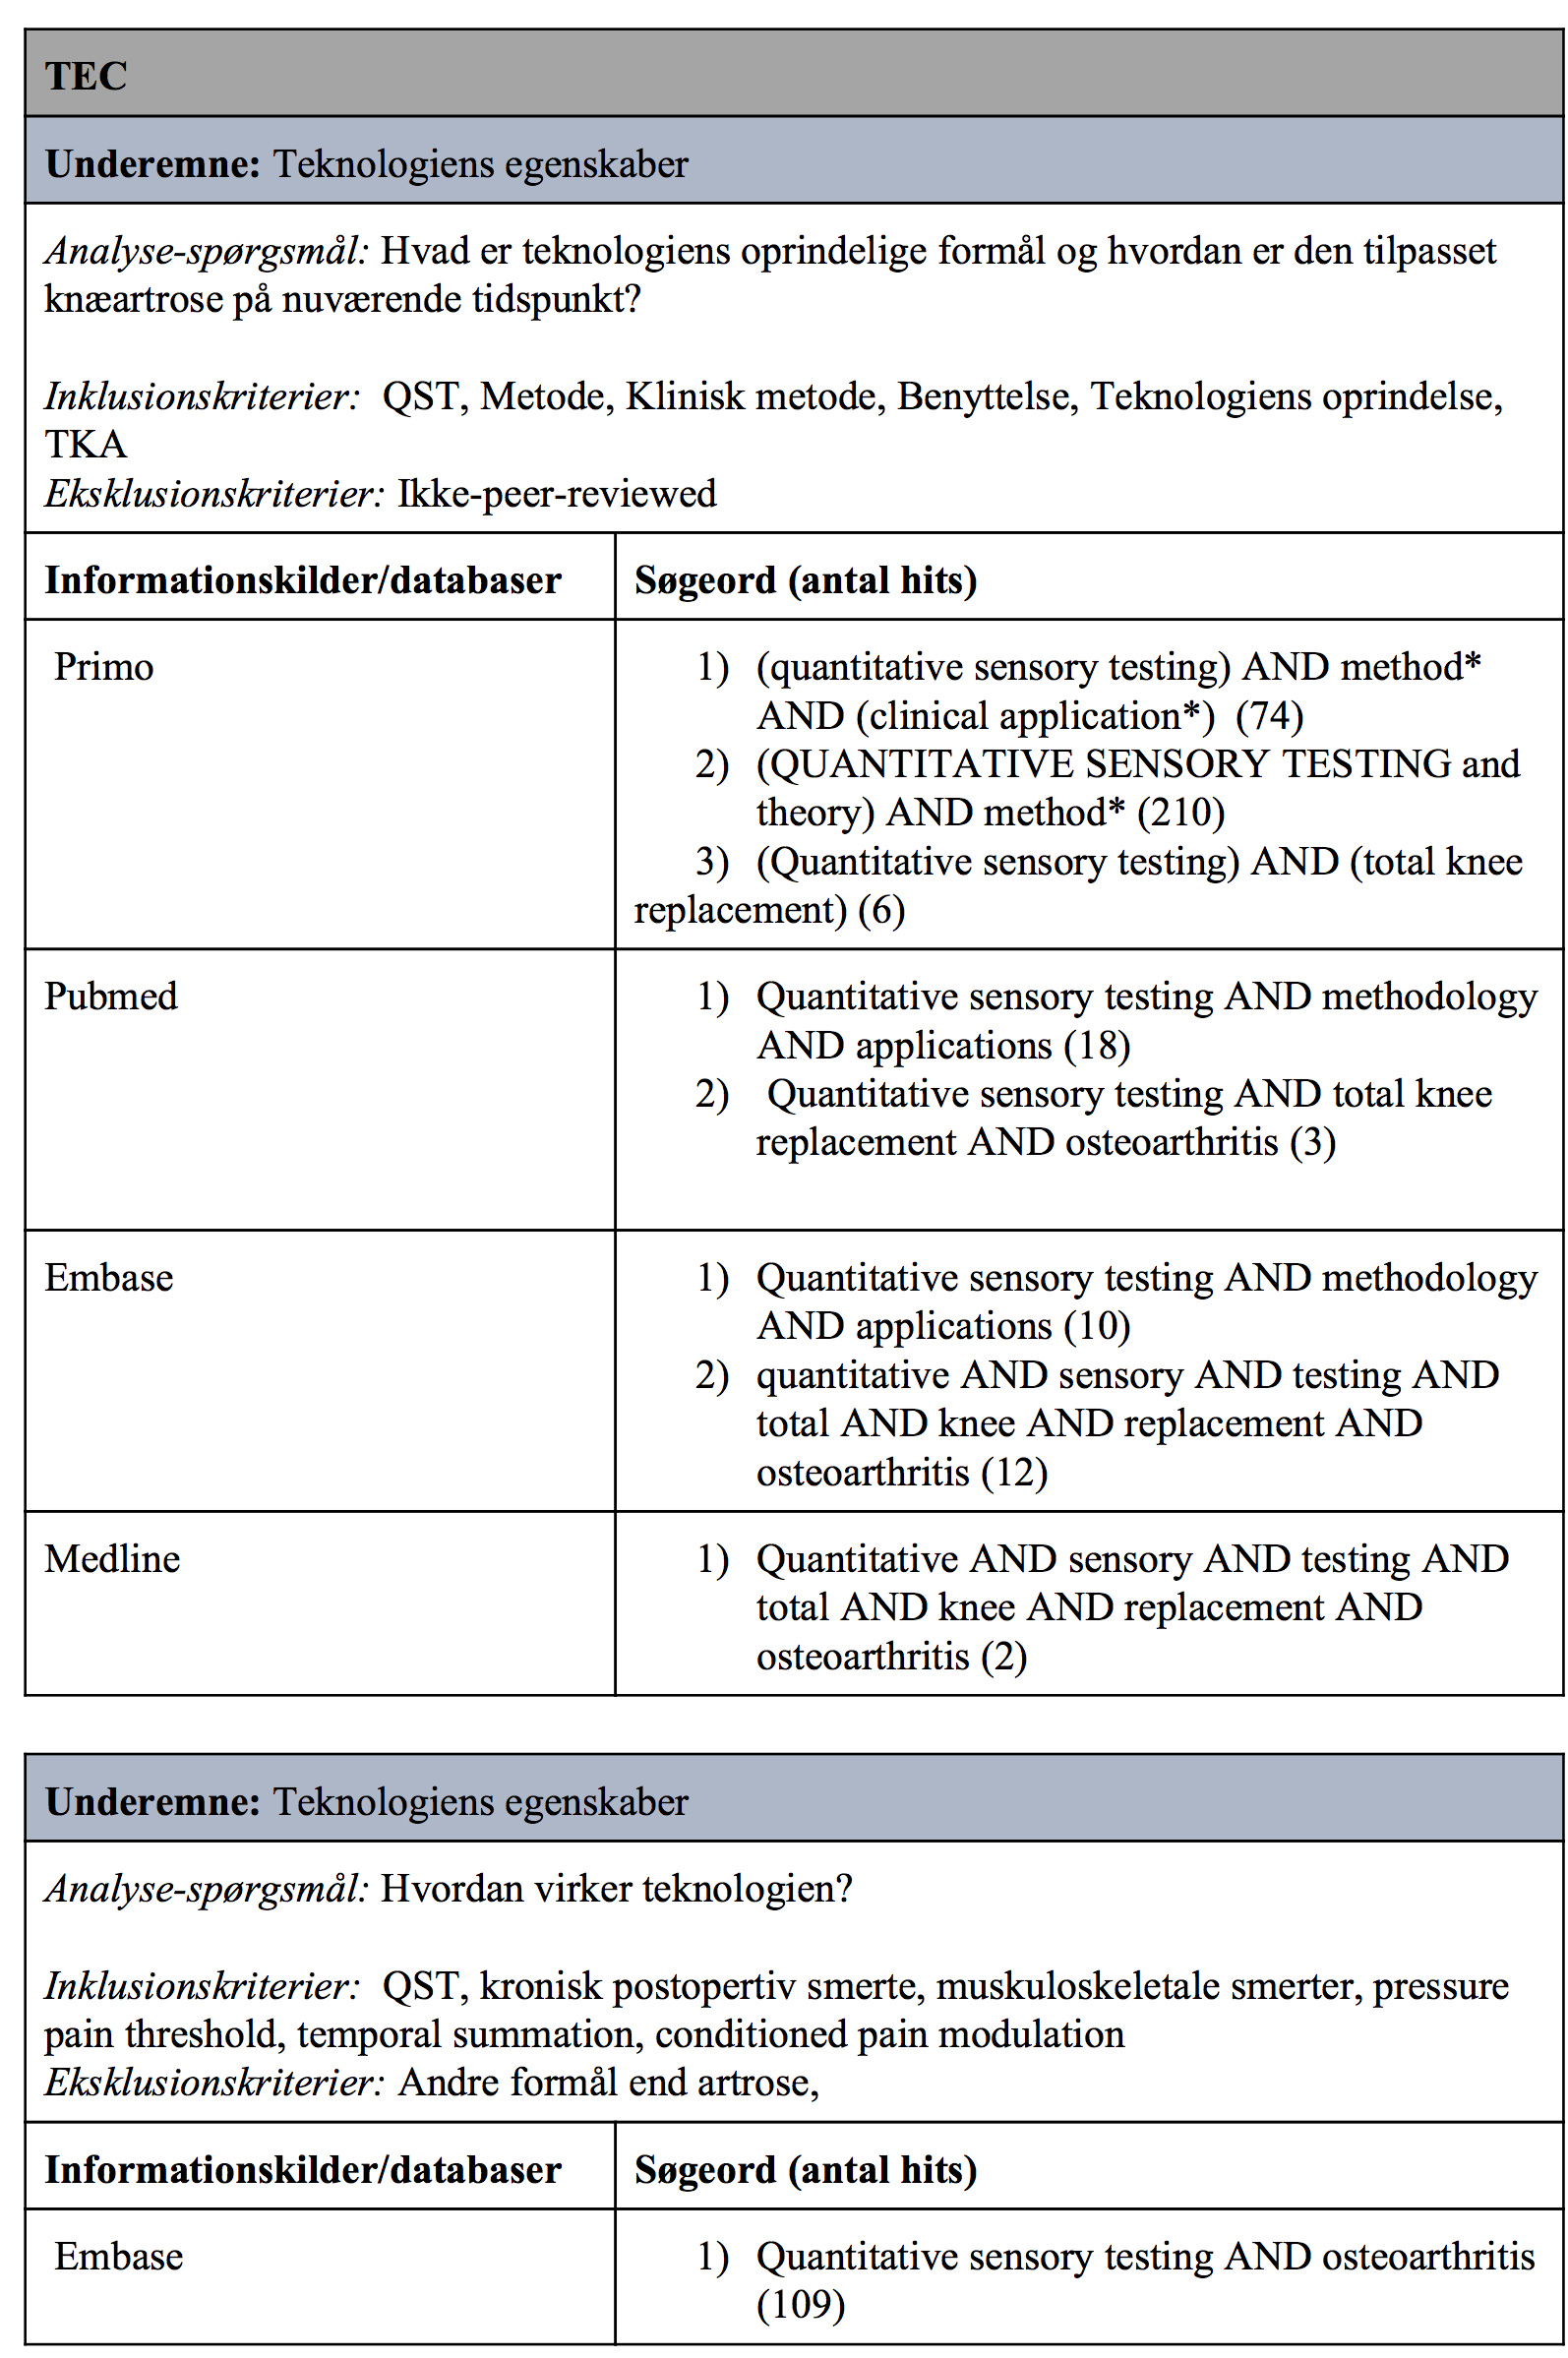
\includegraphics[width=0.8\textwidth]{rapportAfsnit/qBilag/sogninger/TEC1}

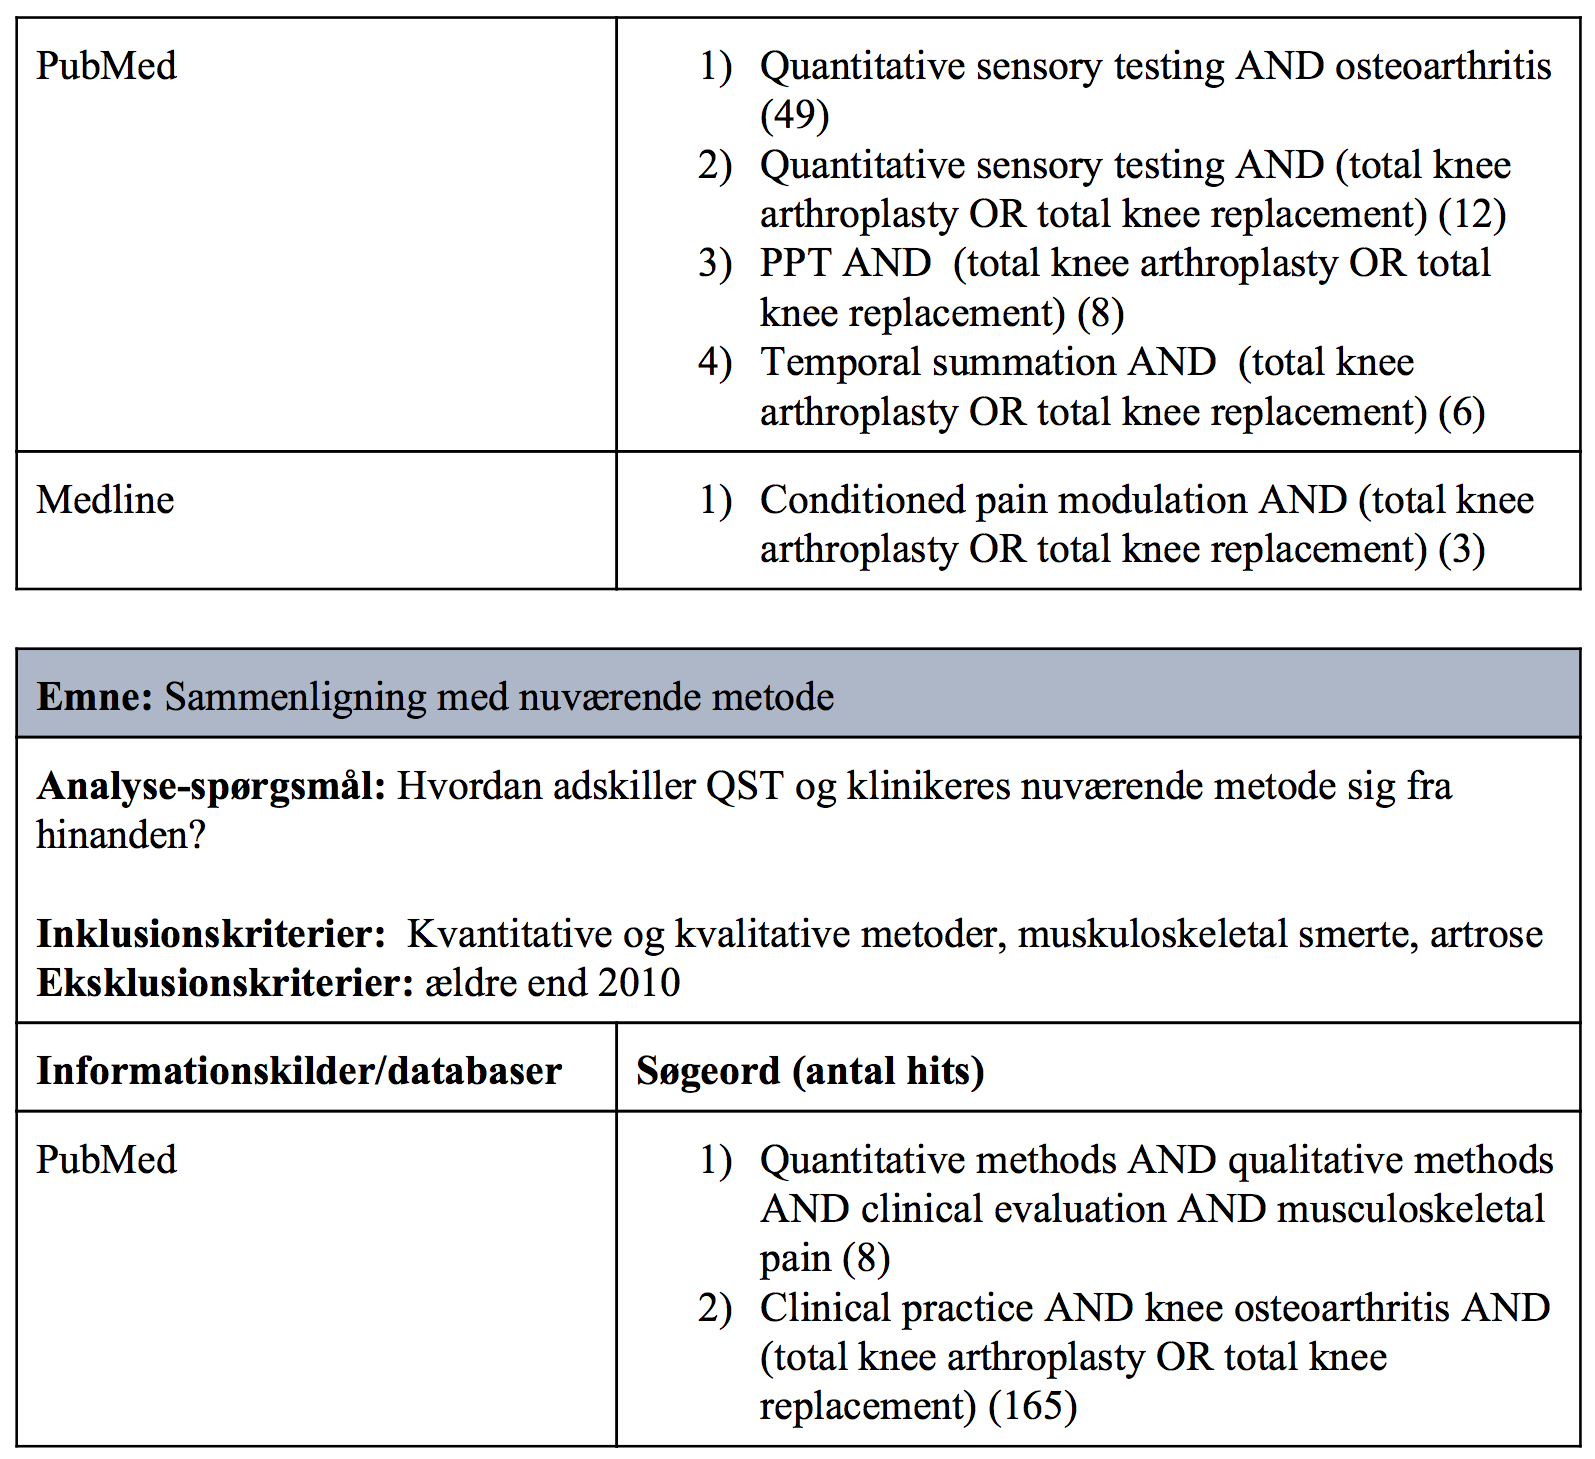
\includegraphics[width=0.8\textwidth]{rapportAfsnit/qBilag/sogninger/TEC2}
\end{center}

\section{EFF}\label{EFF_sog}
\begin{center}
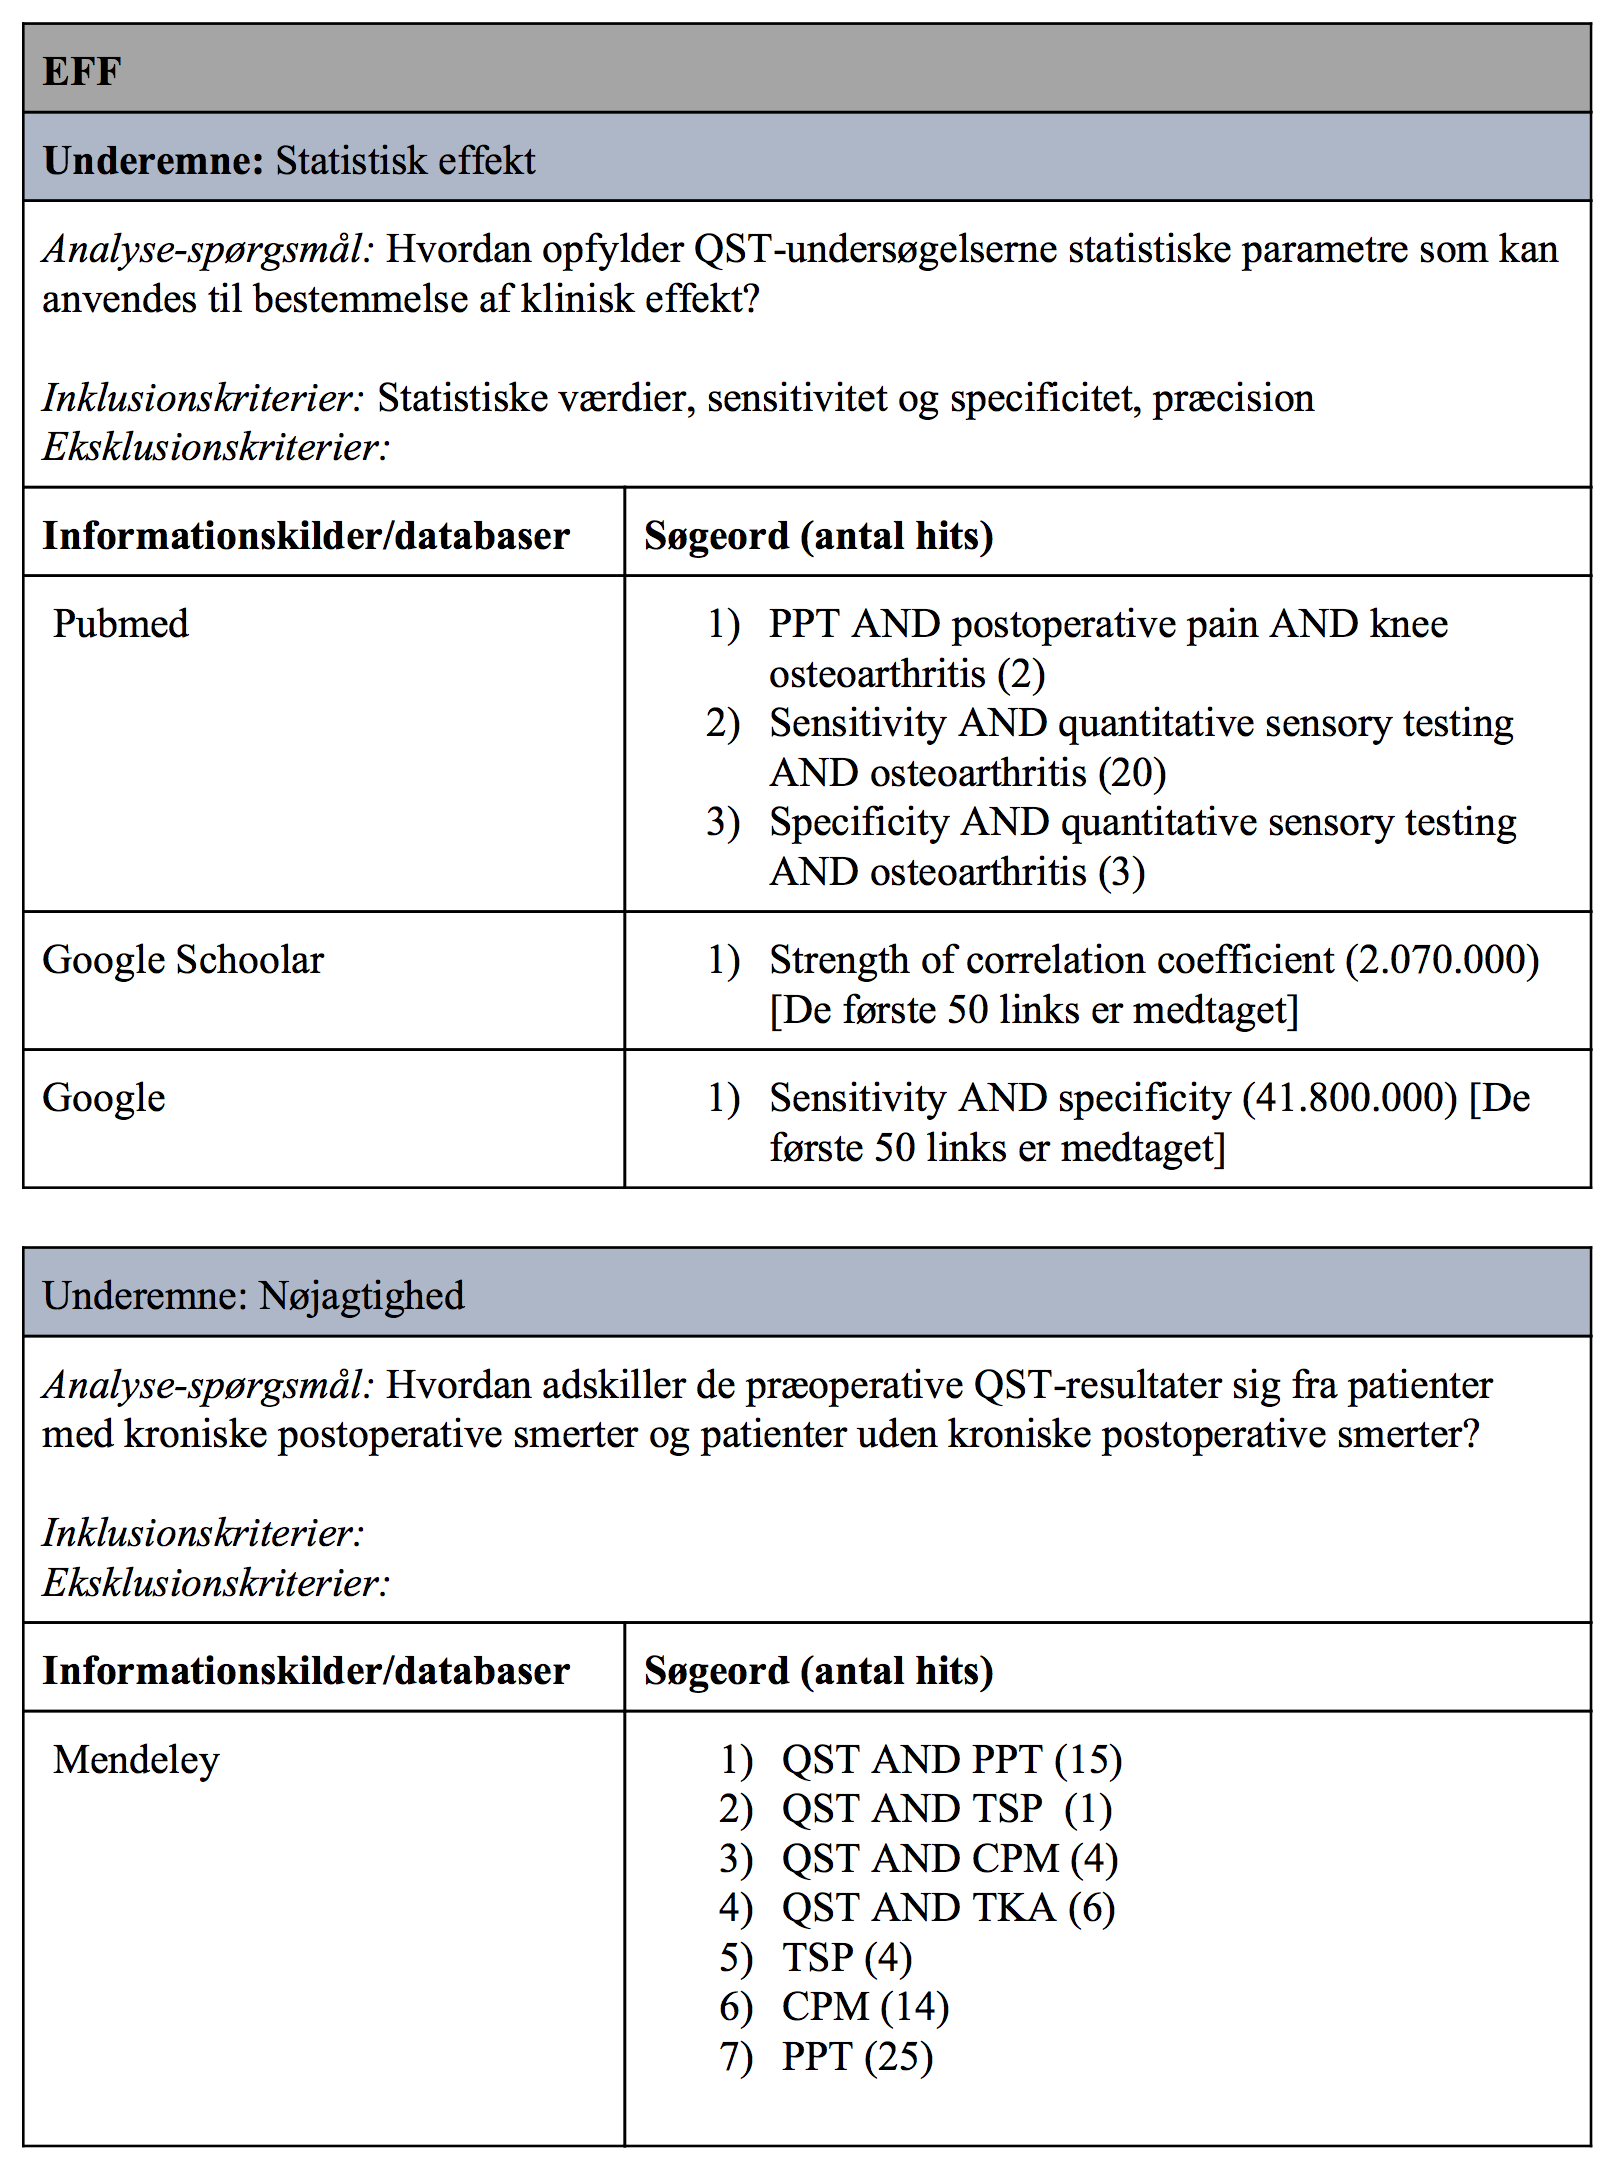
\includegraphics[width=0.8\textwidth]{rapportAfsnit/qBilag/sogninger/EFF1}

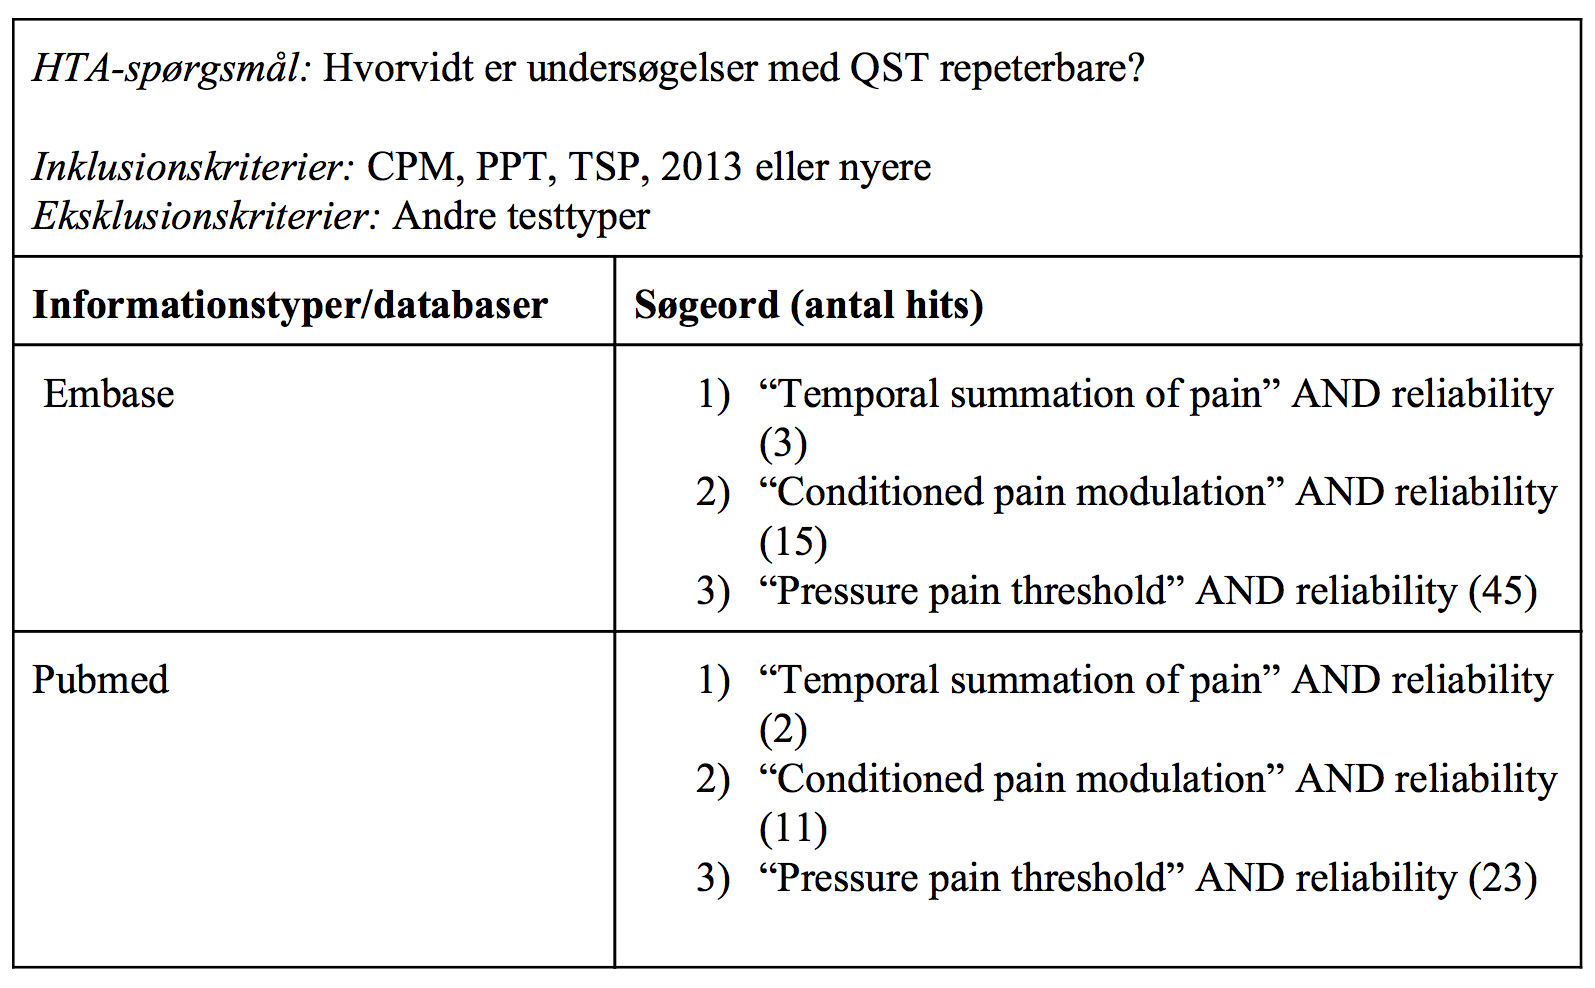
\includegraphics[width=0.8\textwidth]{rapportAfsnit/qBilag/sogninger/EFF2}
\end{center}

\section{ECO}\label{ECO_sog}
\begin{center}
	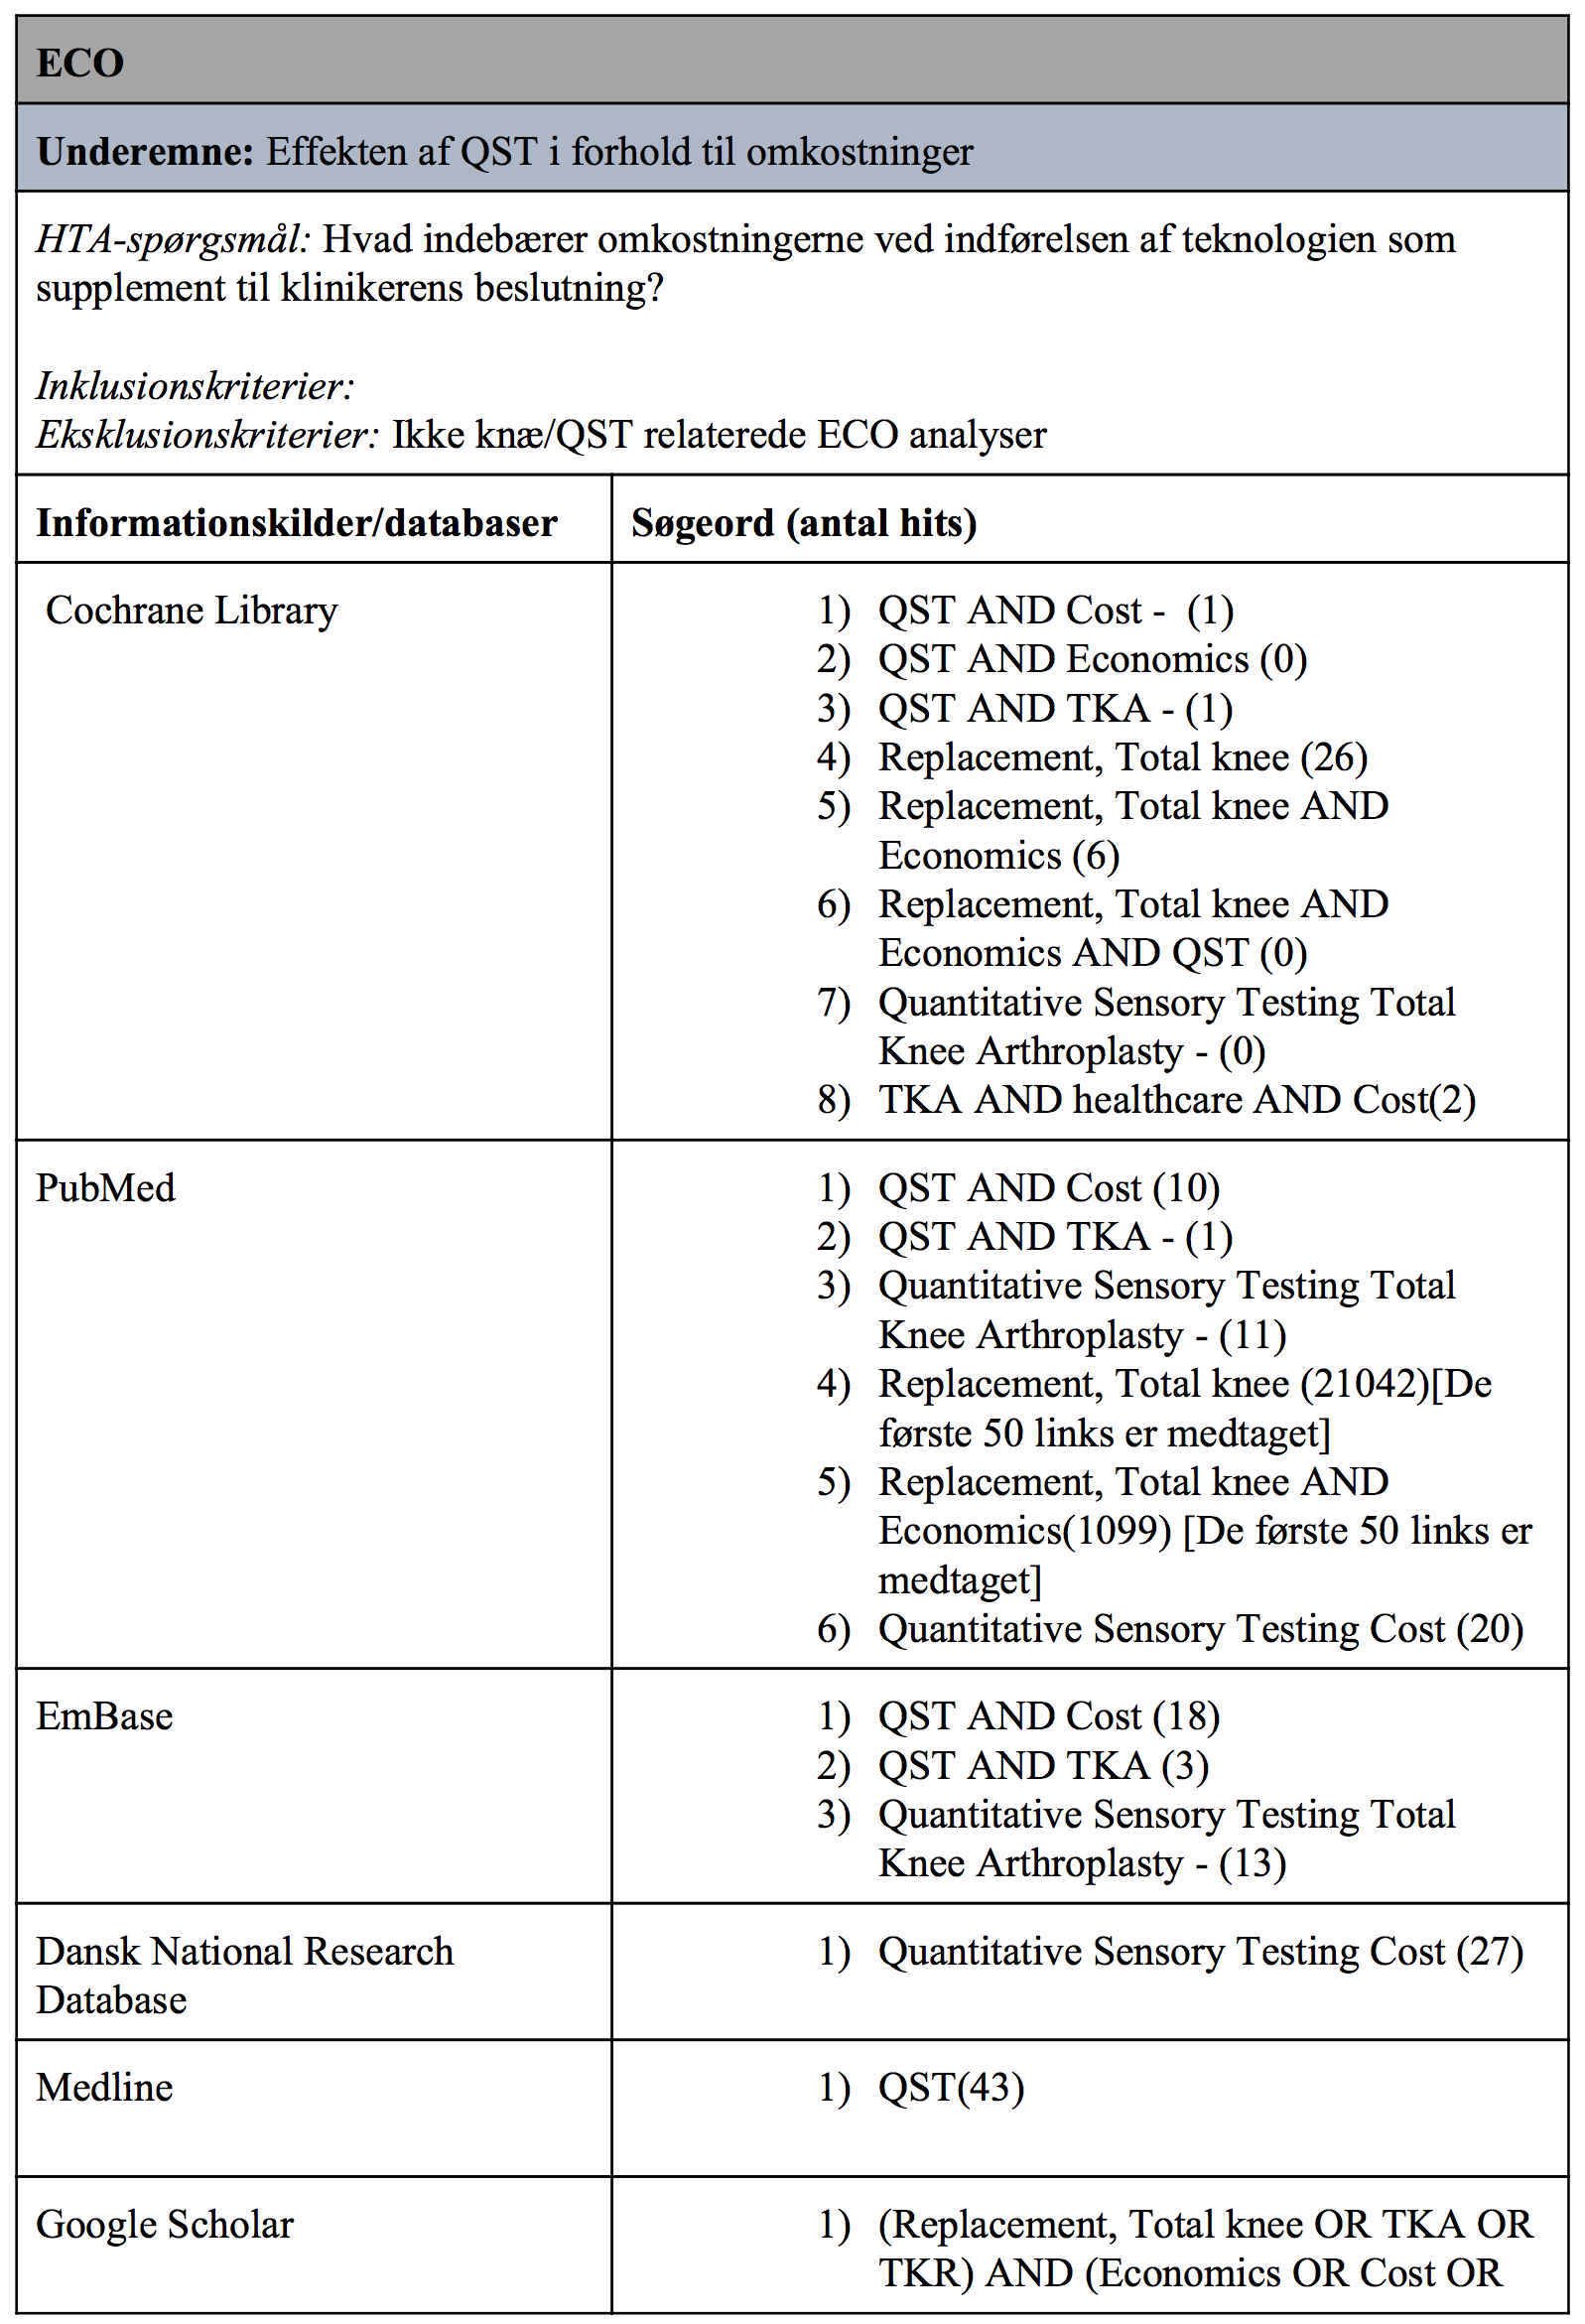
\includegraphics[width=0.8\textwidth]{rapportAfsnit/qBilag/sogninger/ECO1}
	
	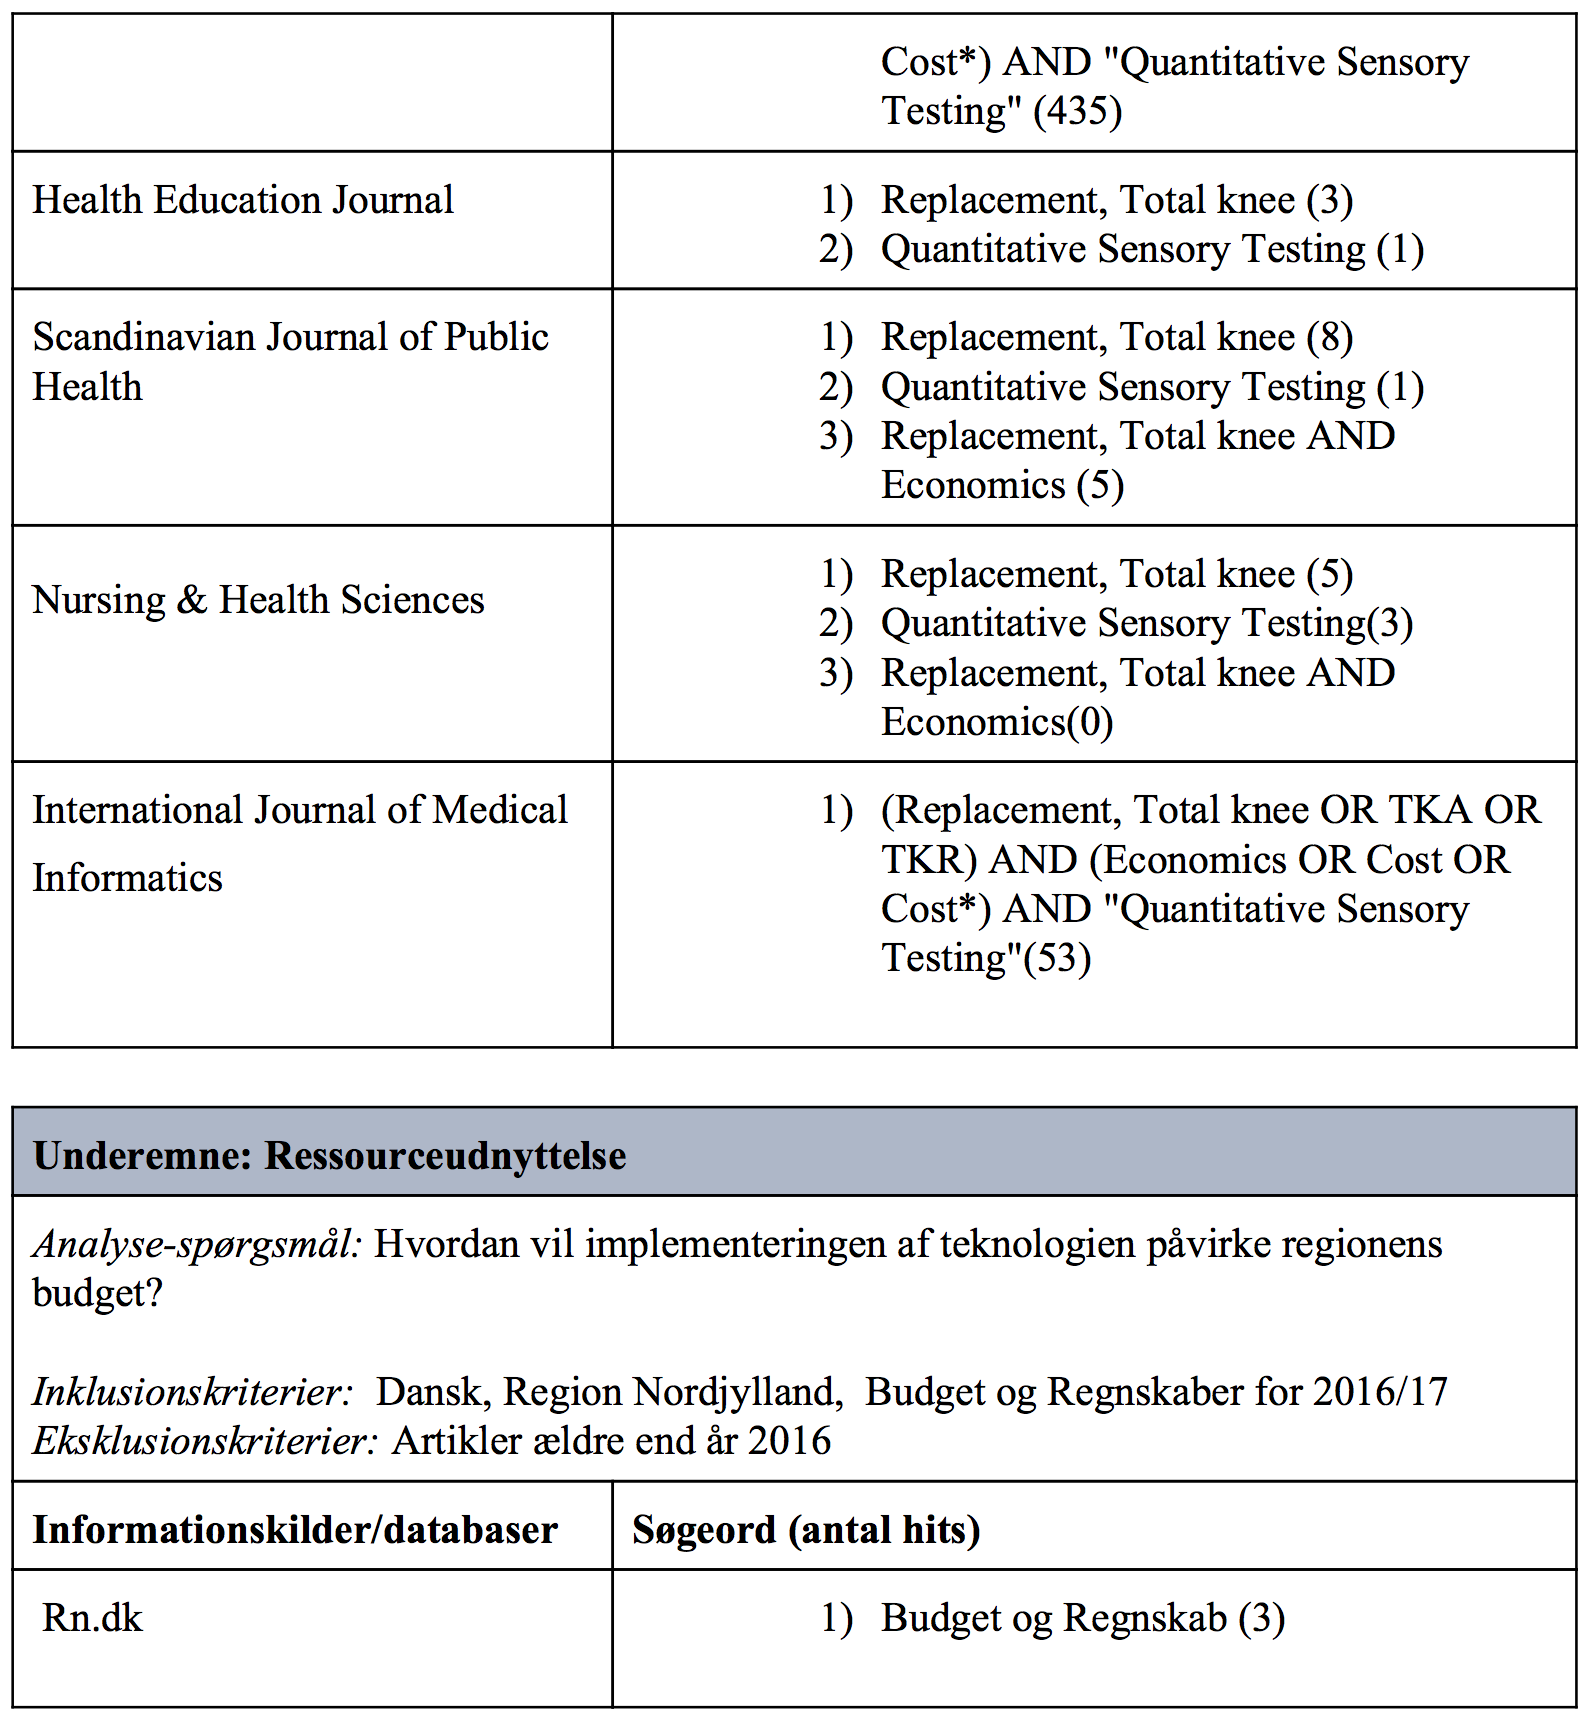
\includegraphics[width=0.8\textwidth]{rapportAfsnit/qBilag/sogninger/ECO2}
\end{center}

\section{ORG}\label{ORG_sog}
\begin{center}
	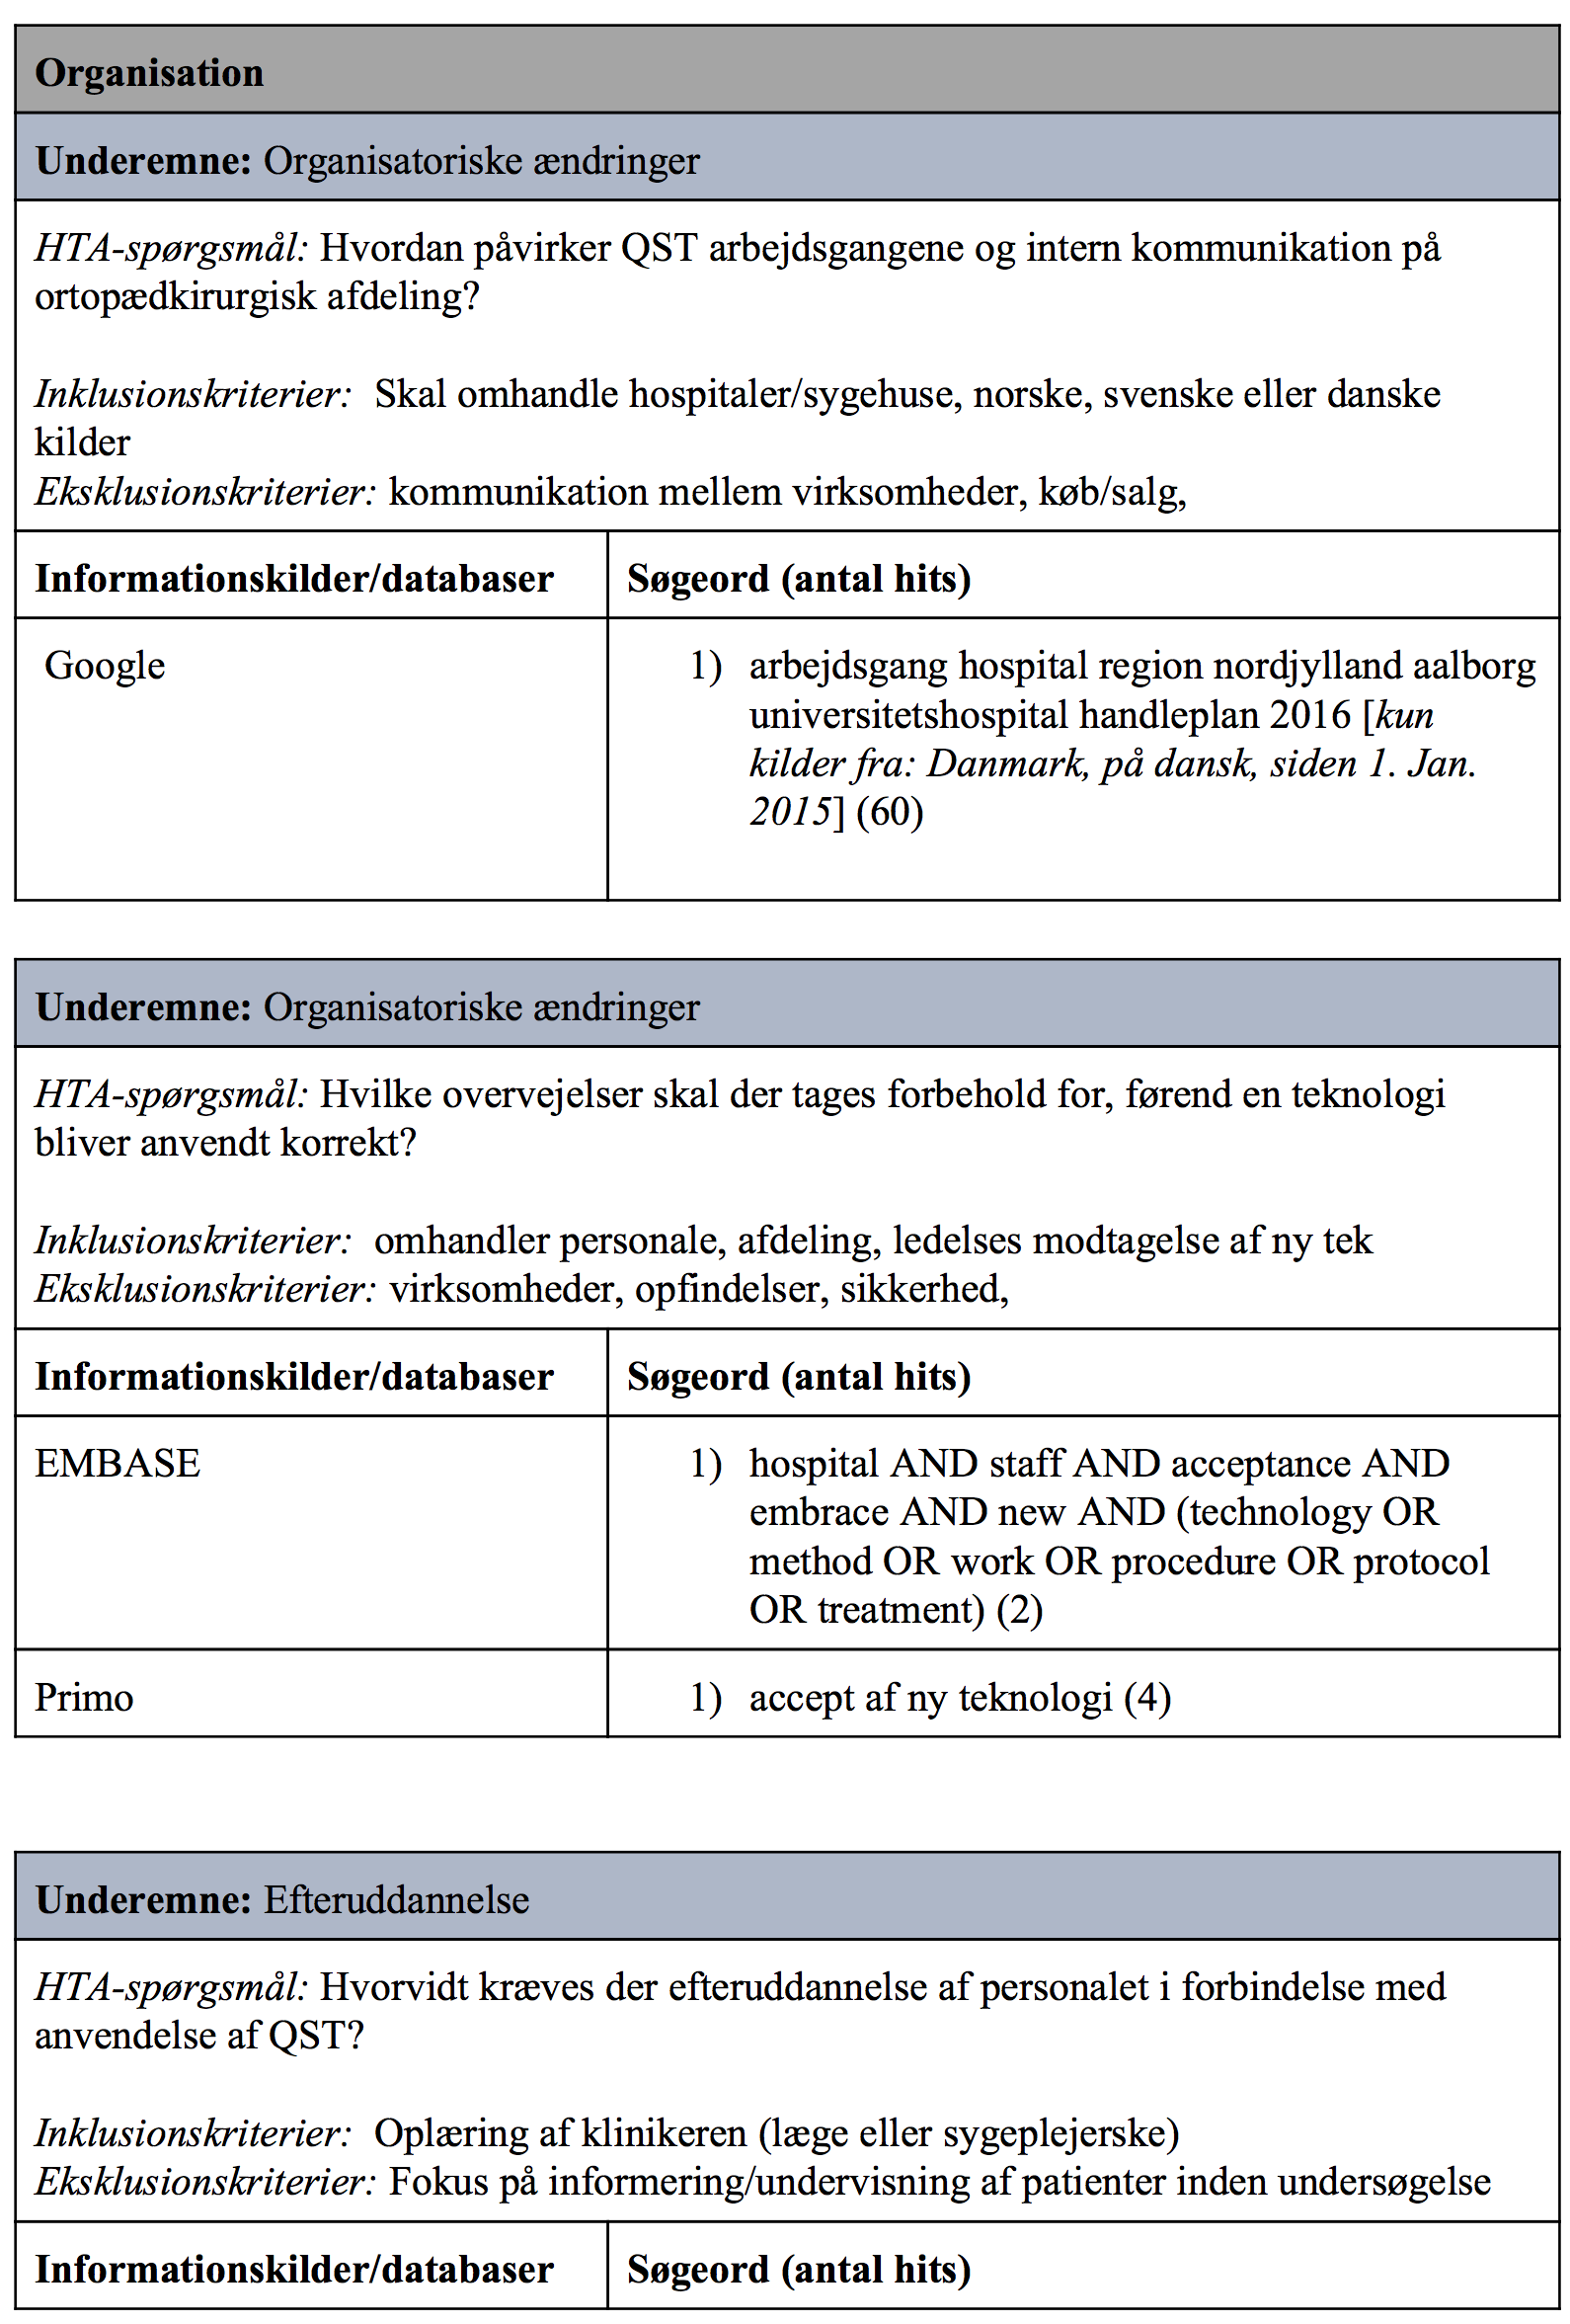
\includegraphics[width=0.8\textwidth]{rapportAfsnit/qBilag/sogninger/ORG1}
	
	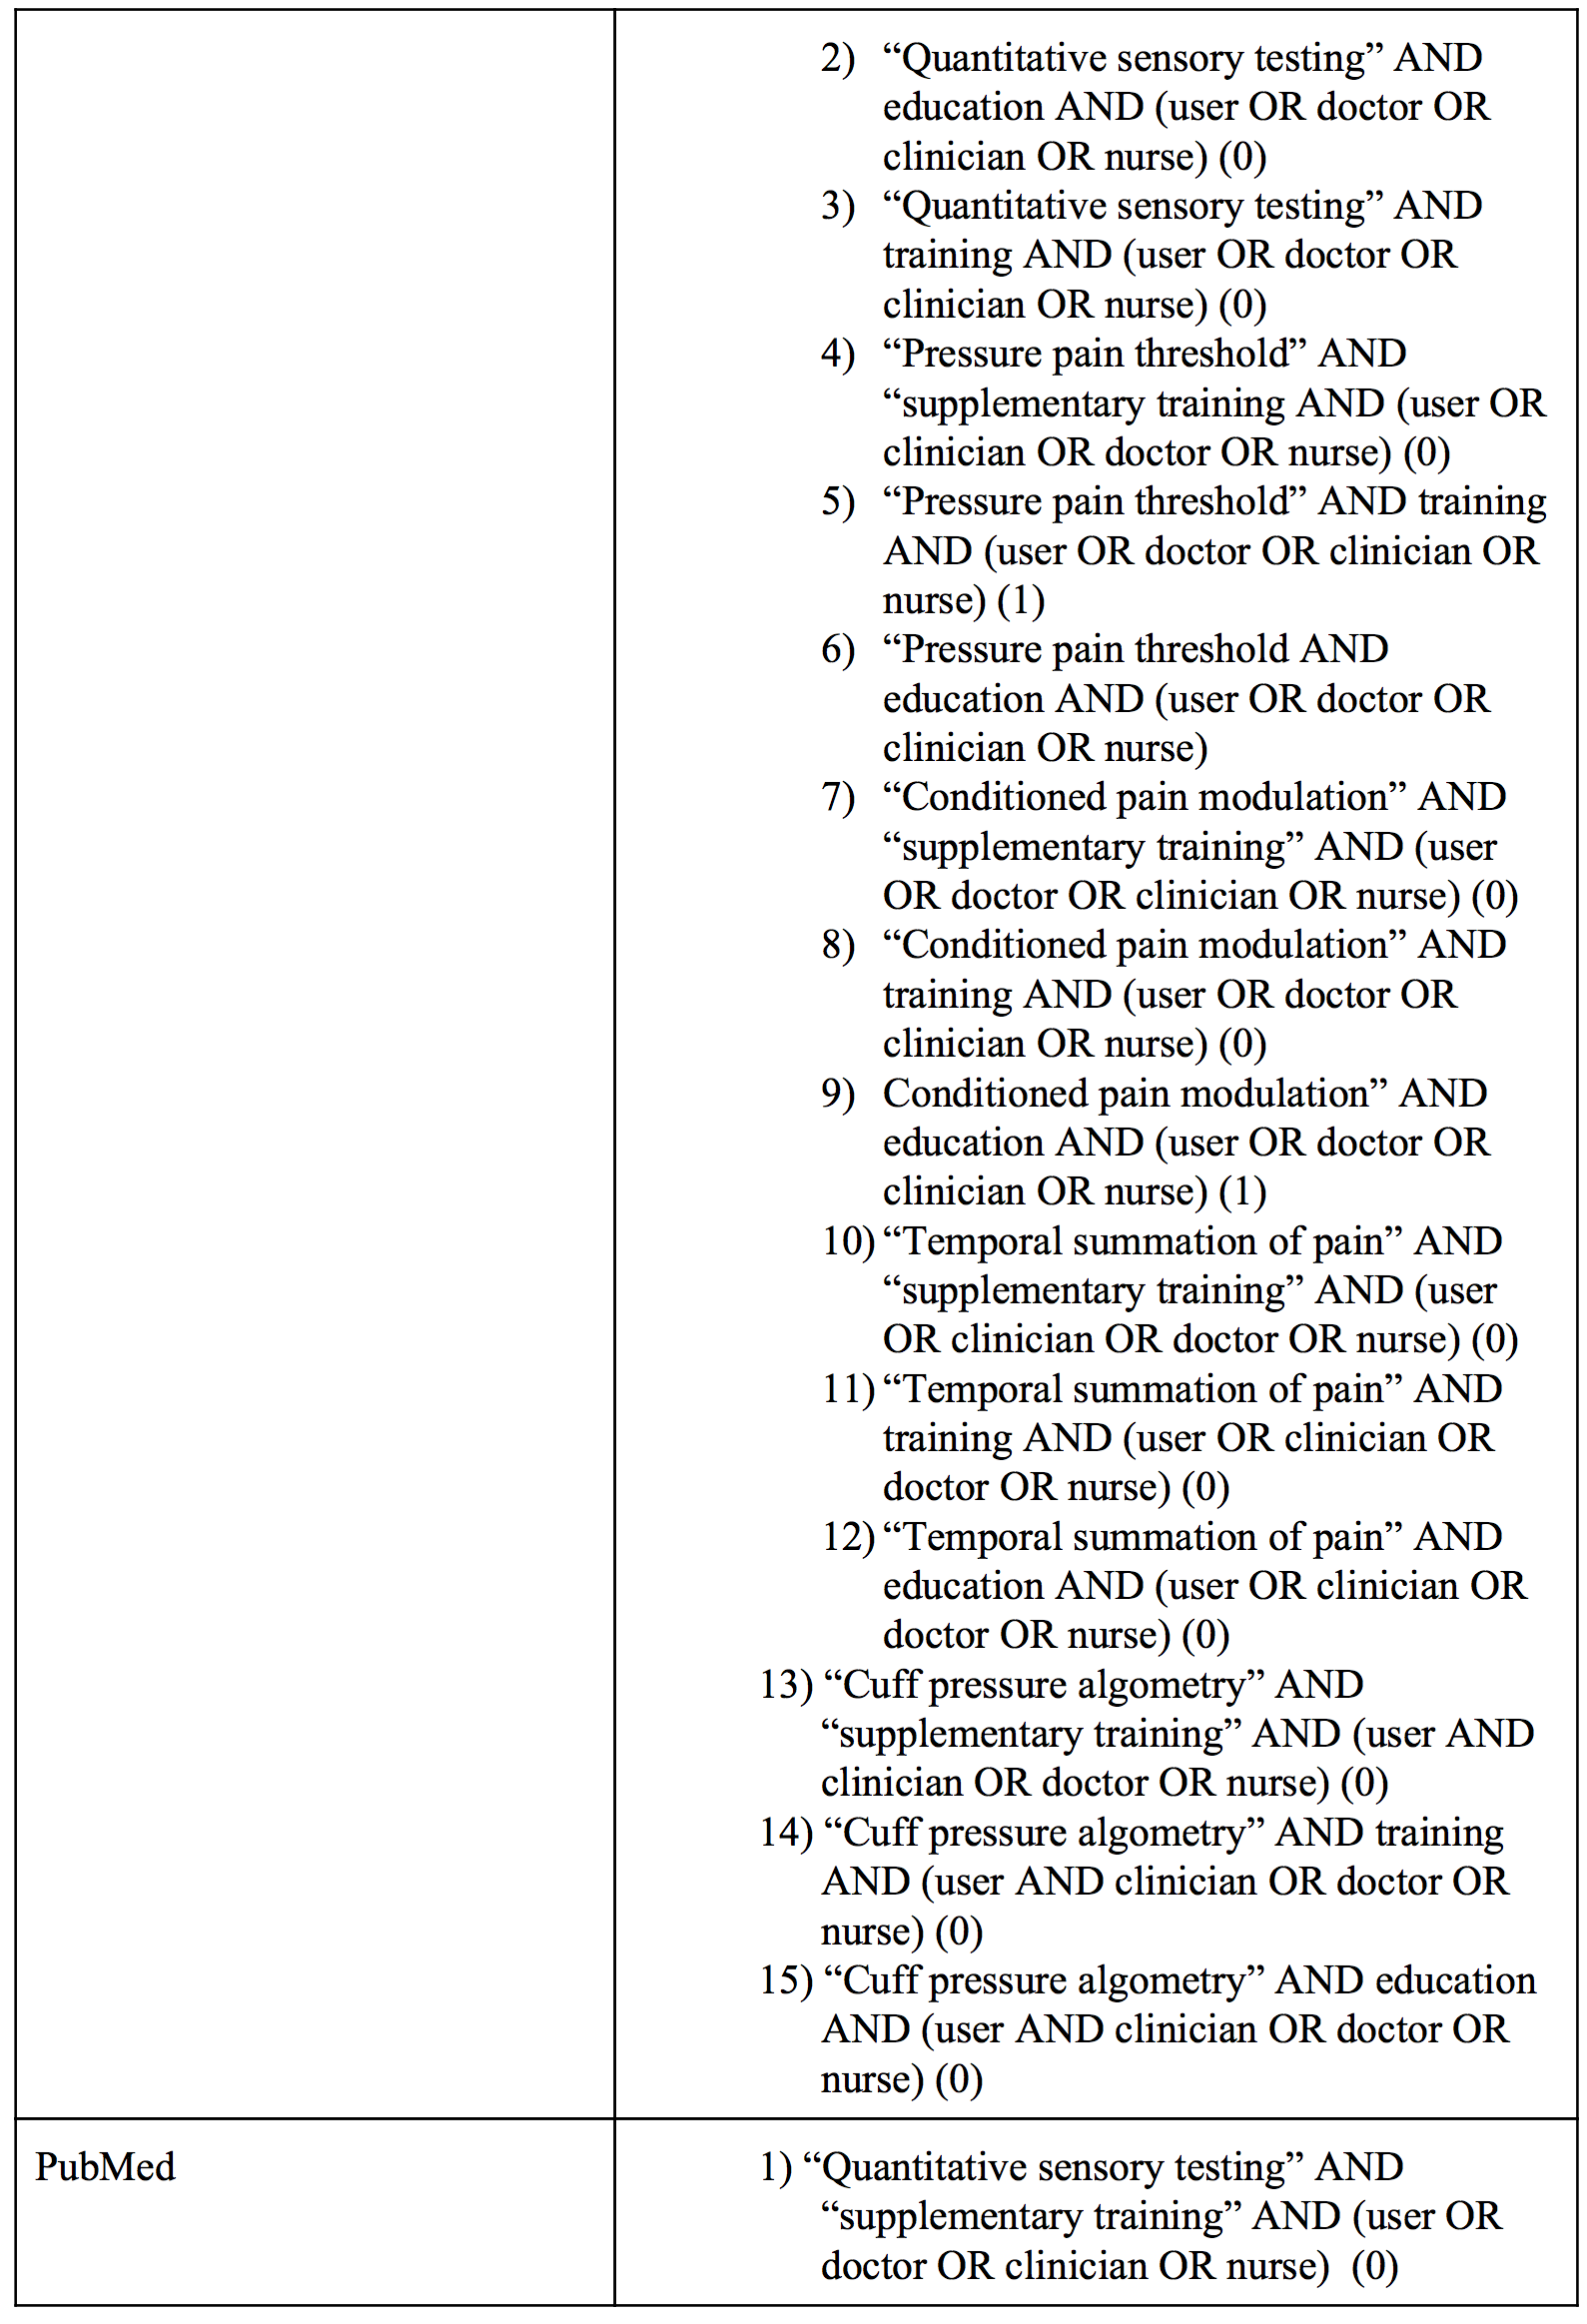
\includegraphics[width=0.8\textwidth]{rapportAfsnit/qBilag/sogninger/ORG2}
	
	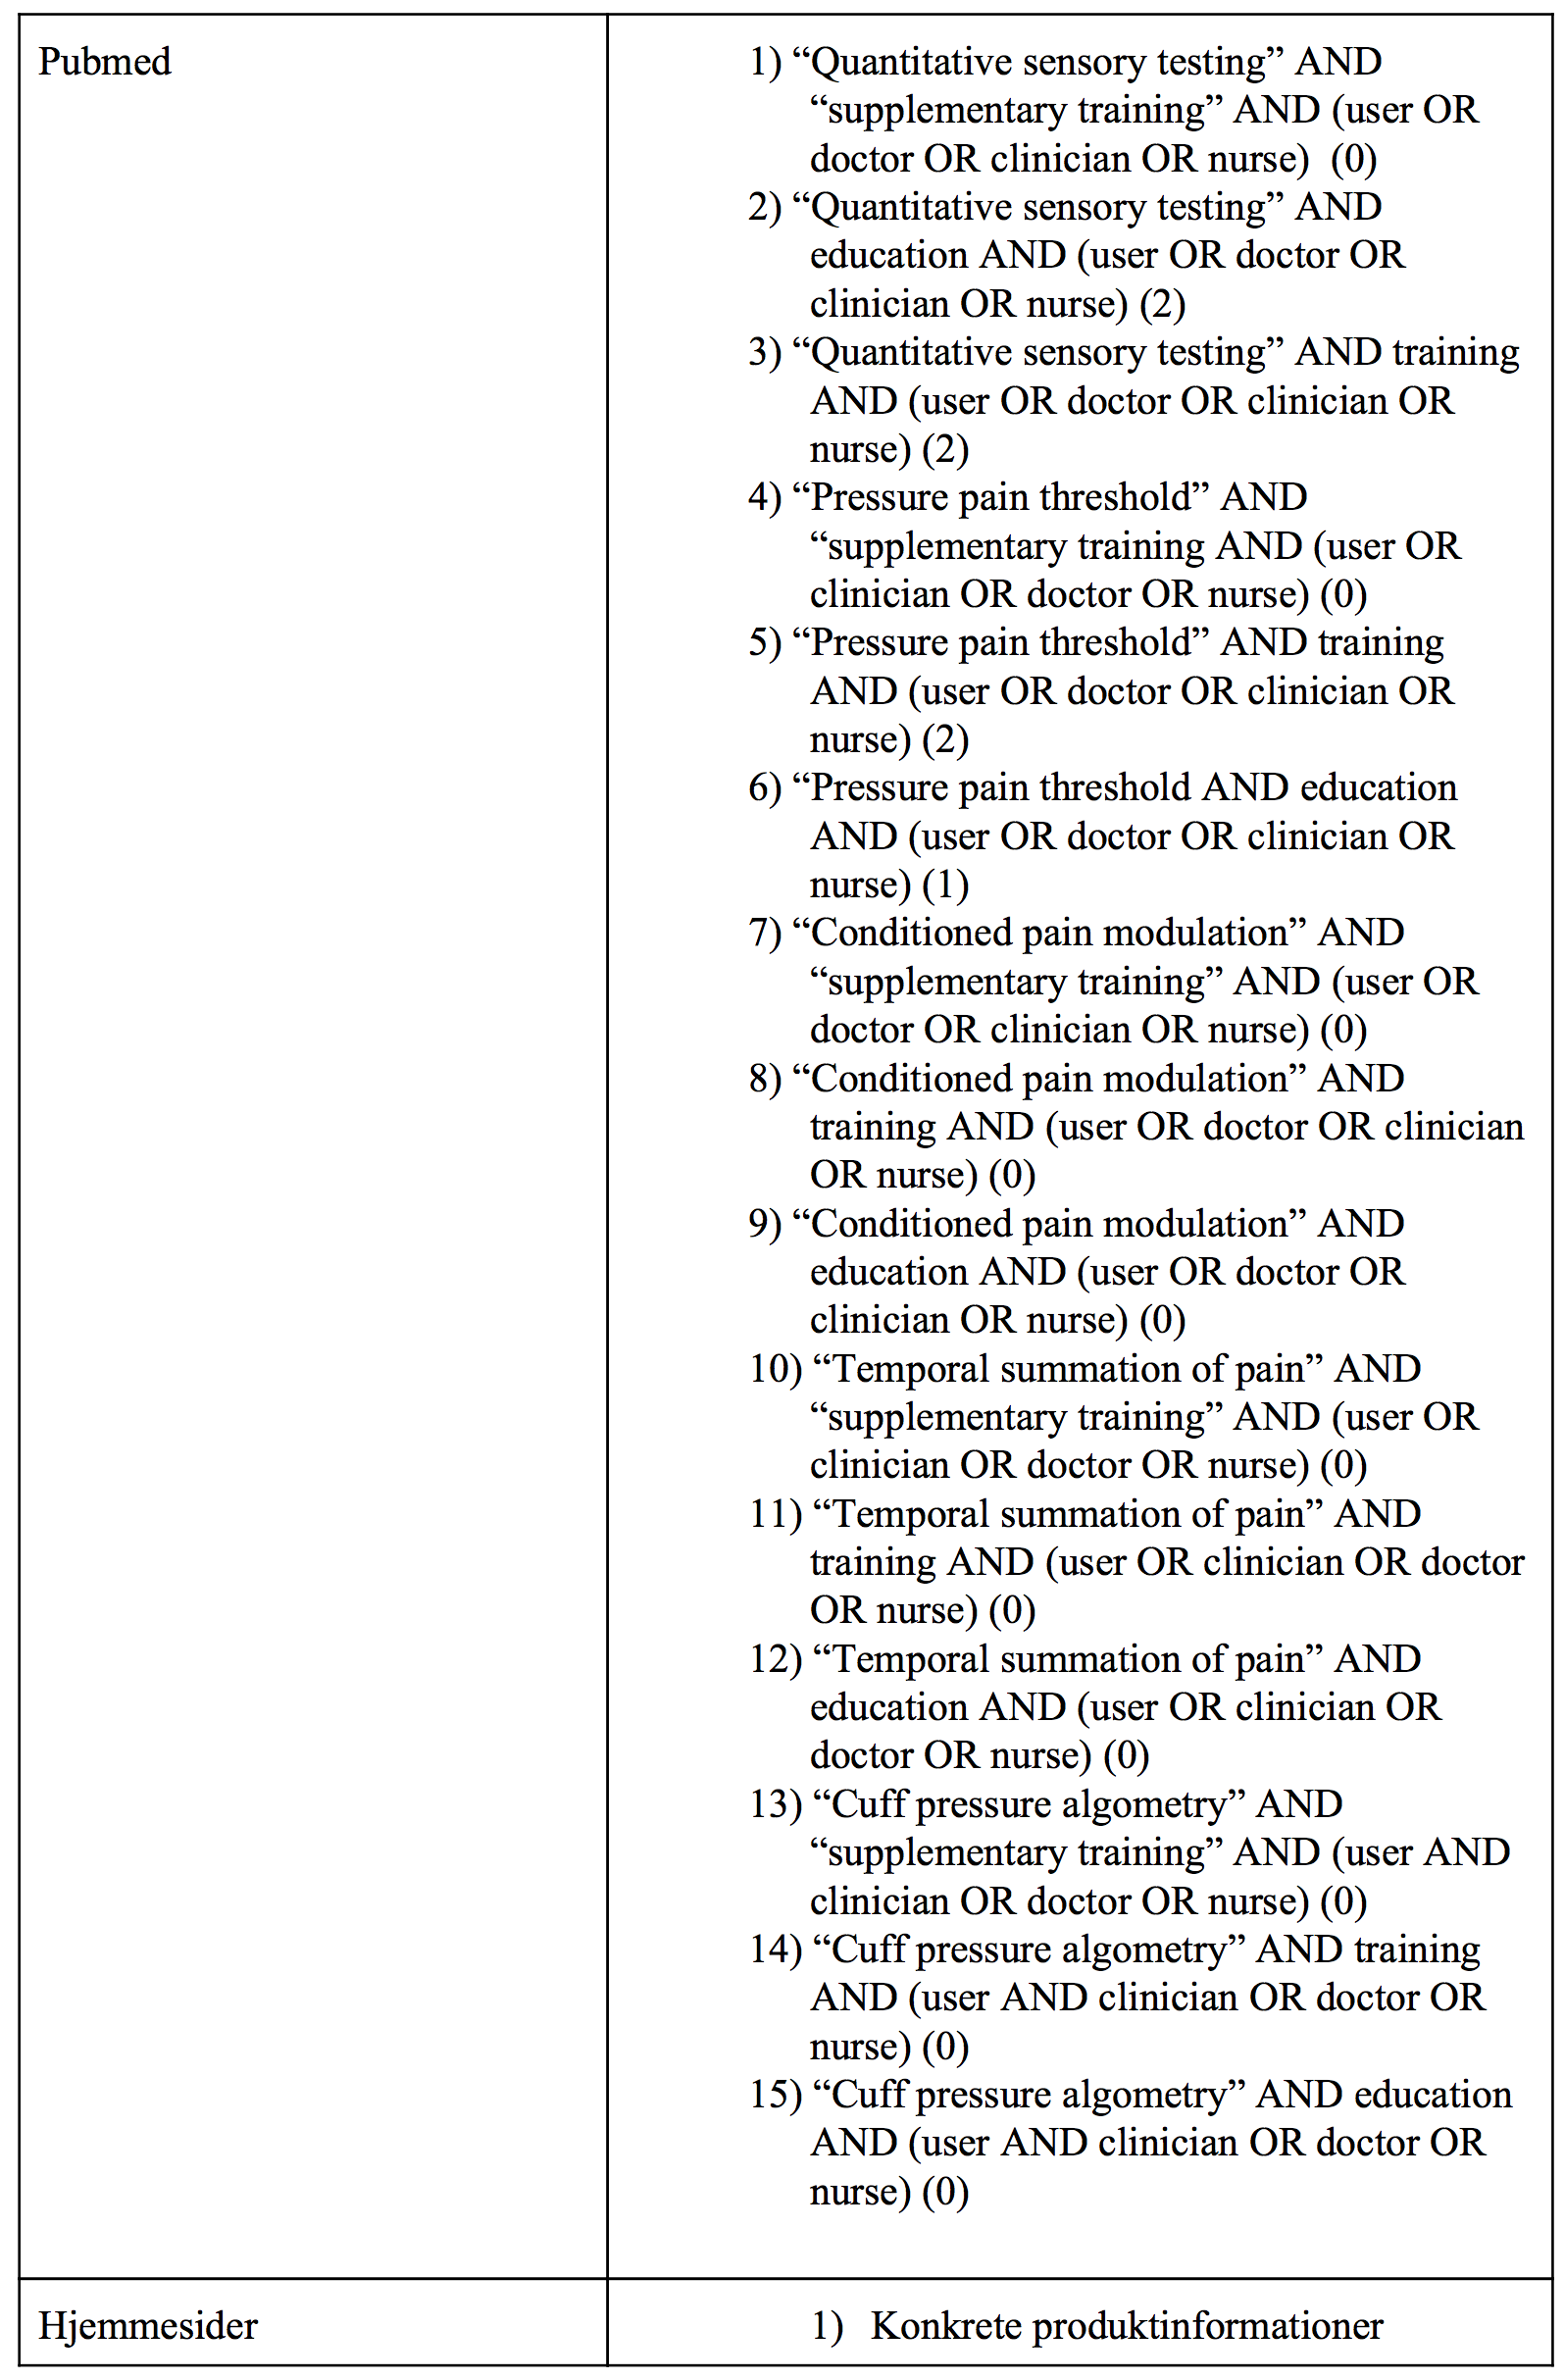
\includegraphics[width=0.8\textwidth]{rapportAfsnit/qBilag/sogninger/ORG3}
	
	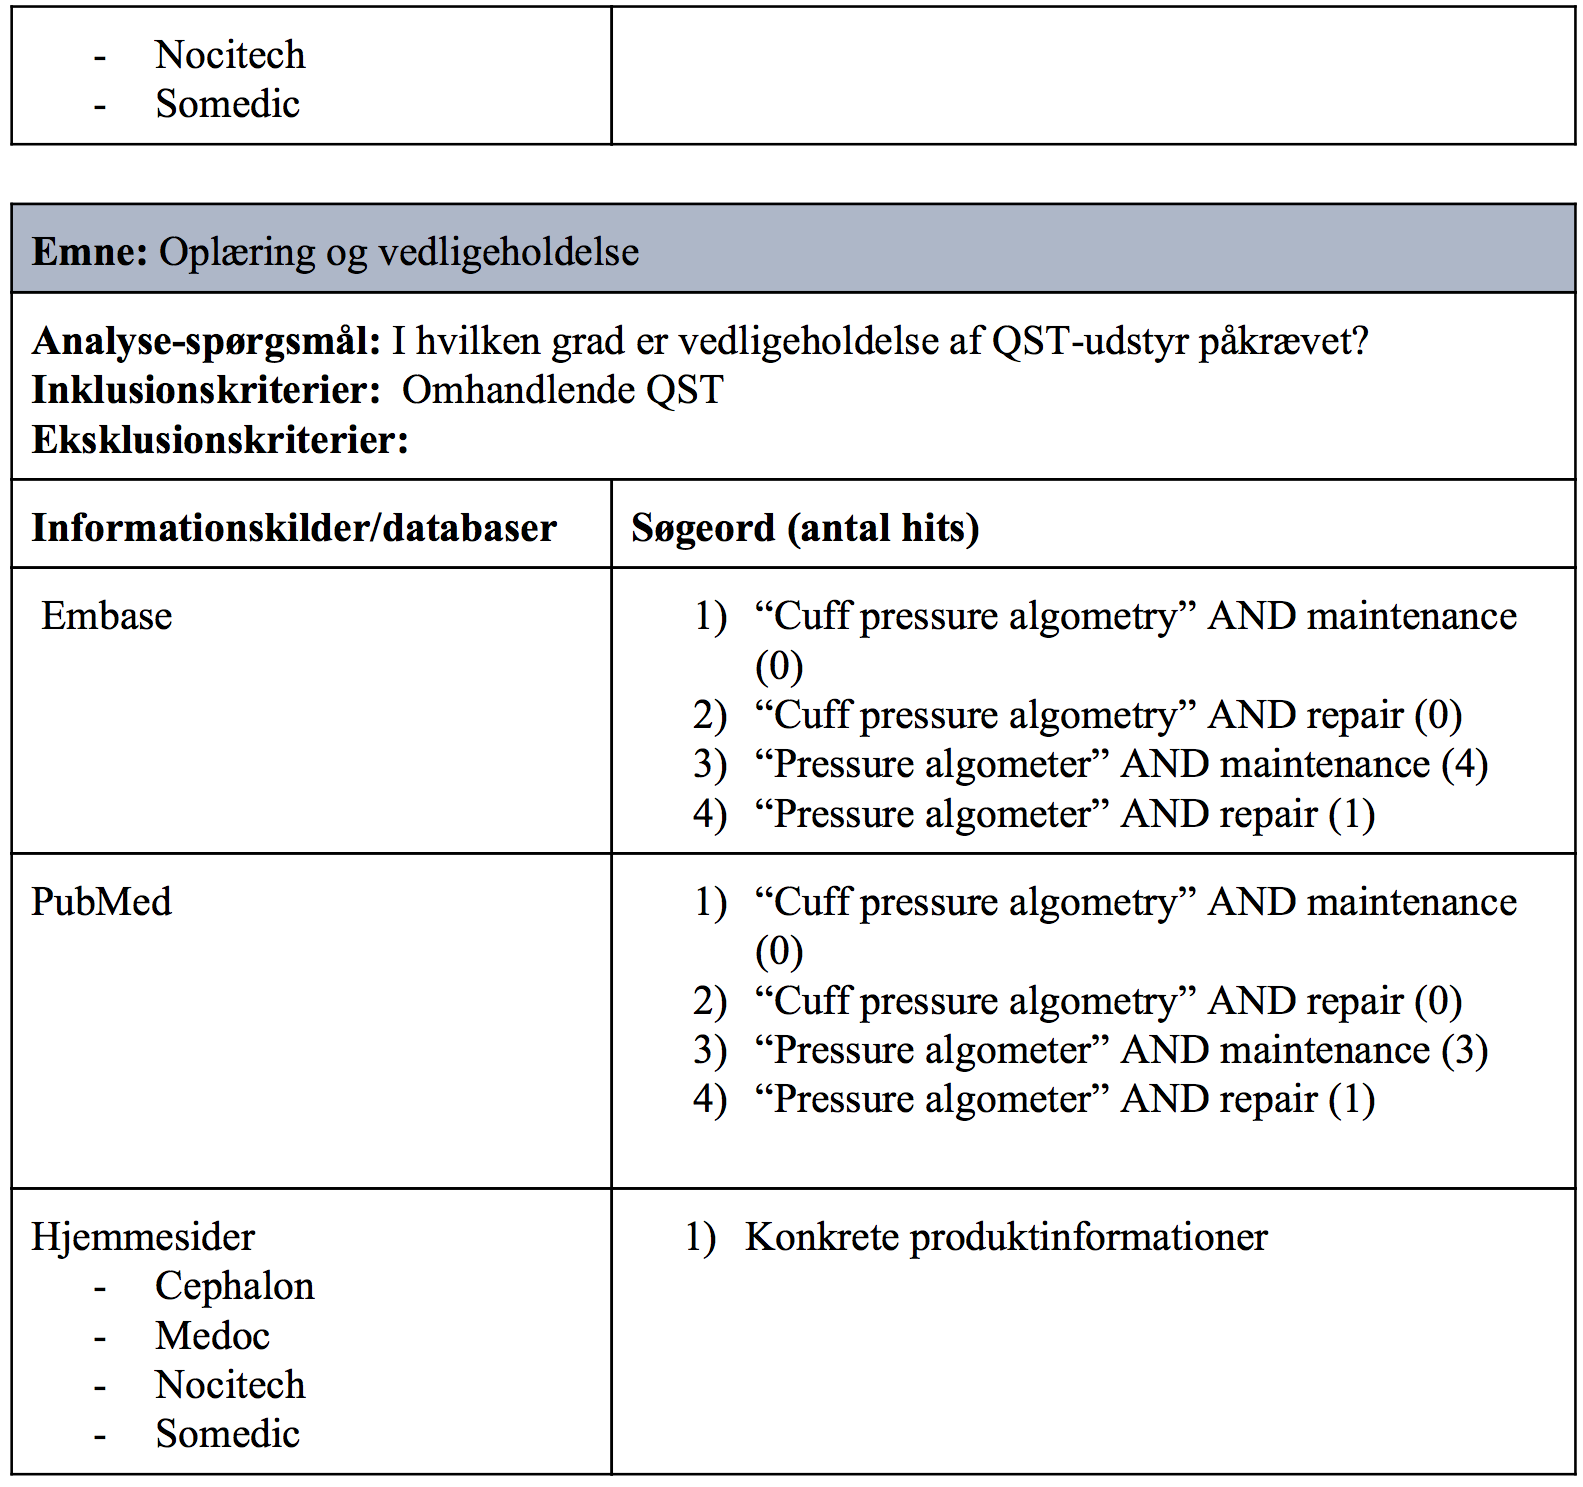
\includegraphics[width=0.8\textwidth]{rapportAfsnit/qBilag/sogninger/ORG4}
\end{center}

\section{SAF}\label{SAF_sog}
\begin{center}
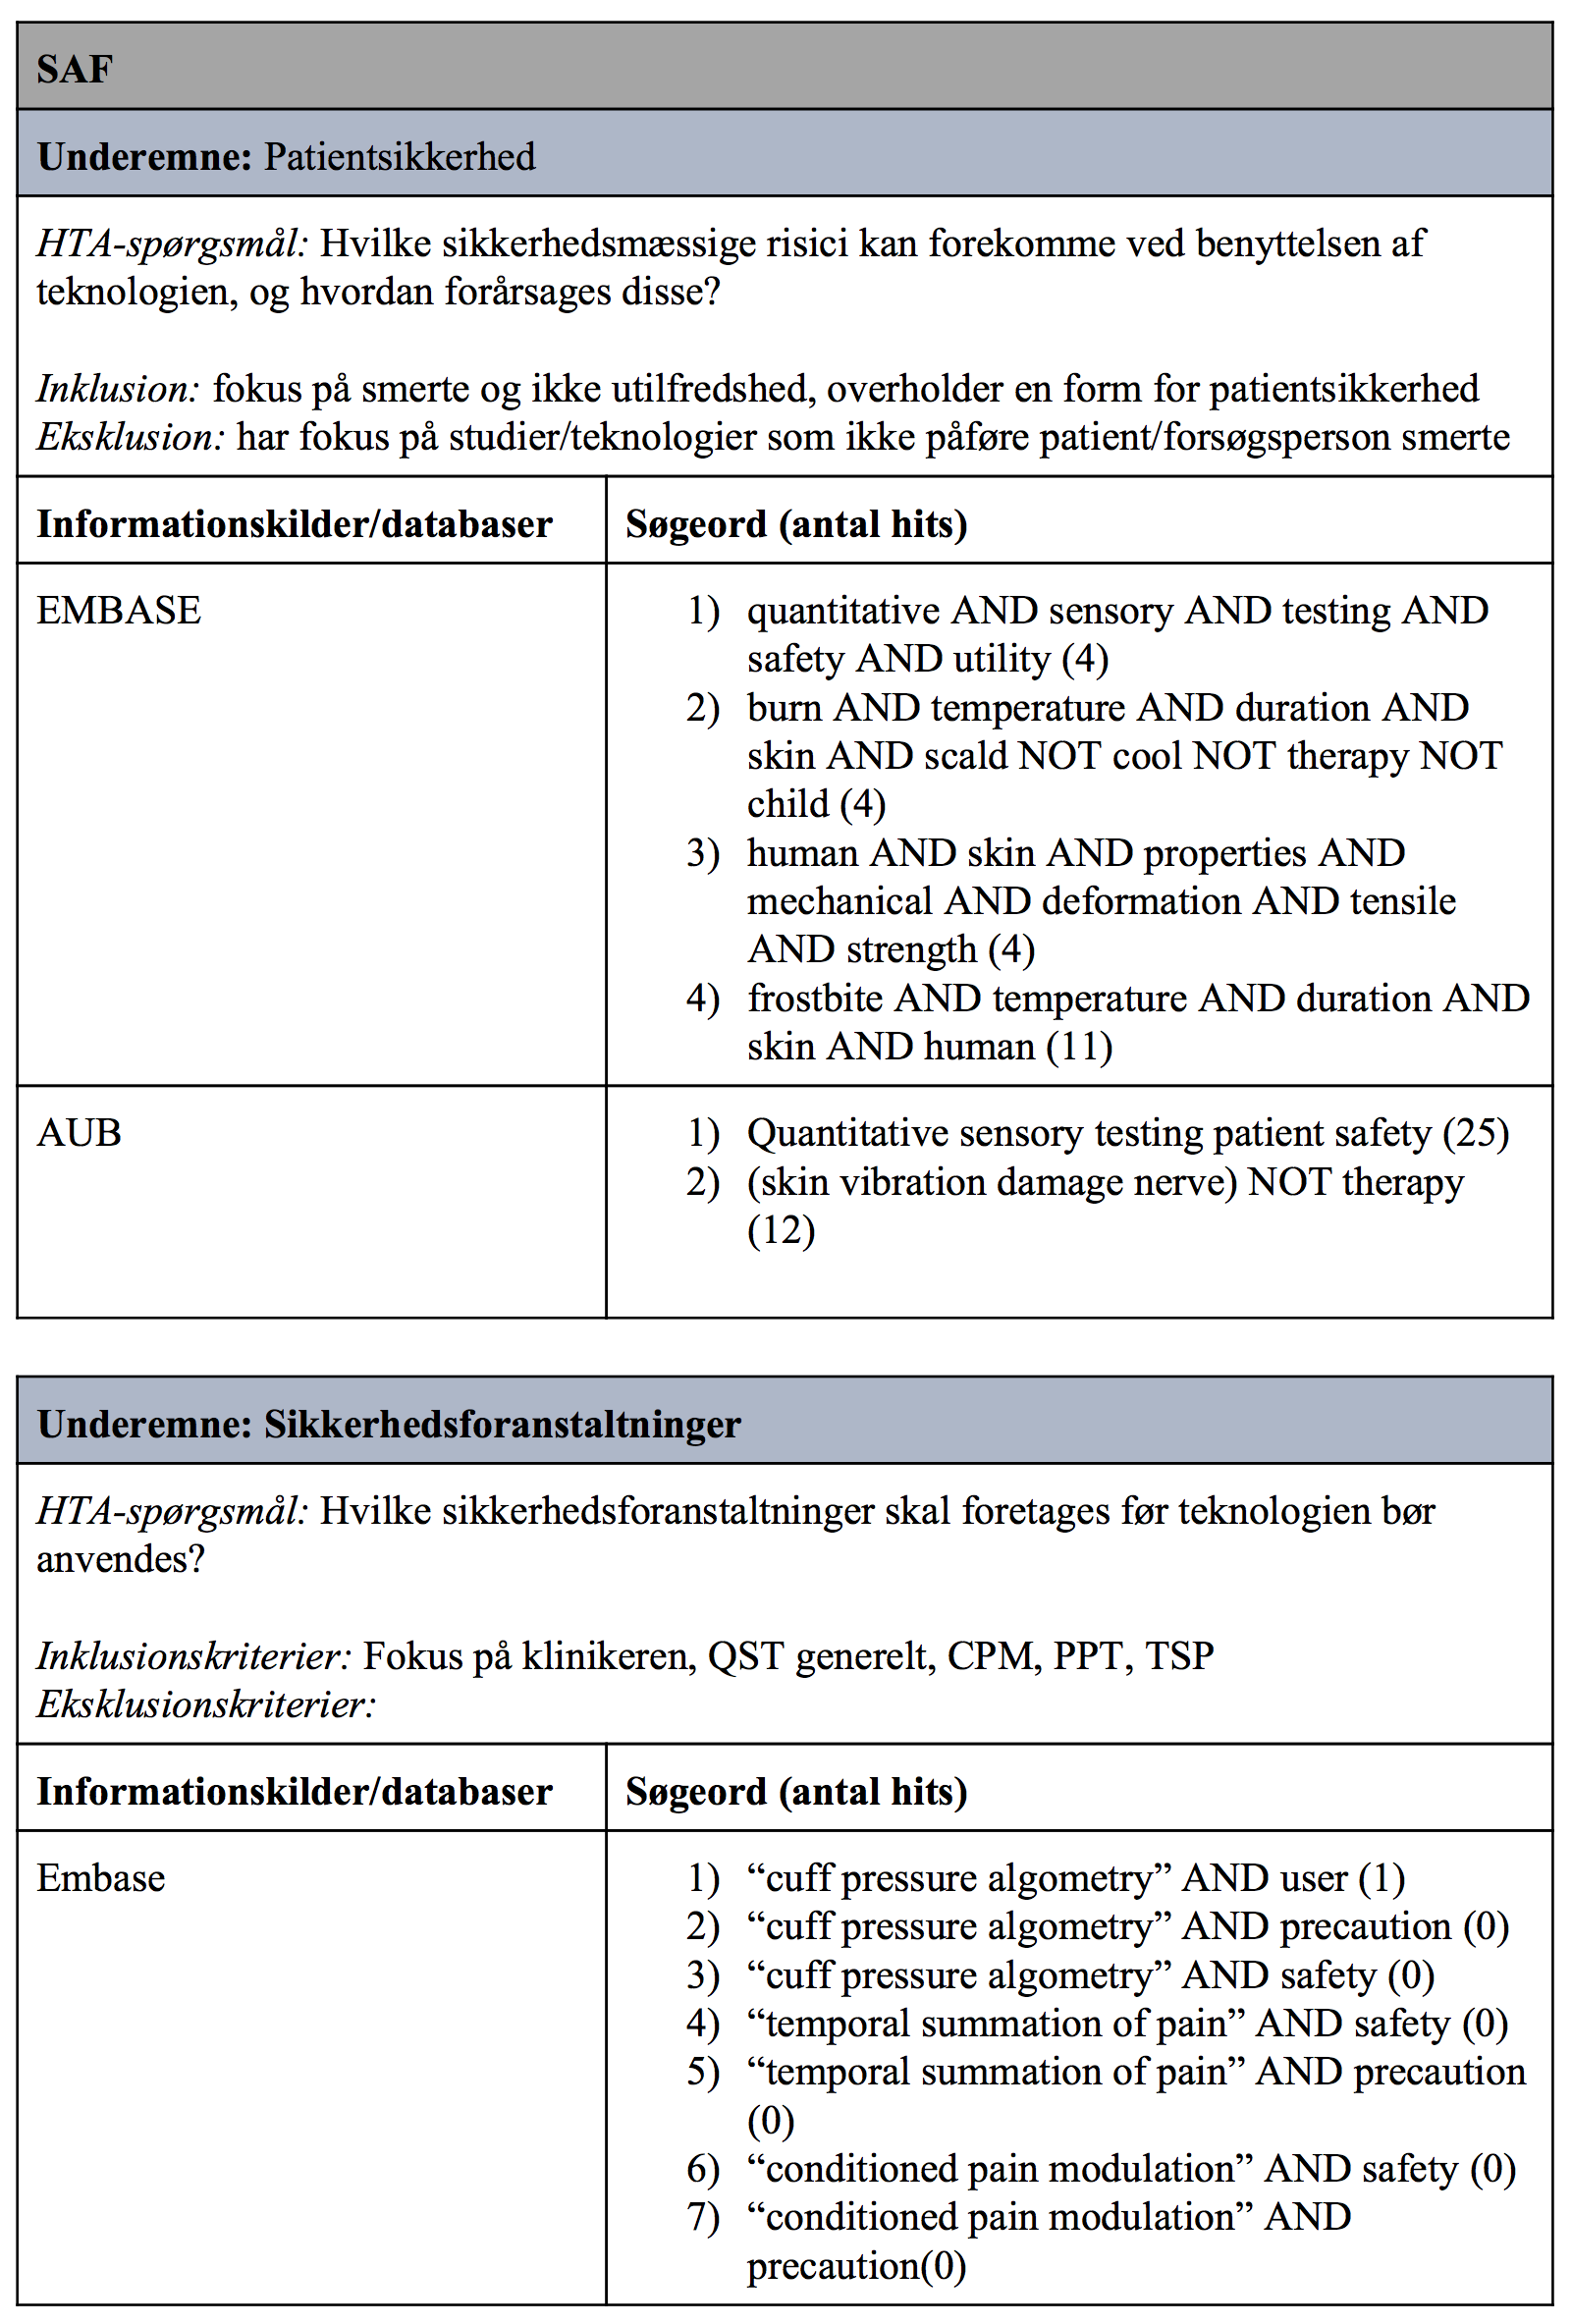
\includegraphics[width=0.8\textwidth]{rapportAfsnit/qBilag/sogninger/SAF1}

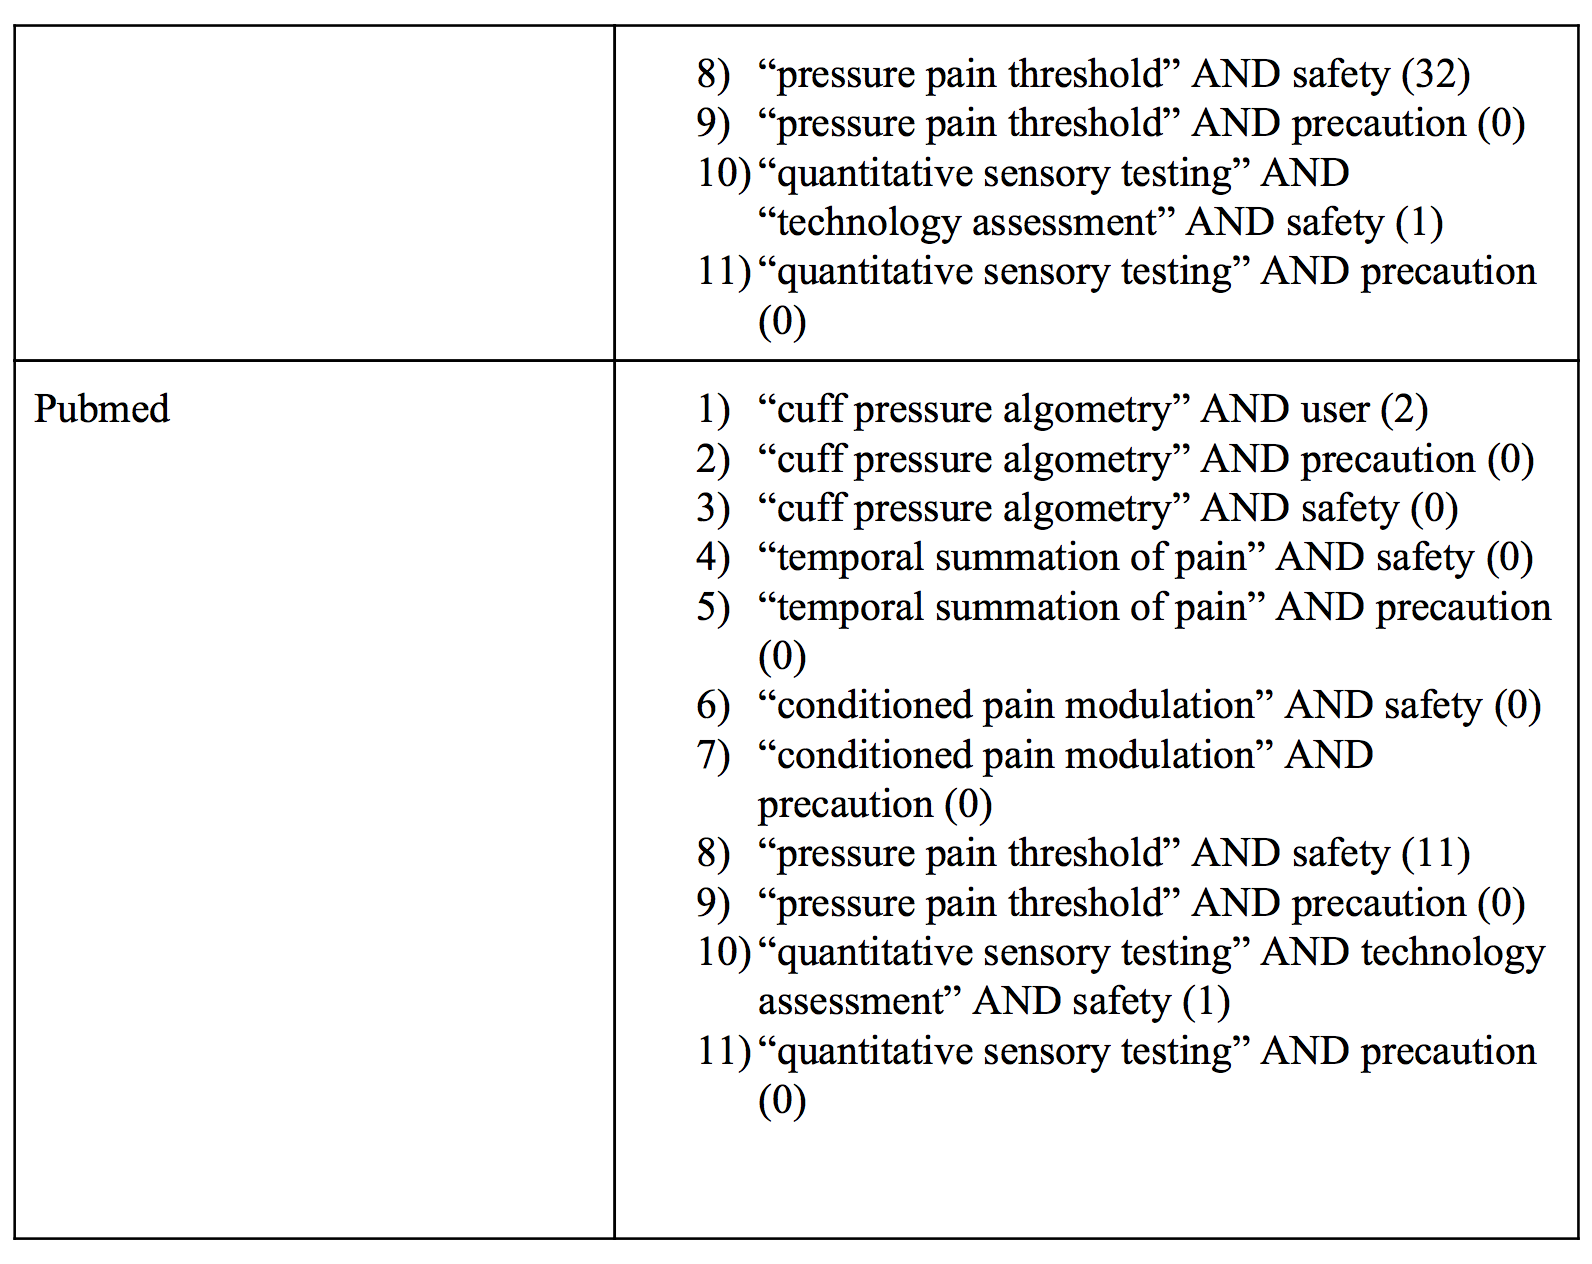
\includegraphics[width=0.8\textwidth]{rapportAfsnit/qBilag/sogninger/SAF2}
\end{center}

\section{SOC}\label{SOC_sog}
\begin{center}
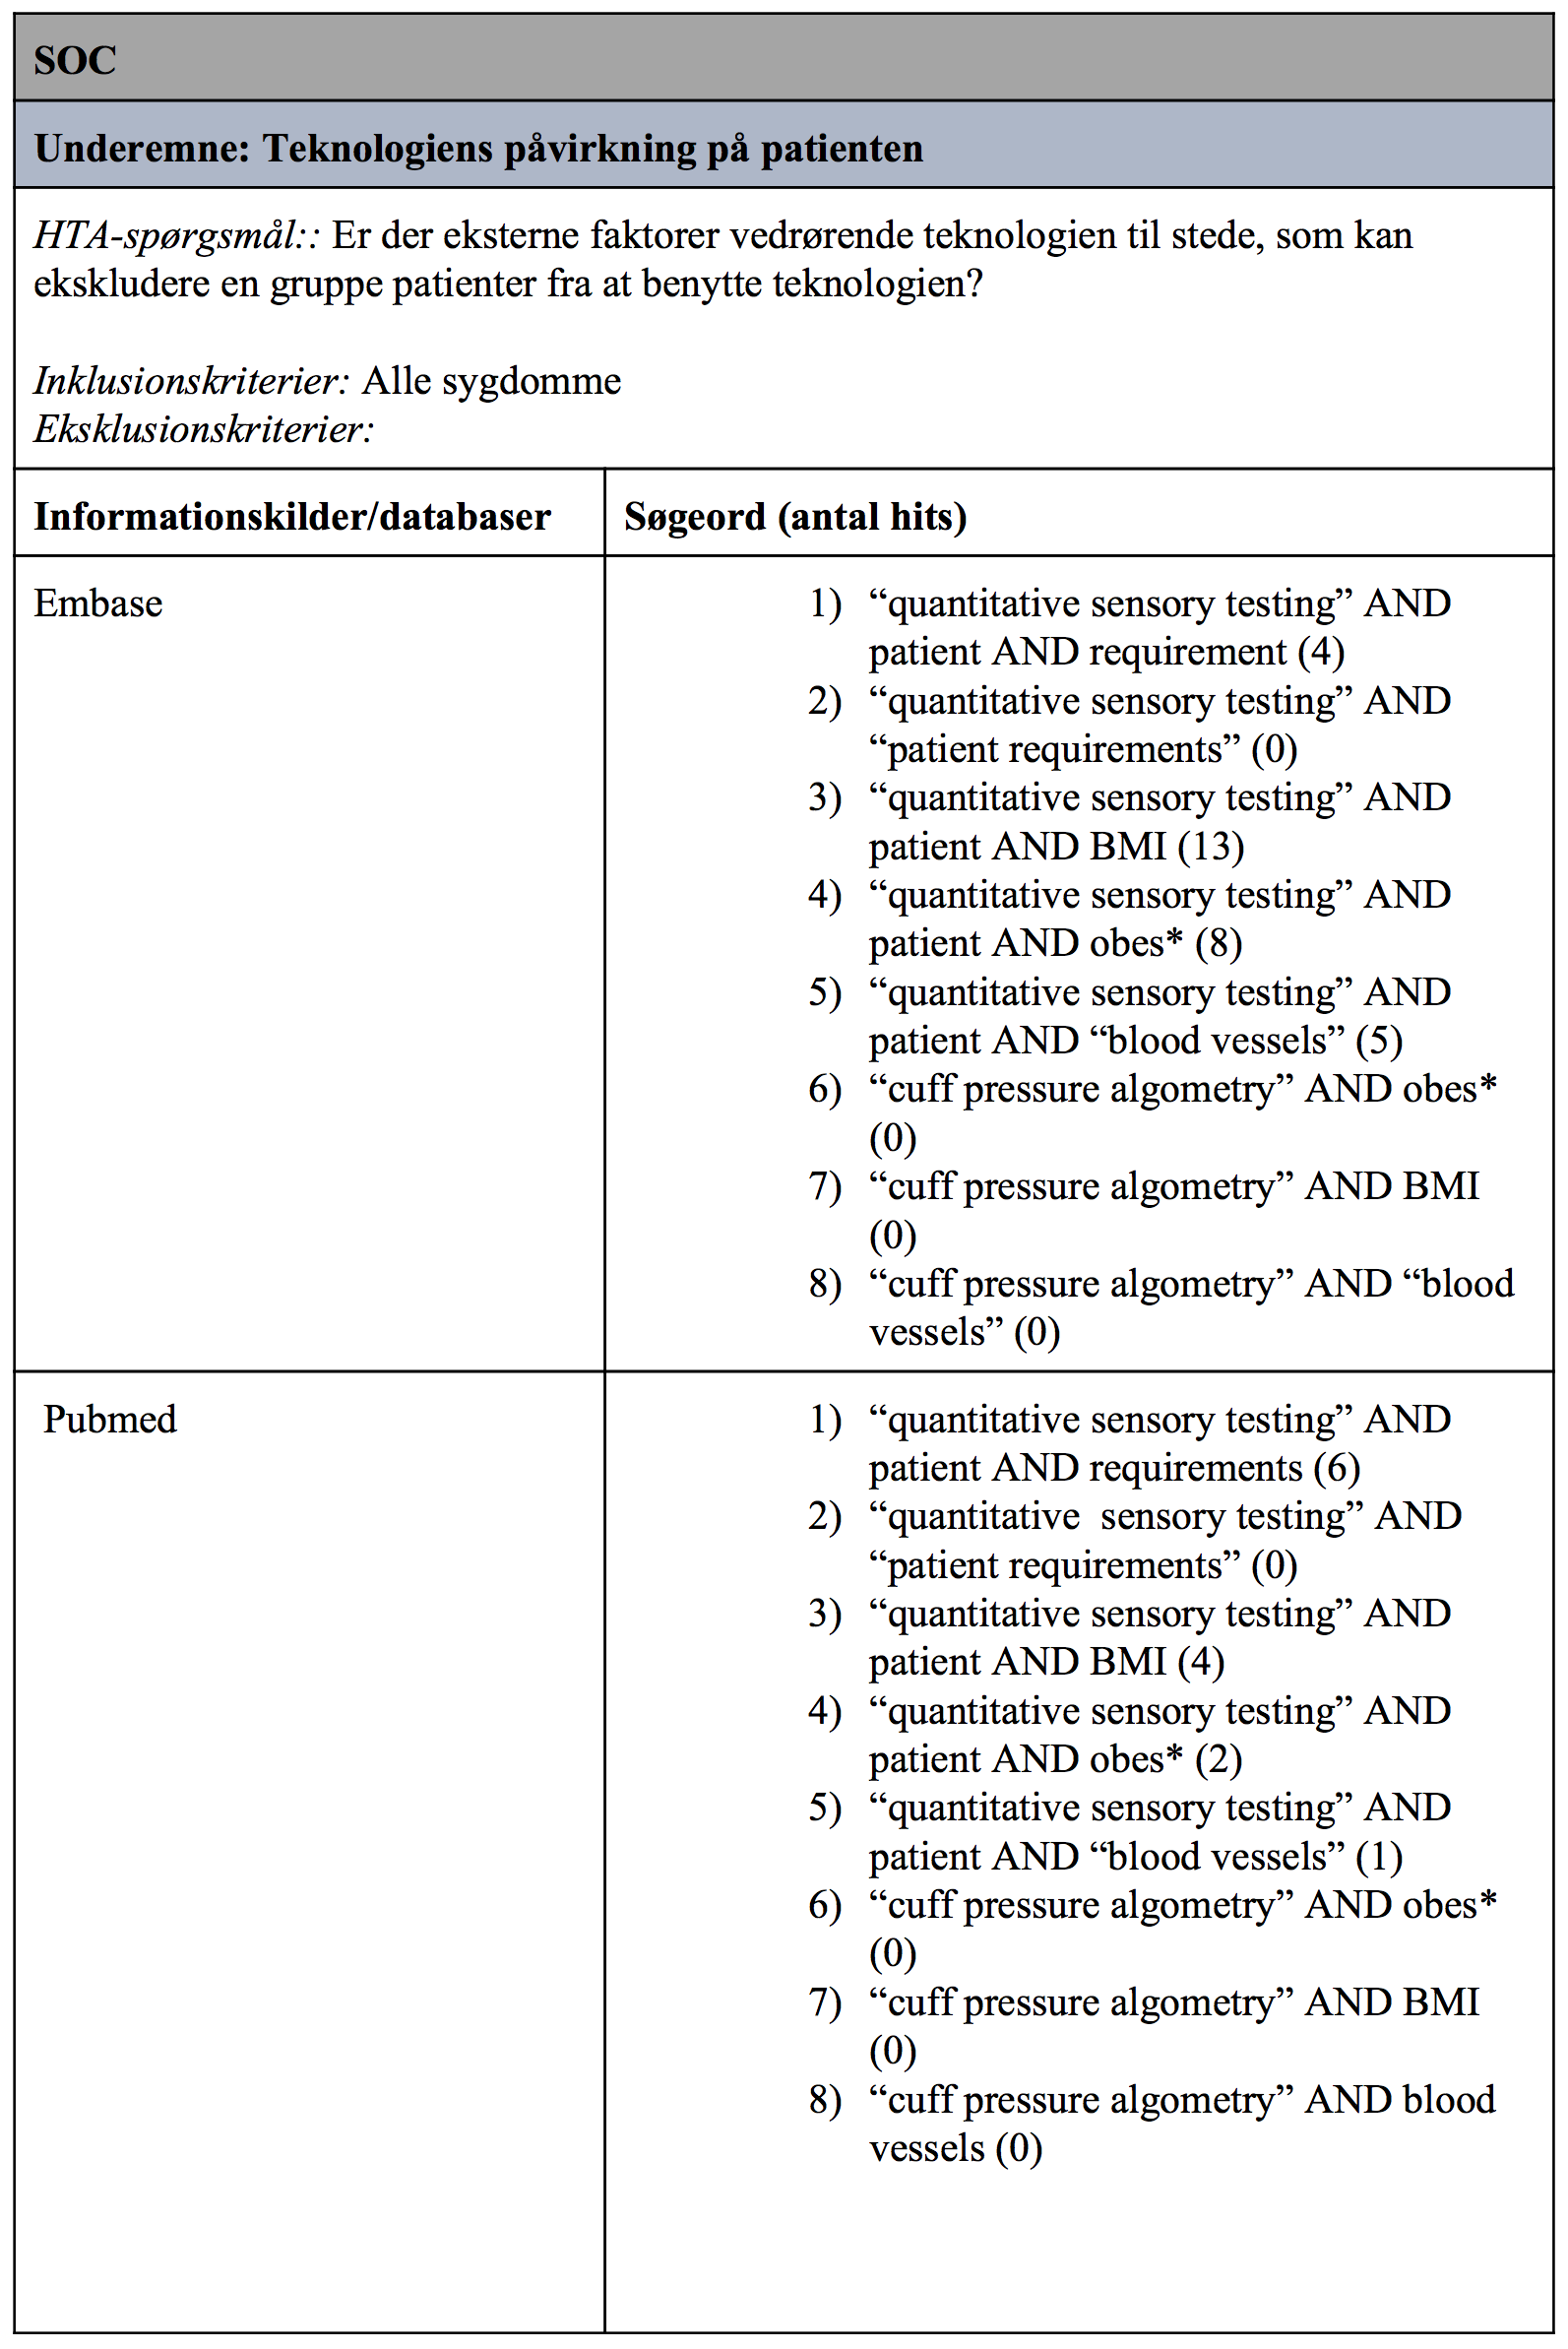
\includegraphics[width=0.8\textwidth]{rapportAfsnit/qBilag/sogninger/SOC1}

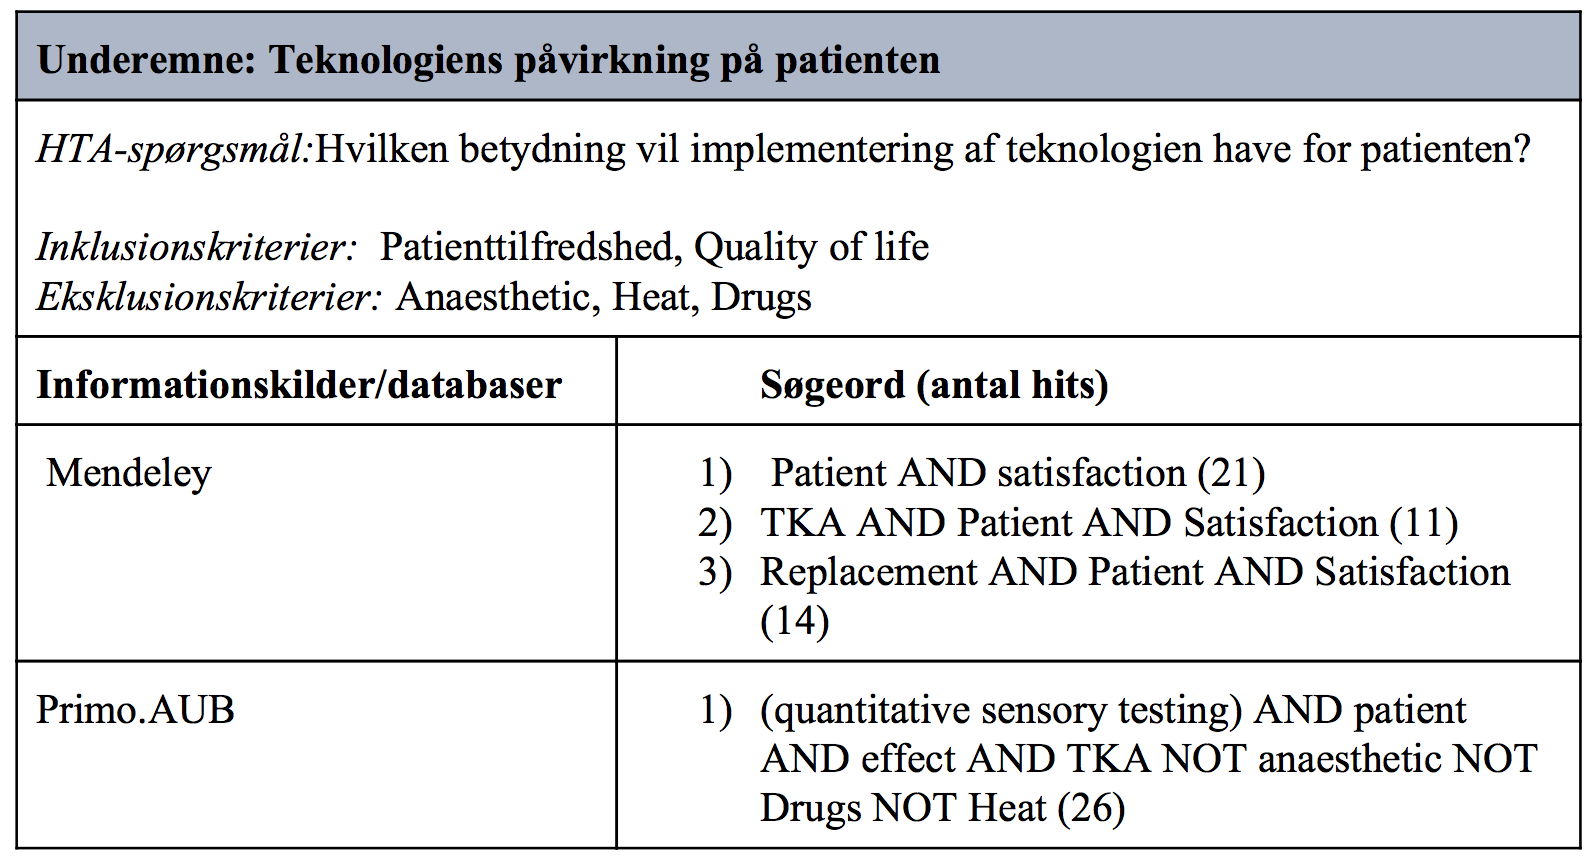
\includegraphics[width=0.8\textwidth]{rapportAfsnit/qBilag/sogninger/SOC2}
\end{center}

\section{ETH}\label{ETH_sog}
\begin{center}
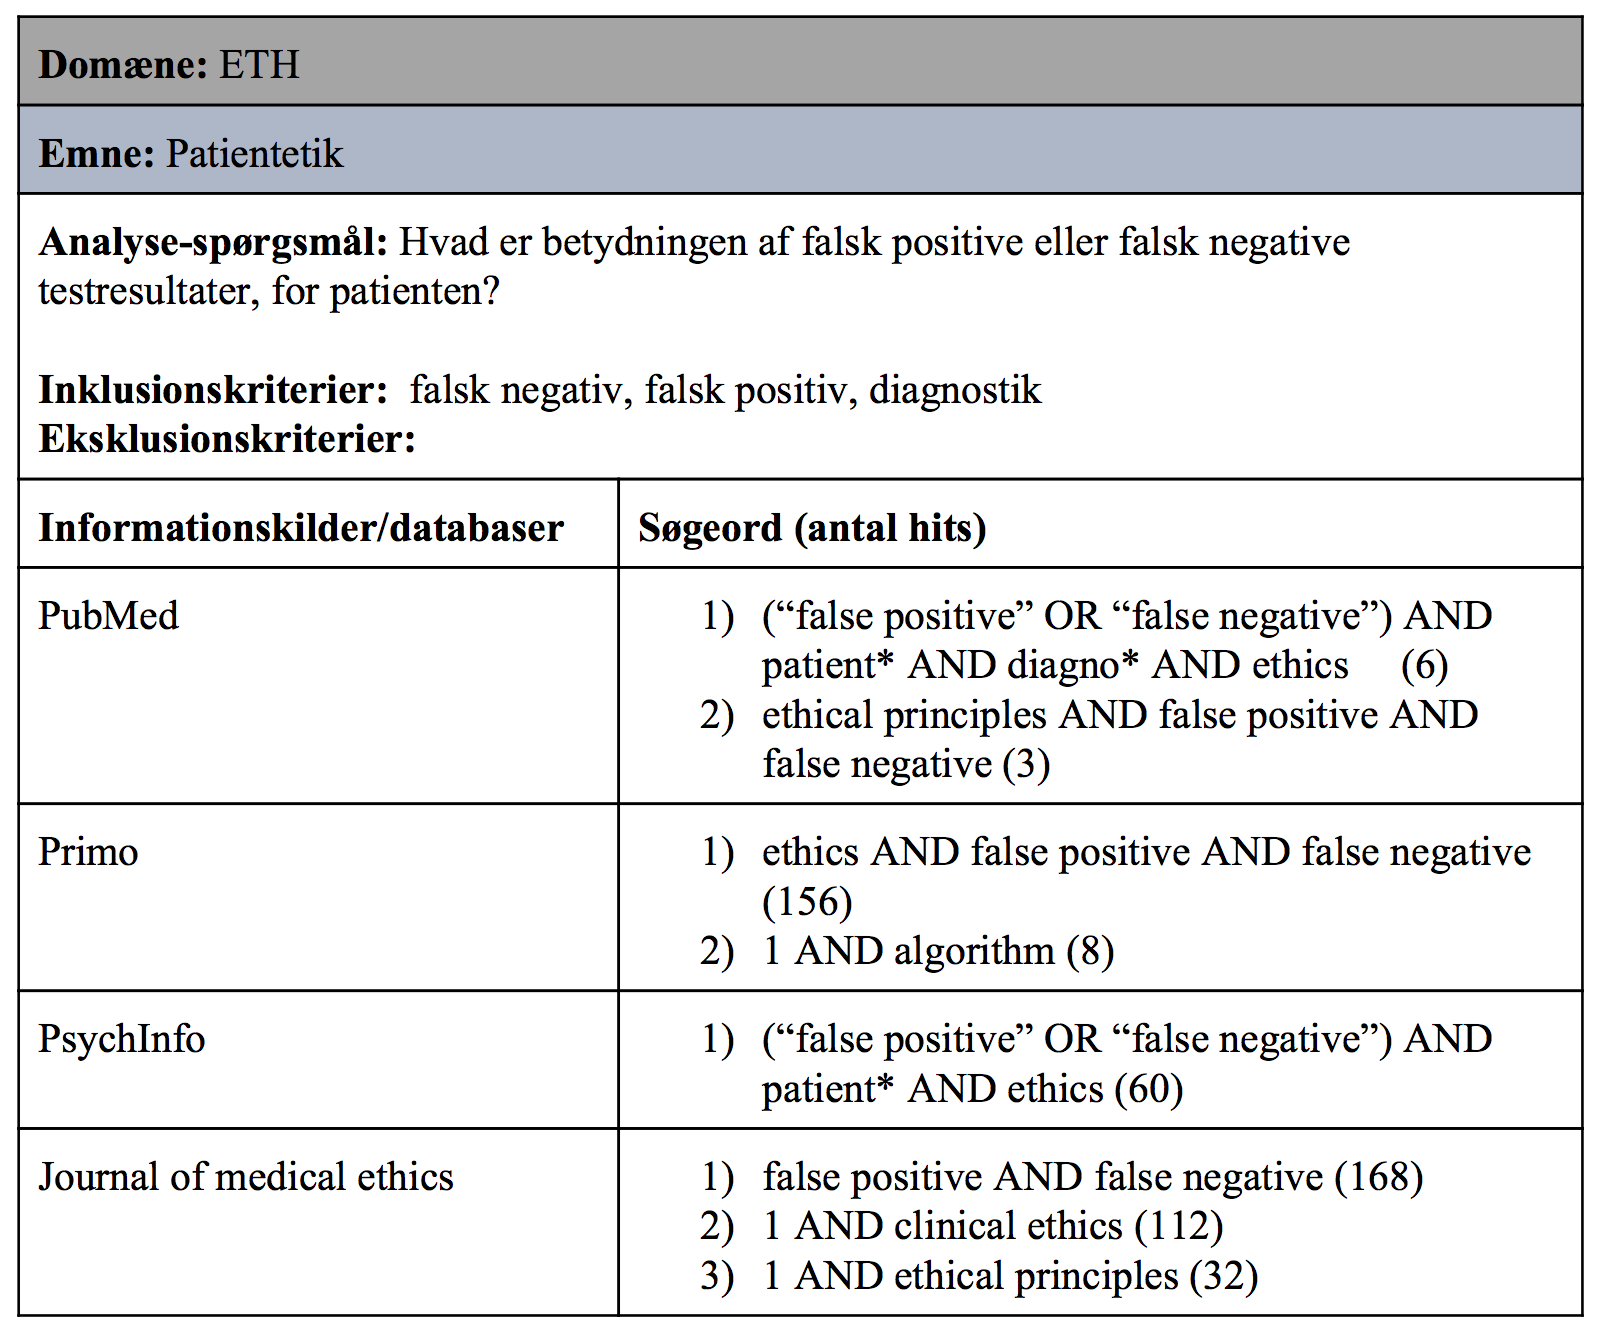
\includegraphics[width=0.8\textwidth]{rapportAfsnit/qBilag/sogninger/ETH1}
\end{center}








%\begin{table}[H]
%\centering
%\caption{My caption}
%\label{my-label}
%\begin{tabular}{|ll|}
%\hline
%\rowcolor[HTML]{656565} 
%{\color[HTML]{000000} \textbf{Problemanalyse}}                                     & {\color[HTML]{656565} }                              \\ \hline
%\textit{Fokuseret sprøgsmål:}                                                      &                                                      \\
%                                                                                   &                                                      \\
%\textit{Inklusion- og ekslusionskriterier:}                                        &                                                      \\
%\textit{Inklusion:}                                                                &                                                      \\
%\textit{Eksklusion:}                                                               &                                                      \\ \hline
%\rowcolor[HTML]{C0C0C0} 
%{\color[HTML]{000000} \textbf{Underemne: Indledning og initierende problem}}       & {\color[HTML]{C0C0C0} }                              \\ \hline
%\textit{Fokuseret spørgsmål:}                                                      &                                                      \\
%                                                                                   &                                                      \\
%\textit{Inklusionskriterier:}                                                      &                                                      \\
%\textit{Eksklusionskriterier:}                                                     &                                                      \\ \hline
%\multicolumn{1}{|l|}{{\color[HTML]{000000} \textbf{Informationskilder/databaser}}} & {\color[HTML]{000000} \textbf{Søgeord (antal hits)}} \\ \hline
%\multicolumn{1}{|l|}{}                                                             &                                                      \\ \hline
%\rowcolor[HTML]{C0C0C0} 
%{\color[HTML]{000000} \textbf{Underemne: Indledning og initierende problem}}       & {\color[HTML]{000000} }                              \\ \hline
%\textit{Fokuseret spørgsmål:}                                                      &                                                      \\
%                                                                                   &                                                      \\
%\textit{Inklusionskriterier:}                                                      &                                                      \\
%\textit{Eksklusionskriterier:}                                                     &                                                      \\ \hline
%\end{tabular}
%\end{table}
\end{appendices}

\end{document}
